\documentclass[sigconf]{acmart}


\usepackage{graphics}
\usepackage{graphicx}
\usepackage{xspace}
\usepackage{subcaption}
\usepackage{amsmath}
\usepackage{amsthm}
%\usepackage{amssymb}
\usepackage{mathrsfs}
\usepackage{array}
\usepackage{textcomp}
\usepackage{weiwAlgorithm}
\usepackage{url}
\usepackage{diagbox}
\usepackage{color}
\usepackage{booktabs}
\usepackage{listings}
\usepackage{tcolorbox}
\usepackage{setspace}
\usepackage{multirow}
\usepackage{booktabs}    % 提供 \toprule, \midrule, \bottomrule
\usepackage{tabularx}    % 提供 tabularx 环境
\usepackage{array}       % 增强表格功能
\usepackage{makecell}    % 便于多行单元格
\usepackage{enumitem}



\sloppy
\textfloatsep 1mm plus 1mm \intextsep 1mm plus 1mm

\usepackage[normalem]{ulem}
\useunder{\uline}{\ul}{}

\newtheorem{example}{Example}
\newtheorem{problem}{Problem}
\newtheorem{remark}{Remark}
\newtheorem{theorem}{Theorem}
\newtheorem{lemma}{Lemma}
\newtheorem{proposition}{Proposition}
\newtheorem{property}{Property}
\newtheorem{conjecture}{Conjecture}
\newtheorem{corollary}{Corollary}
\newtheorem{definition}{Definition}
\newtheorem{descriptioin}{Description}
\newtheorem{extension}{Extension}
\newtheorem{discussion}{Discussion}
\newtheorem{observation}{\textbf{Observation}}

\DeclareMathOperator*{\argmin}{arg\,min}
\DeclareMathOperator*{\argmax}{arg\,max}

\newcommand{\edge}[1]{\left< #1 \right>}
\newcommand{\pr}[1]{\mathcal{P}(#1)}
\newcommand{\wt}[1]{w(#1)}
\newcommand{\Inf}[1]{\sigma(#1)}
\newcommand{\EstInf}[1]{I(#1)}
\newcommand{\bk}{bottom-\emph{k}\xspace}
\newcommand{\skris}{BKRIS\xspace}
\newcommand{\Bk}{Bottom-\emph{k}\xspace}
\newcommand{\ris}{RIS\xspace}

\newcommand{\myparagraph}[1]{\vspace{0.5mm} \noindent \textbf{#1}.}
\newcommand{\myparagraphnew}[1]{\noindent \textbf{#1}.}
\newcommand{\myparagraphunderline}[1]{\vspace{0.5mm} \noindent \underline{#1.}}
\newcommand{\myparagraphquestion}[1]{\vspace{0.5mm} \noindent \textbf{#1?}}
\newcommand{\myparagraphunderlinenew}[1]{\vspace{0.5mm} \noindent \underline{#1,}}

\newcommand{\ie}{{i.e.,}\xspace}
\newcommand{\eg}{{e.g.,}\xspace}
\newcommand{\etal}{et al.\xspace}
\newcommand{\set}[1]{\{#1\}}



%% \BibTeX command to typeset BibTeX logo in the docs
% \AtBeginDocument{%
%   \providecommand\BibTeX{{%
%     \normalfont B\kern-0.5em{\scshape i\kern-0.25em b}\kern-0.8em\TeX}}}

\long\def\appendixsiam{\par\setcounter{section}{0}\setcounter{subsection}{0}\setcounter{equation}{0}}
\AtBeginDocument{%
  \providecommand\BibTeX{{%
    Bib\TeX}}}



\copyrightyear{2025}
\acmYear{2025}
\setcopyright{acmlicensed}\acmConference[WWW '25]{Proceedings of the ACM Web Conference 2025}{April 28-May 2, 2025}{Sydney, NSW, Australia}
\acmBooktitle{Proceedings of the ACM Web Conference 2025 (WWW '25), April 28-May 2, 2025, Sydney, NSW, Australia}
\acmDOI{10.1145/3696410.3714892}
\acmISBN{979-8-4007-1274-6/25/04}

\begin{document}
\lstdefinelanguage{SPARQL}{
  morekeywords={BASE,PREFIX,SELECT,WHERE,FILTER,OPTIONAL,DISTINCT,GRAPH,UNION,ASK,CONSTRUCT,DESCRIBE,FROM,NAMED,ORDER,BY,ASC,DESC,LIMIT,OFFSET,BIND,VALUES},
  sensitive=false,
  morecomment=[l]{\#},
  morestring=[b]",
}
  % 增强表格功能

\lstset{
  language=SPARQL,
  basicstyle=\ttfamily\small,
  commentstyle=\color{green},
  keywordstyle=\color{blue},
  stringstyle=\color{red},
  breaklines=true,
  escapechar=|, % 定义转义字符为|
}

% \title{Map-In-Graph: Deep and Responsible Meta Entities Reasoning of Large Language Model on Knowledge Graph}
% \title{Walking-In-Graph: Deep and Responsible Complex Question Reasoning Large Language Model on Knowledge Graph}

\title{Paths-over-Graph: Knowledge Graph Empowered Large Language Model Reasoning}


% \title{Paths-In-Graph: LLM Empowered Path-based Faithful and  Reliable Reasoning on Knowledge Graph}

\author{Xingyu Tan}
\orcid{0009-0000-7232-7051}
\affiliation{%
  \institution{University of New South Wales}
  \institution{Data61, CSIRO}
  \city{Sydney}
  \country{Australia}}
\email{xingyu.tan@unsw.edu.au}

\author{Xiaoyang Wang}
\orcid{0000-0003-3554-3219}
\affiliation{%
  \institution{University of New South Wales}
  \city{Sydney}
  \country{Australia}}
\email{xiaoyang.wang1@unsw.edu.au}
\authornote{Corresponding author.}

\author{Qing Liu}
\orcid{0000-0001-7895-9551}
\affiliation{%
  \institution{Data61, CSIRO}
  \city{Sydney}
  \country{Australia}}
\email{q.liu@data61.csiro.au}

\author{Xiwei Xu}
\orcid{0000-0002-2273-1862}
\affiliation{%
  \institution{Data61, CSIRO}
  \city{Sydney}
  \country{Australia}}
\email{xiwei.xu@data61.csiro.au}

\author{Xin Yuan}
\orcid{0000-0002-9167-1613}
\affiliation{%
  \institution{Data61, CSIRO}
  \city{Sydney}
  \country{Australia}}
\email{xin.yuan@data61.csiro.au}


\author{Wenjie Zhang}
\orcid{0000-0001-6572-2600}
\affiliation{%
  \institution{University of New South Wales}
  \city{Sydney}
  \country{Australia}}
\email{wenjie.zhang@unsw.edu.au}

\renewcommand{\shortauthors}{Xingyu Tan et al.}





% \renewcommand{\shortauthors}{a}


\begin{abstract}

Large Language Models (LLMs) have achieved impressive results in various tasks but struggle with hallucination problems and lack of relevant knowledge, especially in deep complex reasoning and knowledge-intensive tasks. Knowledge Graphs (KGs), which capture vast amounts of facts in a structured format, offer a reliable source of knowledge for reasoning. However, existing KG-based LLM reasoning methods face challenges like handling multi-hop reasoning, multi-entity questions, and effectively utilizing graph structures. To address these issues, we propose Paths-over-Graph (PoG), a novel method that enhances LLM reasoning by integrating knowledge reasoning paths from KGs, improving the interpretability and faithfulness of LLM outputs. PoG tackles multi-hop and multi-entity questions through a three-phase dynamic multi-hop path exploration, which combines the inherent knowledge of LLMs with factual knowledge from KGs. In order to improve the efficiency, PoG prunes irrelevant information from the graph exploration first and introduces efficient three-step pruning techniques that incorporate graph structures, LLM prompting, and a pre-trained language model (e.g., SBERT) to effectively narrow down the explored candidate paths.  This ensures all reasoning paths contain highly relevant information captured from KGs, making the reasoning faithful and interpretable in problem-solving. PoG innovatively utilizes graph structure to prune the irrelevant noise and represents the first method to implement multi-entity deep path detection on KGs for LLM reasoning tasks. Comprehensive experiments on five benchmark KGQA datasets demonstrate PoG outperforms the state-of-the-art method ToG across GPT-3.5-Turbo and GPT-4, achieving an average accuracy improvement of 18.9\%. Notably, PoG with GPT-3.5-Turbo surpasses ToG with GPT-4 by up to 23.9\%. 

\end{abstract}

% \begin{CCSXML}
% <ccs2012>
%    <concept>
%        <concept_id>10002951.10002952.10002953.10010146.10010818</concept_id>
%        <concept_desc>Information systems~Network data models</concept_desc>
%        <concept_significance>500</concept_significance>
%        </concept>
%  </ccs2012>
% \end{CCSXML}

% \ccsdesc[500]{Information systems~Network data models}
\vspace{-4mm}
\begin{CCSXML}
<ccs2012>
   <concept>
       <concept_id>10002951.10003317.10003347.10003348</concept_id>
       <concept_desc>Information systems~Question answering</concept_desc>
       <concept_significance>500</concept_significance>
       </concept>
 </ccs2012>
\end{CCSXML}
\ccsdesc[500]{Information systems~Question answering}
% %%
% %% Keywords. The author(s) should pick words that accurately describe
% %% the work being presented. Separate the keywords with commas.
\keywords{Large Language Models; Knowledge Graph;  Knowledge Graph Question Answering; Retrieval-Augmented Generation}


\maketitle



% \vspace{-2mm}
\section{Introduction}
\label{sec:1_intro}
\captionsetup[table]{aboveskip=6pt, belowskip=6pt} % 标题与表格上/下方距离
\begin{figure}[t]
    \centering
    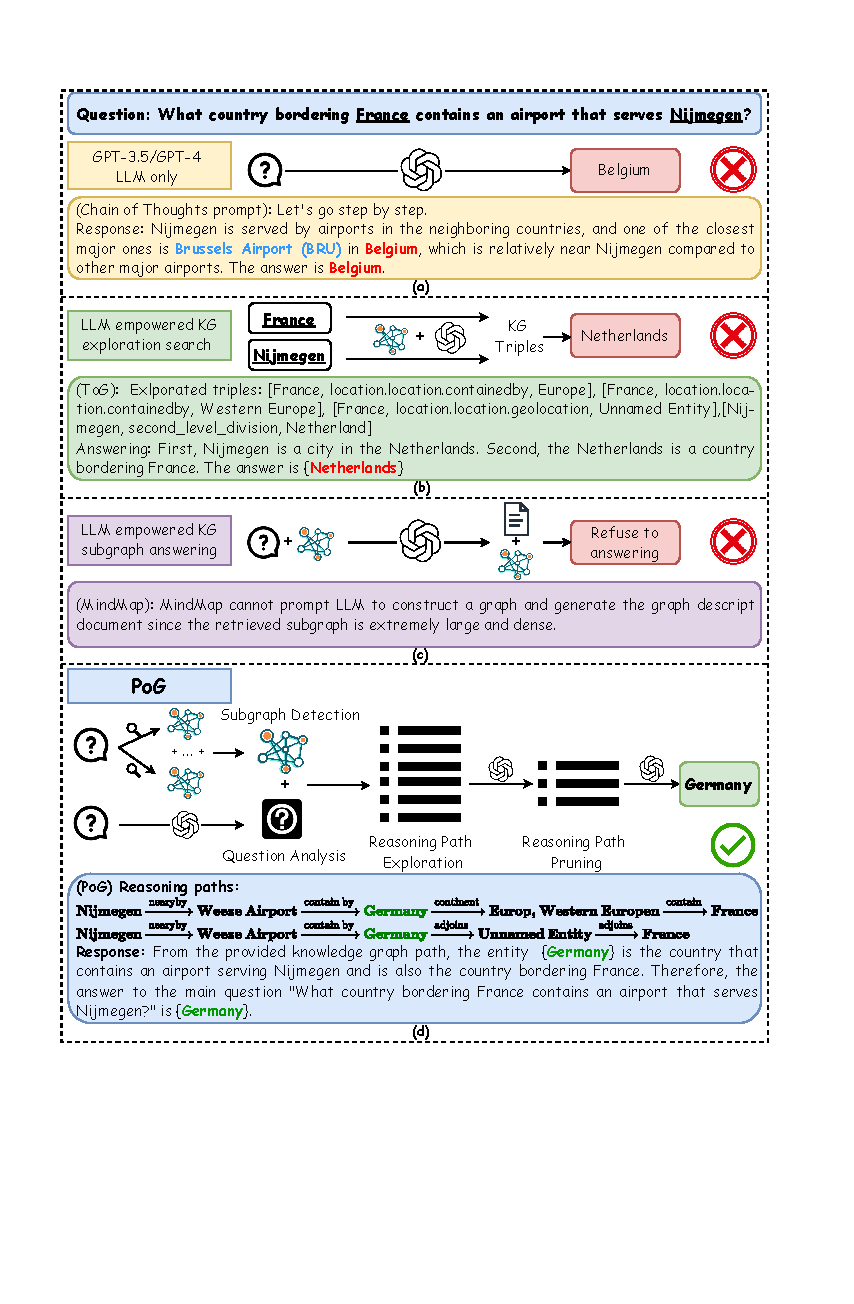
\includegraphics[width=0.9\linewidth]{graphs/baslineworkflow.pdf}
    \vspace{-5pt}
    \caption{Representative workflow of four LLM reasoning paradigms.}
    \label{fig:intro_demo}
\end{figure}


Large Language Models (LLMs) have demonstrated remarkable performance in various tasks \cite{brown2020language,chowdhery2023palm,touvron2023llama,besta2024graphGoT,huang-etal-2025-embedding}. These models leverage pre-training techniques by scaling to billions of parameters and training on extensive, diverse, and unlabelled data \cite{touvron2023llama,rawte2023survey}.
% Firstly it is difficult to process deep and responsible reasoning when solving complex tasks\cite{petroni2020kilt, talmor2018commonsenseqa,khot2022decomposed}. 
Despite these impressive capabilities, LLMs face two well-known challenges. 
First, they struggle with deep and responsible reasoning when tackling complex tasks \cite{petroni2020kilt, talmor2018commonsenseqa,khot2022decomposed}.
Second, the substantial cost of training makes it difficult to keep models updated with the latest knowledge \cite{tog1.0sun2023think,mindmapwen2023}, leading to errors when answering questions that require specialized
information not included in their training data. 
% For example in the Figure~\ref{fig:intro_demo}.1, with the knowledge-specific question, GPT can attempt a reasonable answering strategy 
For example, in Figure~\ref{fig:intro_demo}(a), though models like GPT can generate reasonable answers for knowledge-specific questions, 
these answers may be incorrect due to outdated information or hallucination of reasoning on LLM inherent Knowledge Base (KB).



To deal with the problems of error reasoning and knowledge gaps, the \texttt{plan-retrieval-answering} method has been proposed \cite{rogluo2023reasoning,zhao2023verify,li2023chaincok}. In this approach, LLMs are prompted to decompose complex reasoning tasks into a series of sub-tasks, forming a \texttt{plan}. Simultaneously, external KBs are retrieved to answer each step of the plan. 
However, this method still has the issue of heavily relying on the reasoning abilities of LLMs rather than the faithfulness of the retrieved knowledge. The generated reasoning steps guide information selection, but answers are chosen based on the LLM's interpretation of the retrieved knowledge rather than on whether the selection leads to a correct and faithful answer.

To address these challenges, incorporating external knowledge sources like Knowledge Graphs (KGs) is a promising solution to enhance LLM reasoning~\cite{tog1.0sun2023think, rogluo2023reasoning, pan2024unifying, luo2023chatrule}. KGs offer abundant factual knowledge in a structured format, serving as a reliable source to improve LLM capabilities.  
Knowledge Graph Question Answering (KGQA) serves as an approach for evaluating the integration of KGs with LLMs,
which requires machines to answer natural language questions by retrieving relevant facts from KGs.
These approaches typically involve: (1) identifying the initial entities from the question, and (2) iteratively retrieving and refining inference paths until sufficient evidence has been obtained. 
Despite their success, they still face challenges such as handling multi-hop reasoning problems, addressing questions with multiple topic entities, and effectively utilizing the structural information of graphs.



\myparagraphunderline{Challenge 1: Multi-hop reasoning problem} Current methods \cite{guo2024knowledgenavigator,ye2021rng,tog1.0sun2023think,tog2.0ma2024think}, such as the ToG model presented in Figure~\ref{fig:intro_demo}(b), begin by exploring from each topic entity, with LLMs selecting connected knowledge triples like \texttt{(France, contained\_by, Europe)}. This process relies on the LLM's inherent understanding of these triples. However, focusing on one-hop neighbors can result in plausible but incorrect answers and prematurely exclude correct ones, especially when multi-hop reasoning is required. 
Additionally, multi-hop reasoning introduces significant computational overhead, making efficient pruning essential, especially in dense and large KGs.







\myparagraphunderline{Challenge 2: Multi-entity question} As shown in Figure \ref{fig:intro_demo}(b), existing work \cite{guo2024knowledgenavigator,ye2021rng,tog1.0sun2023think,tog2.0ma2024think} typically explores KG for each topic entity independently. When a question involves multiple entities, these entities are examined in separate steps without considering their interconnections. This approach can result in a large amount of irrelevant information in the candidate set that does not connect to the other entities in the question, leading to suboptimal results. 

\myparagraphunderline{Challenge 3: Utilizing graph structure} 
Existing methods~\cite{mindmapwen2023, guo2023gpt4graph, chen2024exploring} often overlook the inherent graph structures when processing retrieved subgraphs.
For example, the MindMap model in Figure \ref{fig:intro_demo}(c) utilizes LLMs to generate text-formatted subgraphs from KG triples, converting them into graph descriptions that are fed back into the LLM to produce answers. This textual approach overlooks the inherent structural information of graphs and can overwhelm the LLM when dealing with large graphs. Additionally, during KG information selection, most methods use in-context learning by feeding triples into the LLM, ignoring the overall graph structure.


\myparagraph{Contributions} In this paper, we introduce a novel method, \textbf{P}aths-\textbf{o}ver-\textbf{G}raph (\textbf{PoG}). Unlike previous studies that utilize knowledge triples for retrieval \cite{tog1.0sun2023think,tog2.0ma2024think}, PoG employs knowledge reasoning paths,
that contain all the topic entities in a long reasoning length,
as a retrieval-augmented input for LLMs. The paths in KGs serve as logical reasoning chains, providing KG-supported, interpretable reasoning logic that addresses issues related to the lack of specific knowledge background and unfaithful reasoning paths.

\myparagraphunderlinenew{To address multi-hop reasoning problem} as shown in Figure \ref{fig:intro_demo}(d), PoG first performs question analysis, to extract topic entities from questions. Utilizing these topic entities, it decomposes the complex question into sub-questions and generates an LLM thinking indicator termed \texttt{"Planning"}.
This planning not only serves as an answering
strategy but also predicts the implied relationship depths between the answer and each topic entity. 
% The multi-hop paths are then explored from the predicted depth up to a user-defined maximum depth.
The multi-hop paths are then explored starting from a predicted depth, enabling a dynamic search process. 
Previous approaches using \texttt{planning} usually retrieve information from scratch, which often confuses LLMs with source neighborhood-based semantic information. In contrast, our method ensures that LLMs follow accurate reasoning paths that directly lead to the answer.
% 


\myparagraphunderlinenew{To address multi-entity questions}
% PoG employs a three-phase exploration process to traverse the reasoning paths from the retrieved question subgraph. All paths must contain all the topic entities in the same order as they appear in the LLM thinking indicator. 
PoG employs a three-phase exploration process to traverse reasoning paths from the retrieved question subgraph. All paths must contain all topic entities in the same order as they occur in the LLM thinking indicator. 
In terms of reasoning paths in KGs, all paths are inherently logical and faithful. Each path potentially contains one possible answer and serves as the interpretable reasoning logic.  The exploration leverages the inherent knowledge of both  LLM and KG.

% Each path in KGs is inherently logical and faithful, potentially containing one possible answer and serving as interpretable answering logic. The exploration leverages the inherent knowledge of the LLM and KG.
\myparagraphunderlinenew{To effectively utilize graph structure} 
PoG captures the question subgraph by expanding topic entities to their maximal depth neighbors, applying graph clustering and reduction to reduce graph search costs.
In the path pruning phase, we select possible correct answers from numerous candidates. All explored paths undergo a three-step beam search pruning, integrating graph structures, LLM prompting, and a pre-trained language understanding model (e.g., BERT) to ensure effectiveness and efficiency. 
Additionally, inspired by the Graph of Thought (GoT) \cite{besta2024graphGoT}, to reduce LLM hallucination, PoG prompts LLMs to summarize the obtained Top-$W_{\max}$ paths before evaluating the answer, where $W_{\max}$ is a user-defined maximum width in the path pruning phase.
In summary, 
the advantage of PoG can be abbreviated as: 
\begin{itemize}[leftmargin=*]
\item \textbf{Dynamic deep search}: Guided by LLMs, PoG dynamically extracts multi-hop reasoning paths from KGs, enhancing LLM capabilities in complex knowledge-intensive tasks.
\item \textbf{Interpretable and faithful reasoning}: 
By utilizing highly question-relevant knowledge paths, PoG improves the interpretability of LLM reasoning, enhancing the faithfulness and question-relatedness of LLM-generated content.
\item \textbf{Efficient pruning with graph structure integration}: 
% To reduce computational costs and mitigate LLM hallucinations caused by irrelevant noise, PoG incorporates efficient pruning techniques in both the knowledge graph and reasoning paths. 
% Pruning irrelevant data through graph reduction significantly reduces computational overhead. The path pruning process integrates non-LLM methods, LLM prompting, and graph structural analysis to effectively narrow down the candidate set.
PoG incorporates efficient pruning techniques in both the KG and reasoning paths to reduce computational costs, mitigate LLM hallucinations caused by irrelevant noise, and effectively narrow down candidate answers.
\item \textbf{Flexibility and effectiveness}:
a) PoG is a plug-and-play framework that can be seamlessly applied to various LLMs and KGs.
b) PoG allows frequent knowledge updates via the KG, avoiding the expensive and slow updates required for LLMs.
c) PoG reduces the LLMs token usage by over 50\% with only a ±2\% difference in accuracy compared to the best-performing strategy.
d) PoG achieves state-of-the-art results on all the tested KGQA datasets, outperforming the strong baseline ToG by an average of 18.9\% accuracy using both GPT-3.5 and GPT-4. Notably, PoG with GPT-3.5 can outperform ToG with GPT-4 by up to 23.9\%.
\end{itemize}
\vspace{-3mm}



\section{Related Work}\label{sec:related_work}
\noindent \textbf{KG-based LLM reasoning}.
KGs provide structured knowledge valuable for integration with LLMs~\cite{pan2024unifying}. Early studies~\cite{peters2019knowledge, rogluo2023reasoning, zhang2021poolingformer, li2023chaincok} embed KG knowledge into neural networks during pre-training or fine-tuning, but this can reduce explainability and hinder efficient knowledge updating~\cite{pan2024unifying}.
Recent methods combine KGs with LLMs by converting relevant knowledge into textual prompts, often ignoring structural information~\cite{pan2024unifying, mindmapwen2023}. Advanced works~\cite{tog1.0sun2023think, jiang2023structgpt, tog2.0ma2024think} involve LLMs directly exploring KGs, starting from an initial entity and iteratively retrieving and refining reasoning paths until the LLM decides the augmented knowledge is sufficient.
However, by starting from a single vertex and ignoring the question's position within the KG's structure, these methods overlook multiple topic entities and the explainability provided by multi-entity paths. 
 
% However, these methods often ignore the question's position within the KG's graph structure, starting exploration from a single vertex. This approach overlook the importance of multiple topic entities and the explainability provided by multi-entity paths. fail in long reasoning tasks because the LLM considers only local semantic contexts rather than a global perspective. 
% Moreover, when questions involve multiple entities, they overlook the importance of multiple topic entities and the explainability provided by multi-entity paths. They also typically impose a uniform depth limit, which may not be optimal for all queries.




% \myparagraph{KG-Based LLM Reasoning}KGs offer dynamic, explicit, and structured knowledge representations, making them valuable for integration with LLMs\cite{pan2024unifying}. Early studies \cite{peters2019knowledge, rogluo2023reasoning,zhang2021poolingformer,li2023chaincok} focused on embedding structured knowledge from KGs into neural networks during pre-training or fine-tuning. However, embedding KGs within LLMs can sacrifice explainability in knowledge reasoning and hinder efficient knowledge updating\cite{pan2024unifying}.
% Recent works combine KGs with LLMs by translating relevant structured knowledge into textual prompts, often involving converting the graph into natural language input for the LLM, which ignores the inherent structural information\cite{pan2024unifying,tog1.0sun2023think}. Alternatively, more advanced works \cite{tog1.0sun2023think, jiang2023structgpt,tog2.0ma2024think} involve LLMs in exploring KGs directly, usually identify the initial entity in the question, then to iteratively retrieve and refine the reasoning path until LLM to decide the augmented knowledge is sufficient.
% These existing methods, while effective to some extent, tend to ignore the positional information of the question within the KG's graph structure. They often start exploration from a single vertex, using KG triples as knowledge fed into the LLM to form new reasoning paths. This approach can fail during long reasoning tasks because the LLM considers only local semantic contexts rather than a global perspective. Moreover, when questions involve multiple entities, existing methods overlook the importance of multiple topic entities and the explainability provided by multi-entity paths in question answering. They also typically impose a broad, uniform depth limit for reasoning deep questions, which may not be optimal for all queries.

\myparagraph{Reasoning with LLM prompting}
LLMs have shown significant potential in solving complex tasks through effective prompting strategies. Chain of Thought (CoT) prompting~\cite{wei2022cot} enhances reasoning by following logical steps in few-shot learning. Extensions like Auto-CoT~\cite{zhang2022automatic}, Complex-CoT~\cite{fu2022complexity}, CoT-SC~\cite{wang2022self}, Zero-Shot CoT~\cite{kojima2022large}, ToT~\cite{yao2024ToT}, and GoT~\cite{besta2024graphGoT} build upon this approach. However, these methods often rely solely on knowledge present in training data, limiting their ability to handle knowledge-intensive or deep reasoning tasks.
To solve this, some studies integrate external KBs using plan-and-retrieval methods such as CoK~\cite{li2023chaincok}, RoG~\cite{rogluo2023reasoning}, and ReAct~\cite{yao2022react}, decomposing complex questions into subtasks to reduce hallucinations. 
% However, they may overlook temporal aspects of sub-problems and final answers, potentially leading to locally optimal solutions instead of globally optimal ones.
However, they may focus on the initial steps of sub-problems and overlook further steps of final answers, leading to locally optimal solutions instead of globally optimal ones.
% Our work introduces dynamic multi-hop question reasoning to address deep reasoning challenges. We adaptively determine reasoning depths for different questions, iterating up to a maximum depth, allowing the model to handle varying complexities effectively.
To address these deep reasoning challenges, we introduce dynamic multi-hop question reasoning. By adaptively determining reasoning depths for different questions, we enable the model to handle varying complexities effectively.


% \myparagraph{Existing KG Information Pruning}
% Knowledge graphs store extensive amounts of facts\cite{guo2019learning}, making it impractical to inject all relevant triples into the LLM's context window due to high encoding costs and potential noise\cite{wang2024llm}. Existing work\cite{tog1.0sun2023think, jiang2023structgpt,tog2.0ma2024think} as methioned  typically identifies initial entities and iteratively retrieves and refines reasoning paths until reaching an answer. They often treat the LLM as a function executor, relying on in-context learning or fine-tuning to refine outputs~\cite{dong2022incontext, jiang2024finetune}. However, this heavy reliance on LLMs makes the approach expensive. Some work attempts to address the pruning cost. For instance, KAPING \cite{baek2023knowledge} projects questions and triples into the same semantic space to retrieve relevant knowledge through similarity measures. KG-GPT\cite{kim2023kg} decomposes multi-hop questions into sub-questions, matches relations associated with entities, and selects the top-$k$ relevant relations to form evidence triples. Similarly, KGR\cite{guan2024mitigating} splits retrieved triples into chunks and utilizes LLMs to identify critical triples relevant to the question. However, these pruning methods do not consider the importance of the overall graph structure for pruning and the interrelations among multiple topic entities, leading to suboptimal pruning and reasoning performance.

% Our work addresses these limitations by incorporating graph structural information into the pruning process. We emphasize the importance of multiple topic entities and their structural relationships within the KG, enabling more effective and explainable reasoning paths. By adaptively adjusting reasoning depths and integrating global graph structures, we enhance the LLM's ability to generate faithful and interpretable answers while efficiently narrowing down candidate paths.



\myparagraph{KG information pruning}
Graphs are widely used to model complex relationships among different entities ~\cite{tan2023higher,sima2024deep,lifan2024adarisk,lifan2024hypergraph}.
KGs contain vast amounts of facts~\cite{guo2019learning,DBLP:journals/pvldb/WuSWWZQL24,DBLP:journals/pvldb/WangWWZQZL24}, making it impractical to involve all relevant triples in the context of the LLM due to high costs and potential noise~\cite{wang2024llm}. Existing methods~\cite{tog1.0sun2023think, jiang2023structgpt, tog2.0ma2024think} typically identify initial entities and iteratively retrieve reasoning paths until an answer is reached, often treating the LLM as a function executor and relying on in-context learning or fine-tuning, which is expensive.
Some works attempt to reduce pruning costs. KAPING~\cite{baek2023knowledge} projects questions and triples into the same semantic space to retrieve relevant knowledge via similarity measures. KG-GPT~\cite{kim2023kg} decomposes complex questions, matches, and selects the relevant relations with sub-questions to form evidence triples. 
% Similarly, KGR~\cite{guan2024mitigating} splits retrieved triples into chunks and uses LLMs to identify critical ones. 
% retrofitting the initial draft responses of LLMs based on the
% factual knowledge stored in KGs.
% However, these methods often neglect the overall graph structure and interrelations among multiple topic entities, leading to suboptimal pruning and reasoning performance.
However, these methods often overlook the overall graph structure and the interrelations among multiple topic entities, leading to suboptimal pruning and reasoning performance.
% Our work addresses these limitations by incorporating graph structural information into the pruning process. We emphasize the importance of multiple topic entities and their structural relationships within the KG, enabling more effective and explainable reasoning paths. By adaptively adjusting reasoning depths and integrating global graph structures, we enhance the LLM's ability to generate faithful and interpretable answers while efficiently narrowing down candidate paths.
% We address these limitations by incorporating graph structural information into the pruning process. By emphasizing multiple topic entities and their relationships within the KG, we enable more effective and explainable reasoning paths. Adaptively adjusting reasoning depths and integrating global graph structures enhance the LLM's ability to generate accurate and interpretable answers while efficiently narrowing down candidate paths.
\begin{figure*}[t]
    \centering
    
\includegraphics[width=1.0\linewidth]{graphs/overall.pdf}
    % \caption{Overview architecture of our proposed PoG.}
    \caption{Overview of the PoG architecture. Exploration: After initialization (detailed in Figure \ref{fig:initial}), the model retrieves entity paths from $\mathcal{G}_q$ through three exploration phases. Path Pruning: PoG applies a three-step beam search to prune paths after each exploration phase. Question Answering: The pruned paths are then evaluated for question answering. If these paths do not fully answer the question, the model explores deeper paths until $D_{max}$ is reached or moves on to the next exploration phase.}
    \label{fig:overall}
    \vspace{-1em}
\end{figure*}
% \vspace{-2mm}
\section{Preliminary}
\label{sec:2_preliminary}
Consider a Knowledge Graph (KG) $\mathcal{G(E,R,T)}$, where $\mathcal{E}$, $\mathcal{R}$ and  $\mathcal{T}$ represent the set of entities, relations, and knowledge triples, respectively. 
Each knowledge triple $T \in \mathcal{T}$ encapsulates the factual knowledge in $\mathcal{G}$, and is represented as $T = (e_{h}, r, e_{t})$, where $e_{h}, e_{t} \in \mathcal{E}$ and $r \in \mathcal{R}$.
% $\mathcal{T = \{((e_{h},r,e_{t}) | e_{h}, e_{t} \in \mathcal{E}, r\in \mathcal{R}\}$ is a set of knowledge triples contains the abundant factual knowledge in  $\mathcal{G}$.
% ,where $r$ is the relation connecting head and tail entities. 
Given an entity set $\mathcal{E_S\subseteq E}$, the induced subgraph of $\mathcal{E_S}$ is denoted as $\mathcal{S=(E_S,R_S,T_S)}$, where
$\mathcal{T}_S = \{ (e, r, e') \in \mathcal{T} \mid e, e' \in \mathcal{E}_S \}$, and 
$\mathcal{R}_S = \{ r \in \mathcal{R} \mid (e, r, e') \in \mathcal{T}_S \}.$
% $\mathcal{T}_S = \{ (e, r, e') \in \mathcal{T} \mid e, e' \in \mathcal{E}_S \}$, and 
% $\mathcal{R}_S = \{ r \in \mathcal{R} \mid \exists e, e' \in \mathcal{E}_S : (e, r, e') \in \mathcal{T} \}
% $
% Furthermore, we denote $\mathcal{D}(e), \mathcal{D}(r)$ as short textual desription sets of each entity $e\in \mathcal{E}$, and each relation $r\in \mathcal{R}$. 
Furthermore, we denote $\mathcal{D}(e)$ and $\mathcal{D}(r)$ as the sets of short textual descriptions for each entity $e \in \mathcal{E}$ and each relation $r \in \mathcal{R}$, respectively.
For example, the text description of
the entity ``m.0f8l9c'' is $\mathcal{D}$(``m.0f8l9c'')= ``France''.
For simplicity, in this paper, all entities and relations are referenced through their $\mathcal{D}$ representations and transformed into natural language.


% \label{sec:2_preliminary}






% \begin{definition}[Knowledge Triple] 
% Given a KG $\mathcal{G}$,
% the abundant factual knowledge within $\mathcal{G}$ is represented by a set of knowledge triples $\mathcal{T}$, denotes as 
% $\mathcal{G} = \mathcal{T} = \{(e_{head},r,e_{tail})| e_{head}, e_{tail} \in \mathcal{E}, r\in \mathcal{R}\}$, where $r$ is the relation connecting head and tail entities. 
% \end{definition}

\begin{definition}[Reasoning Path] 
Given a KG $\mathcal{G}$,
a reasoning path within $\mathcal{G}$ is defined as a connected sequence of knowledge triples, represented as: $path_{\mathcal{G}}(e_1, e_{l+1}) = \{ T_1, T_2, ..., T_l \} = \{(e_1,r_1,e_2),(e_2,r_2,e_3)$ $,...,(e_{l},r_l,e_{l+1})   \}$ , where $T_i \in \mathcal{T}$ denotes the $i$-th triple in the path and $l$ denotes the length of the path, i.e., $length(path_{\mathcal{G}}(e_1, e_{l+1})) = l$.

\end{definition}


\begin{example}

% Consider a reasoning path between the entities "University" and "Student" in KG. The reasoning path is given by:
Consider a reasoning path between "University" and "Student" in KG:
$
path_{\mathcal{G}}(\text{University}$, $ \text{Student}) $ $= \{(\text{University}$, $\text{employs}$, $\text{Professor})$, $ (\text{Professor}$, $\text{teaches}$, $\text{Course})$, $ (\text{Course}$, $\text{enrolled\_in}$, $\text{Student})\}
$, and can be visualized as: 
\[
\text{University} \xrightarrow{\text{employs}} \text{Professor} \xrightarrow{\text{teaches}} \text{Course} \xrightarrow{\text{enrolled\_in}} \text{Student}.
\]
\noindent It indicates that a ``University" employs a ``Professor," who teaches a ``Course," in which a "Student" is enrolled. The length of the path is 3.

\end{example}



For any entity $s$ and $t$ in $\mathcal{G}$, if there exists a reasoning path between $s$ and $t$, we say $s$ and $t$ can reach each other, denoted as $s \leftrightarrow t$. 
The distance between $s$ and $t$ in $\mathcal{G}$, denoted as $dist_\mathcal{G}(s,t)$, is the shortest reasoning path distance between $s$ and $t$. For the non-reachable vertices, their distance is infinite.
% , denoted by $dist_\mathcal{G}(s,t)$= $+\infty$.
Given a positive integer $h$, the $h$-hop neighbors of an entity $s$ in $\mathcal{G}$ is defined as $N_\mathcal{G}(s, h)=\{t\in \mathcal{E} |dist_\mathcal{G}(s,t)\leq h\}$. 


% \begin{definition}[Entity Path] 
% Given a KG $\mathcal{G}$, a list of entity $list_e = [e_1, e_2, e_3, ..., e_1| e_1, e_2, e_3,...,e_l \in \mathcal{E}]$,
% the entity path of $list_e$ within $\mathcal{G}$ is defined as a connected sequence of reasoning path, represented as: $path_{\mathcal{G}}(list_e) = \{ path_{\mathcal{G}}(e_1,e_2), path_{\mathcal{G}}(e2,e3), ..., path_{\mathcal{G}}(e_{l-1},e_{l}) \}=\{ (e_s,r,e_t)|(e_s,r,e_t)\in P\}$, where $p =\{ path_{\mathcal{G}}(e_1,e_2), path_{\mathcal{G}}(e2,e3), ..., path_{\mathcal{G}}(e_{l-1},e_{l}) \}$

% \end{definition}

\begin{definition}[Entity Path]
Given a KG $\mathcal{G}$ and a list of entities $list_e$ = [$e_1, e_2, e_3, \ldots, e_l$], the entity path of $list_e$ is defined as a connected sequence of reasoning paths, which is denoted as $path_{\mathcal{G}}(list_e)$
$= \{path_{\mathcal{G}}(e_1, e_2), $ $
path_{\mathcal{G}}(e_2, e_3), \ldots, path_{\mathcal{G}}(e_{l-1}, e_l) \}=\{(e_s, r, e_t)$ 
$| (e_s, r, e_t) \in path_{\mathcal{G}}(e_{i}, e_{i+1}) \land 1 \leq i < l\}$.
% = $\{(e_s, r, e_t) | (e_s, r, e_t) \in \mathcal{T}\}$.
% Each $path_{\mathcal{G}}(e_i, e_{i+1})$ denotes a specific reasoning path between consecutive entities $e_i$ and $e_{i+1}$ in the list.
\end{definition}


% \begin{problem}[Knowledge Graph Question Answering (KGQA)]
% KGQA is a typical reasoning task based on KGs. Given a natural language question $q$ and a KG $\mathcal{G}$, the task aims to design a function $f$ to predict answers $a \in Answer(q)$ based on knowledge from $\mathcal{G}$, i.e., $a = f (q, \mathcal{G})$.
Knowledge Graph Question Answering (KGQA)
is a fundamental reasoning task based on KGs. Given a natural language question $q$ and a KG $\mathcal{G}$, the objective is to devise a function $f$ that predicts answers $a \in Answer(q)$ utilizing knowledge encapsulated in $\mathcal{G}$, \ie $a = f(q, \mathcal{G})$.
% Following previous works \cite{sun2019pullnet, rogluo2023reasoning, tog1.0sun2023think, tog2.0ma2024think}, 
Consistent with previous research \cite{sun2019pullnet, rogluo2023reasoning, tog1.0sun2023think, tog2.0ma2024think},
we assume the topic entities $Topic(q)$ mentioned in $q$ and answer entities  $Answer(q)$ in ground truth are linked to the corresponding entities in $\mathcal{G}$, i.e., $Topic(q) \subseteq \mathcal{E} \text{ and }  Answer(q) \subseteq \mathcal{E}$.
% \end{problem}


% \myparagraph{Problem statement}
% Given a knowledge graph $\mathcal{G}$ and a natural language question $q$, \textbf{P}ath-\textbf{o}ver-\textbf{G}raph (\textbf{PoG}) aims to utilize LLMs to address the KGQA task by exploring $\mathcal{G}$.

% Knowledge Graph Question Answering task by exploring topic entity paths within $\mathcal{G}$ until the question is sufficiently answered or the exploration ends.


% \myparagraph{Problem statement}
% Given a knowledge graph $\mathcal{G}$, a natural language question $q$, 
% and two positive integers $D_{max}$ and $W_{max}$ as the maximum depth and width of exploration, 
% the \textbf{P}ath-\textbf{o}ver-\textbf{G}raph (\textbf{PoG}) aims to utilize LLMs to address the KGQA task by providing a set of final reasoning paths, denote as $Paths_f(q) = path_{\mathcal{G}_q}(Topic(q))$.
% % The set of final reasoning paths is the entity paths of the topic entity from $q$ within the question graph $\mathcal{G}_q$, denotes as $Final\_paths = path_{\mathcal{G}_q}(Topic(q))$. 
% Here, question graph $\mathcal{G}_q$ is defined as an induced subgraph of $\mathcal{G}$, constructed based on the entity set $\mathcal{E}_q \subseteq \mathcal{E}$, which is a set of $D_{max}$-hops neighbors of each topic entity from question, \ie $\mathcal{E}_q = \{N_{\mathcal{G}}(e_q, D_{max}) \mid e_q \in Topic(q)\}$.
% % $\mathcal{E}_q = \{e \mid \forall e \in \mathcal{E}, \exists e_q \in Topic(q) : \text{dist}_{\mathcal{G}}(e, e_q) \leq D_{max}\}$,
% Additionally, the number of paths in $Final\_paths$ is constrained by $W_{max}$, \ie $|Paths_f(q)| \leq W_{max}$, ensuring that the search and reasoning processes are both efficient and manageable.






\section{Method}
\label{sec:Method}

% PoG implements the ``LLM $\otimes$ KG" by exploring all the possible faithful reasoning paths first, then cooperating with LLM to perform the beam search selection on the retrieved paths. Compared to previous  ``LLM $\otimes$ KG" in \cite{tog1.0sun2023think,tog2.0ma2024think}, our model focuses on providing more accurate and question-relevant RAG graph information. 
% Specifically, it retrieval the reasoning paths containing all the topic entities from the given question in 3 exploration phases, after initializing the question and original graph. 
% All the reasoning paths are obtained by exploring D-hops neighbors from each topic entity, with $D \in [D_{\text{predict}}, D_{max}]$.
% After each exploration phase, PoG utilizes BERT similarity and LLM prompting to perform a 3-step beam search to narrow down the result into top-$W_{max}$ reasoning path, where $W_{max}$ is the width of beam search. 
% Then, it prompts LLM to determine whether or not the question can be answered based on the current narrowed reasoning paths, otherwise the path with one more depth will be explored, narrowed and examined until the depth exceeds $D_{max}$, where the $D_{max}$ is the depth of the whole reasoning path selection, and the next exploration phase will be utilized.
% Therefore, the entire inference
% process of PoG contains the following 4 components: initialization, exploration, path prune, and question answering.

% second writing format:

% PoG implements the ``LLM $\otimes$ KG" by exploring all the possible faithful reasoning paths first, then cooperating with LLM to perform the beam search selection on the retrieved paths. Compared to previous  ``LLM $\otimes$ KG" in \cite{tog1.0sun2023think,tog2.0ma2024think}, our model focuses on providing more accurate and question-relevant RAG graph information. 
% We show the framework of PoG in Figure \textbf{TODO}, which comprises four main components:


PoG implements the ``KG-based LLM Reasoning" by first exploring all possible faithful reasoning paths and then collaborating with LLM to perform a 3-step beam search selection on the retrieved paths. Compared to previous approaches~\cite{tog1.0sun2023think, tog2.0ma2024think}, our model focuses on providing more accurate and question-relevant retrieval-argument graph information. The framework of PoG is outlined in Figure \ref{fig:overall}, comprising four main components.



\begin{itemize}[leftmargin=*]
% \begin{enumerate}

    \item \textbf{Initialization.} The process begins by identifying the set of topic entities from the question input, and then queries the source KG $\mathcal{G}$ by exploring up to $D_{\max}$-hop from each topic entity to construct the evidence sub-graph $\mathcal{G}_q$, where $D_{\max}$ is the user-defined maximum exploration depth. 
     % The question is then analyzed by prompting LLMs to split the question and generate a LLMs indicator, which is a Chain of Thought (CoT) encompassing all topic entities. This indicator is used to predict the exploration depth $D_{\text{predict}}$ and plan the answer strategy.
     % The question is then analyzed by prompting LLMs to decompose it into simpler components and generate a Chain of Thought (CoT) indicator that encompasses all topic entities. 
    Subsequently, we prompt the LLM to analyze the question and generate an indicator that serves as a strategy for the answer formulation process and predicting the  exploration depth $D_{\text{predict}}$.


	% \item [\textbf{(2)}]\textbf{Exploration.} After initialization, we next retrieval the reasoning paths containing all the topic entities from $\mathcal{G}_q$ in 3 exploration phases which are topic entity path exploration, LLM supplement path exploration, and node expand exploration respectively. 
     %    All the reasoning paths are obtained by exploring $D$-hops neighbors from each topic entity, with $D \in [D_{\text{predict}}, D_{max}]$.


    \item \textbf{Exploration.} After initialization, the model retrieves topic entity paths from $\mathcal{G}_q$ through three exploration phases: topic entity path exploration, LLM supplement path exploration, and node expand exploration. All reasoning paths are constrained within the depth range $D \in [D_{\text{predict}}, D_{\max}]$.

    % obtained by exploring $D$-hops neighbors from each topic entity, where $D \in [D_{\text{predict}}, D_{max}]$.
    
	% \item [\textbf{(3)}]\textbf{Path prune.} After each exploration phase, PoG utilizes BERT similarity and LLM prompting to perform 3-step beam search to narrow down the result into top-$W_{max}$ reasoning path, where $W_{max}$ is the width of beam search. 

     \item  \textbf{Path Pruning.} Following each exploration phase, PoG employs a pre-trained LM, LLM prompting, and graph structural analysis to perform a three-step beam search. 
     % This process narrows down the results to the top-$W_{max}$ reasoning paths, where $W_{max}$ is the beam search width. 
     The pruned paths are then evaluated in the question answering.


    \item  \textbf{Question Answering.} Finally, LLM is prompted to assess if the pruned reasoning paths sufficiently answer the question. If not, continue exploration with deeper paths incrementally until the $D_{\max}$ is exceeded or proceed to the next exploration phase.

    % \item [\textbf{(4)}]\textbf{Question answering.} Then, we prompt LLM to determine whether or not the question can be answered based on the current reasoning paths, otherwise the path with one more depth will be explored, narrowed, and examined until the depth exceeds $D_{max}$,
    % % , where the $D_{max}$ is the depth of the whole reasoning path selection, 
    % or the next exploration phase will be utilized.
\end{itemize}







    

    



% \begin{figure}
%     \centering
%     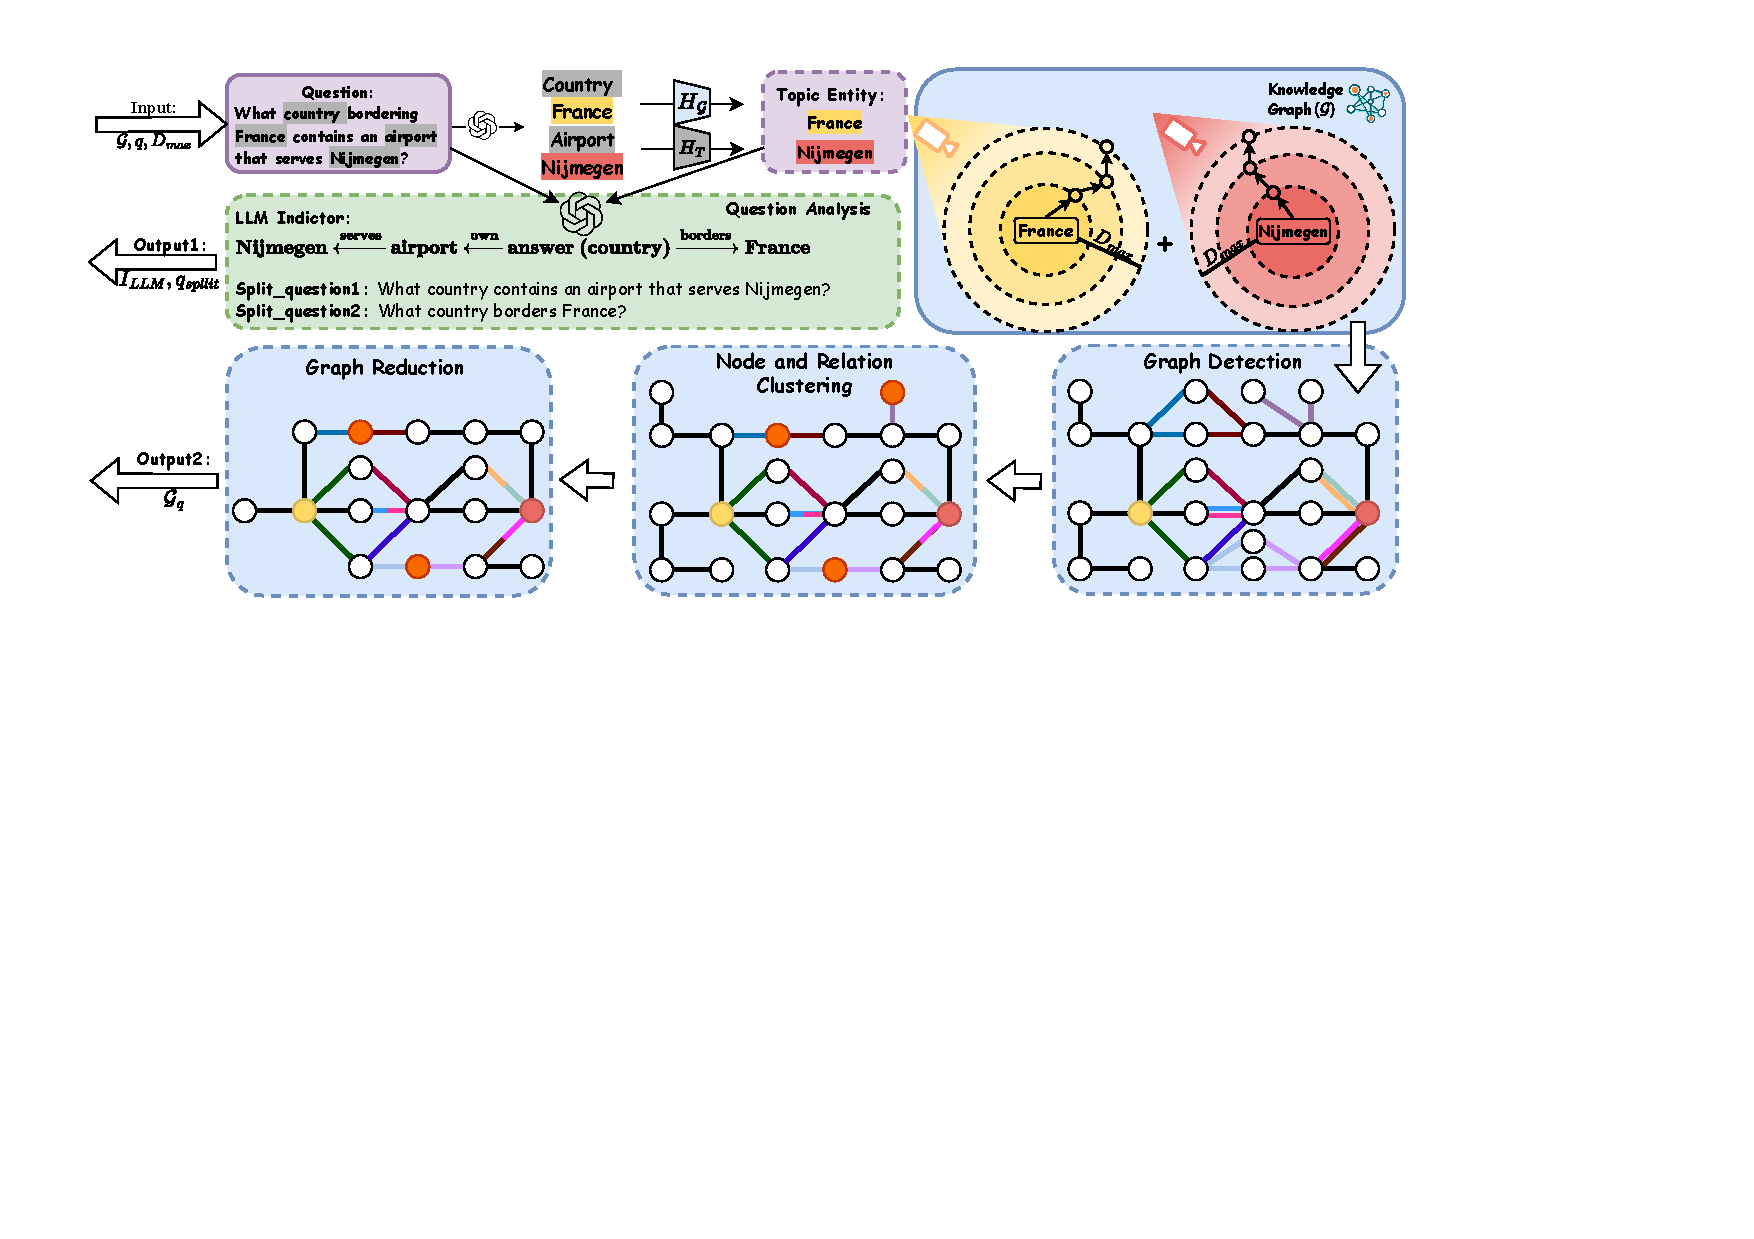
\includegraphics[width=1\linewidth]{graphs/Initiialization.pdf}
%     \caption{Caption}
%     \label{fig:enter-label}
% \end{figure}

% \begin{figure*}[!t]
%     \centering
%     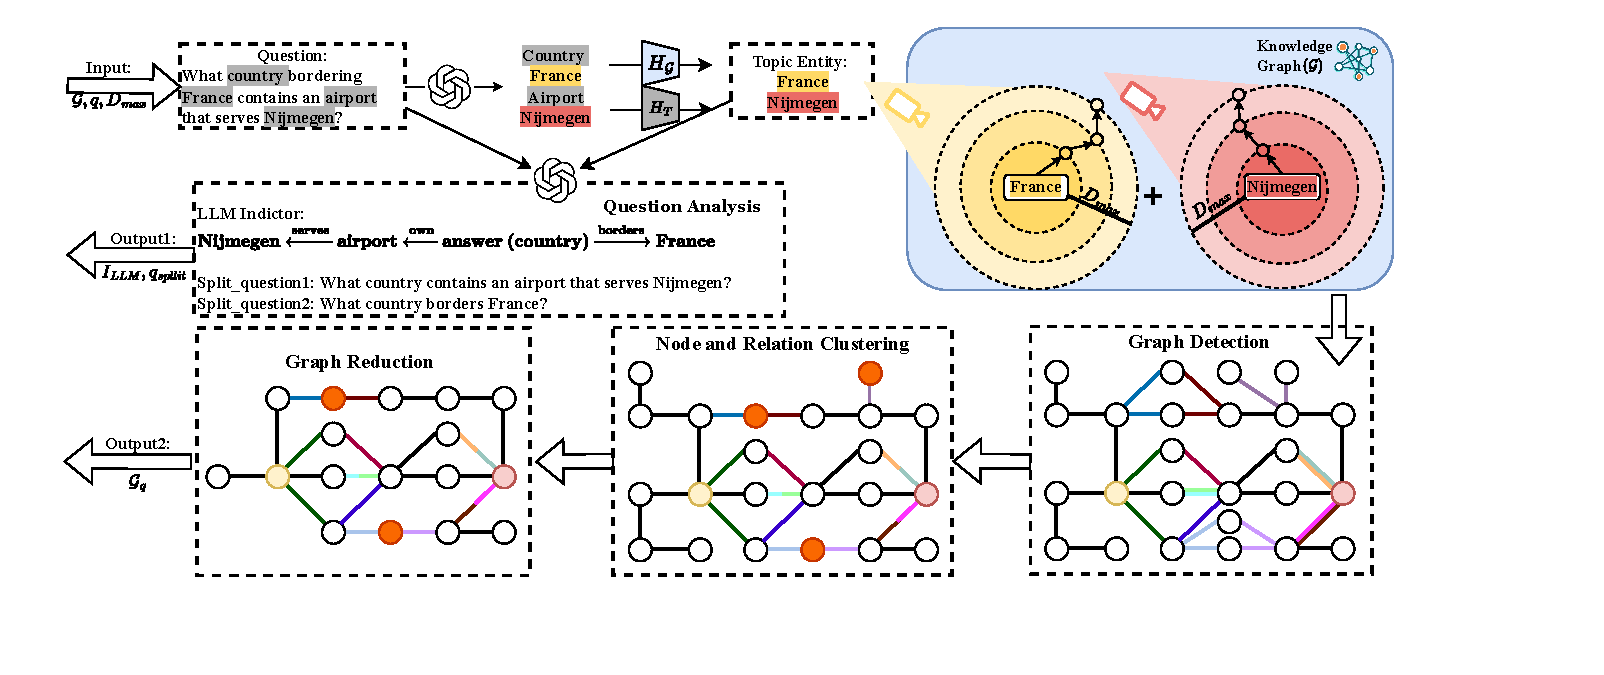
\includegraphics[width=\linewidth]{graphs/Initiialization_1.pdf}

%     \vspace{-1em}
% \end{figure*}

\begin{figure*}[t]
\centering
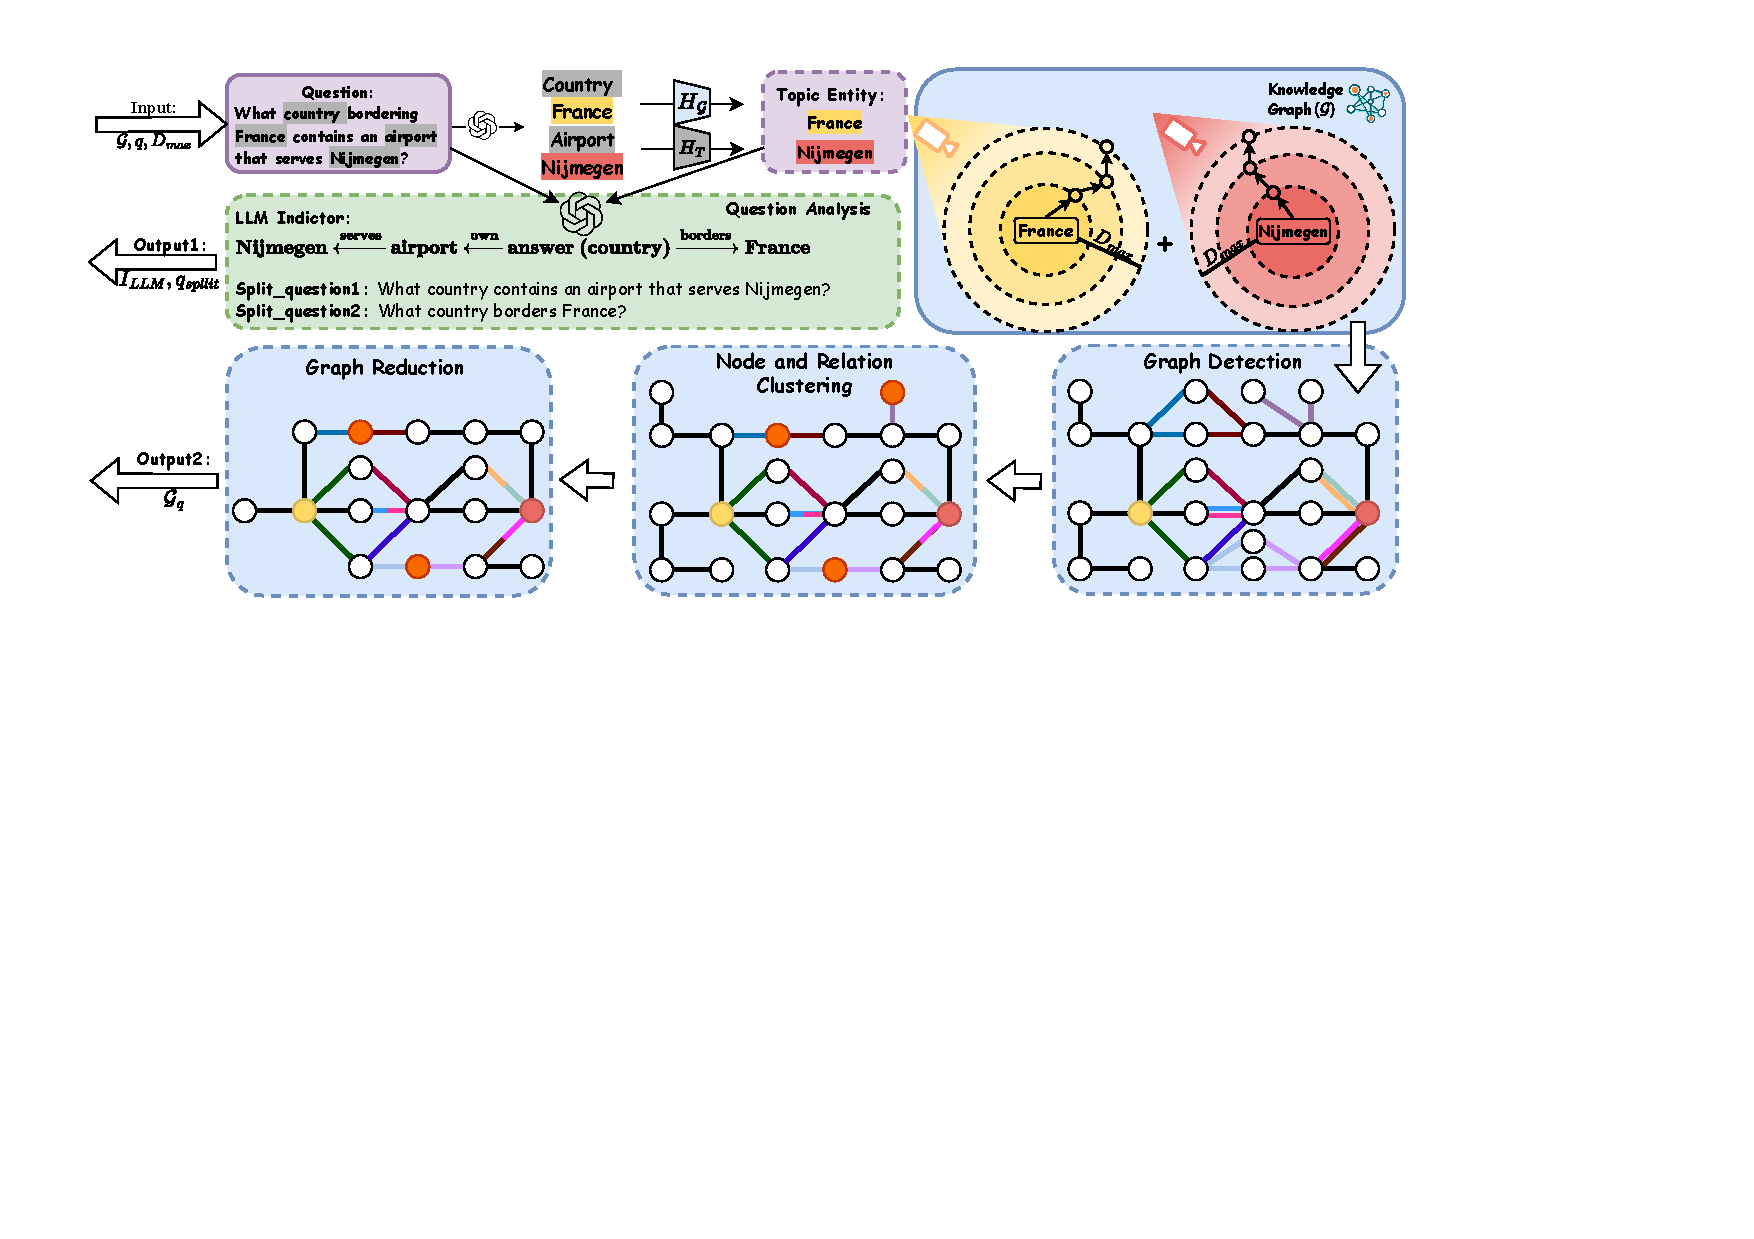
\includegraphics[width=0.9\linewidth]{graphs/Initiialization.pdf}
% \caption{Illustration of initialization.}
\caption{Overview of the initialization phase. 
% The initialization produces two key outputs. 
Output 1: from the input question, the model identifies topic entities and prompts the LLM to decompose questions into split questions $q_{split}$ and generate an indicator $I_{LLM}$. The indicator outlines a strategy for formulating the answer and predicts the exploration depth $D_{predict}$. Output 2: the model queries the source KG up to $D_{max}$-hop from identified topic entities, constructing and pruning the evidence subgraph $\mathcal{G}_q$. }
% Noted, In the pruning step, edges in different colors represent distinct relationships, and orange nodes or multi-colored edges indicate clustered nodes and edges.
\label{fig:initial}
\vspace{-1em}
\end{figure*}

\subsection{Initialization}
\label{method:initialization}

The initialization has two main stages, i.e., question subgraph detection and question analysis. The framework is shown in Figure~\ref{fig:initial}.

% \subsubsection{Question Subgraph detection}

% Given a question $q$,
% PoG first capture the question subgraph which contains all the topic entities of $q$ and their $D_{max}$-hops neighbors. 

% \myparagraph{Topic entity recognition} To capture the subgraph, PoG first prompts LLMs to extract the topic entities in question and gets the topic entities to the question. Then, applying BERT similarity to match entities and keywords. Specifically, we encode all the keyword entities extracted by LLM and all the entities $\mathcal{E}$ from the external knowledge graph into dense embeddings, and then compute the cosine similarity matrix between them. For each keyword, we obtain the entity set $Topic(q)$ with the highest similarity scores, which we use to build the evidence subgraph in the next step. 






% \subsubsection{Question Subgraph Detection}\label{method:1.1subgraphD}


\myparagraph{Question subgraph detection}
Given a question $q$, PoG initially identifies the question subgraph, which includes all the topic entities of $q$ and their $D_{\max}$-hop neighbors. 

\myparagraphunderline{Topic entity recognition}
To identify the relevant subgraph, PoG first employs LLMs to extract the potential topic entities from the question. Following the identification, the process applies BERT-based similarity matching to align these potential entities with entities from KG. Specifically, as shown in Figure \ref{fig:initial},
% we encode both the keywords identified by the LLMs and all entities $\mathcal{E}$ from the external knowledge graph 
we encode both the keywords and all entities from KG
into dense vector embeddings as $H_T$ and $H_{\mathcal{G}}$. We then compute a cosine similarity matrix between these embeddings to determine the matches. For each keyword, the entities with the highest similarity scores are selected to form the set $Topic(q)$. This set serves as the foundation for constructing the question subgraph in subsequent steps. 


% \myparagraph{Subgraph detection} After obtain the topic entities, PoG captures the induced subgraph $\mathcal{G}_q\subseteq\mathcal{G}$ by expanding each entity $e \in Topic(q)$. For entity $e$, it adds related knowledge triples by expanding its $D_{max}$-hops neighbors. 
% This approach incorporates query-related faithful KG information into $\mathcal{G}_q$. After exploration, we update $\mathcal{E}_q$ with newly added intermediate nodes from bridging pathways. 
% Finally, it forms the subgraph $\mathcal{G}_q = (\mathcal{E}_q, \mathcal{R}_q, \mathcal{T}_q)$ with $\mathcal{E}_q = Topic(q) \cup  \{N_\mathcal{G}(e, D_{max}) \mid e \in Topic(q)\}$.

\myparagraphunderline{Subgraph detection}
Upon identifying the topic entities, PoG captures the induced subgraph $\mathcal{G}_q \subseteq \mathcal{G}$ by expanding around each entity $e$ in $Topic(q)$. For each entity, we retrieve knowledge triples associated with its $D_{\max}$-hop neighbors, thereby incorporating query-relevant and faithful KG information into $\mathcal{G}_q$. Through this process, we update $\mathcal{E}_q$ with newly added intermediate nodes that serve as bridging pathways between the topic entities. The result subgraph, $\mathcal{G}_q$ is defined as $(\mathcal{E}_q, \mathcal{R}_q, \mathcal{T}_q)$, where $\mathcal{E}_q$ encompasses $Topic(q)$ together with the set $\{N_\mathcal{G}(e, D_{\max}) \mid e \in Topic(q)\}$, effectively linking all relevant entities and their connective paths within the defined hop distance. To interact with KG, we utilize the pre-defined SPARQL queries as detailed in Appendix \ref{appendix:aparql}.


% \myparagraph{Graph prune}To manage information overhead and reduce the cost of LLMs and searching space, we prune the $\mathcal{G}_q$ by graph compression in nodes' and relations' clustering and by graph reduction in Bidirectional BFS manner.
% By using bidirectional BFS, we find all paths linking all topic entities and regenerate new induced subgraphs with these paths. The purpose is to exclude all points that are not strongly related to topic entities in the generated subgraph, so that all the remaining points have a path connecting all topic entities and this point, and this path can be interpreted as the connection between this point and all topic entities through this reasoning path.
% These pruning steps result in the final question
% graph $\mathcal{G}_q$, optimizing information while preserving
% diversity and faithfulness. Specific algorithms details are shown in Appendix \textbf{TODO}.

% \myparagraphunderline{Graph pruning}
% To efficiently manage information overhead and minimize the computational cost associated with LLMs and search spaces, we implement graph pruning on $\mathcal{G}_q$ through node and relation clustering and graph reduction techniques. 
% As shown Figure \ref{fig:initial}, the node and relation clustering is realized by compress the node and relation, all the node that compressed denoted as a supernode that contains multiple node information, as well as the relation.
% For graph reduction, we utilize a bidirectional breadth-first search (bidirectional BFS) to identify all paths that link the topic entities, subsequently regenerating new induced subgraphs based solely on these paths. The aim of this approach is to exclude any points that do not have strong relevance to the topic entities. As a result, the remaining nodes in the pruned subgraph are those that not only have a direct path connecting them to all topic entities but also support the interpretation of their connection through these identified paths. This method of pruning ensures the final question graph $\mathcal{G}_q$ is optimized for relevant information while maintaining efficiency and faithfulness in the representation. 
% % Details of the specific algorithms used are provided in the Appendix \textbf{TODO}.

\myparagraphunderline{Graph pruning}
To efficiently manage information overhead and reduce computational cost, we implement graph pruning on the question subgraph $\mathcal{G}_q$ using node and relation clustering alongside graph reduction techniques.
As illustrated in Figure \ref{fig:initial}, node and relation clustering is achieved by compressing multiple nodes and their relations into supernodes, which aggregate information from the original entities and connections. 
For graph reduction, we employ bidirectional BFS to identify all paths connecting the topic entities. Based on these paths, we regenerate induced subgraphs that involve only the relevant connections, effectively excluding nodes and relations that lack strong relevance to the topic entities. 
% Consequently, the pruned subgraph $\mathcal{G}_q$ retains only those nodes that are directly connected to all topic entities and support the interpretability of their connections. This pruning strategy ensures that $\mathcal{G}_q$ is optimized for relevant information, maintaining both efficiency and faithfulness in its representation.



% \subsubsection{Question analysis}
% In order to reduce the hallucination of LLMs, in this phase, we prompt LLMs to process the question analysis in 2 parts in one LLM call with one example prompt. The first part is split the original question $q$. the prompt is designed to decompose the original complex question into serval simple question, based on the provided topic entities. For each entity, it will generate a simple question about how the relation between it and the answer.
% If LLMs can answer the splited question individually, then the original question can be answered. Hence, it is designed to reduce the hallucination. The second part is to generate a LLM indicator, which contains all the topic entities and answer in one reasoning path, based on the provide original question. The indicator can show the relationship between the topic entities and answer, and the order of all entities is matter. After obtaining the LLM indicator, we will use it to calculate a predict depth $D_{\text{predict}}$, which will be used in the exploration section for generate the reasoning path.
% \begin{example}
% given the question: "What country bordering France contains an airport that serves Nijmegen?", and topic entities: "{Nijmegen, France}". 
% The returned split questions are: 
% "What country contains an airport that serves "Nijmegen"?" and "split_question2: What country bordering "France"?"
% The LLM indicator is return as : "Nijmegen" - service by - airport - owned by - answer(country) - border with - "France", and the predict depth is 2 from each topic entity end.
% hence, the LLM indicator can shows show the relationship between the topic entities and answer, and the order also is another manifestation of relationship.


% \end{example}



% \subsubsection{Question Analysis}
% \label{method:1.2question_analysis}

% \myparagraph{Question analysis}
% To mitigate the hallucination effect often observed in LLMs, the question analysis phase is proposed and divided into two parts, executed within a single LLM call using an example-based prompt. The prompt template
% is detailed in Appendix \ref{appendix:prompt}.

% The first part involves splitting the original complex question $q$ into several simpler questions. This decomposition leverages the identified topic entities and formulates individual queries about their relations to the potential answer. If LLMs can address these simplified questions individually, then collectively, they provide a pathway to answer the original complex query, thereby reducing potential hallucinations.
% The second part entails generating an LLM indicator that encapsulates all topic entities and the answer within a single reasoning path, derived from the original question. This indicator illustrates the interrelations among the topic entities and the answer, emphasizing the significance of the sequence of entities. From this indicator, a predicted depth $D_{\text{predict}}$ is calculated, the depth is defined as the largest distance between predict answer and each topic entity.



\myparagraph{Question analysis}
To reduce hallucinations in LLMs, the question analysis phase is divided into two parts and executed within a single LLM call using an example-based prompt (shown in Appendix \ref{appendix:prompt}).
First, the complex question $q$ is decomposed into simpler questions based on the identified topic entities, each addressing their relationship to the potential answer. Addressing these simpler questions collectively guides the LLM to better answer the original query, thereby reducing hallucinations.
Second, a LLM indicator is generated, encapsulating all topic entities and predicting the answer position within a single chain of thought derived from the original question. This indicator highlights the relationships and sequence among the entities and answer. Based on this, a predicted depth $D_{\text{predict}}$ is calculated, defined as the maximum distance between the predicted answer and each topic entity.
An example of question analysis is shown in Figure \ref{fig:initial} with predicted depth 2.
% which is subsequently used in the exploration phase to generate the required reasoning path.

% \begin{example}
% \label{LLM_indictor}
% Consider the question: "What country bordering France contains an airport that serves Nijmegen?", with the topic entities: "{Nijmegen, France}". The process results in the following split questions:
% \begin{enumerate}
%     \item "What country contains an airport that serves Nijmegen?"
%     \item "What country borders France?"
% \end{enumerate}
% The LLM indicator is formulated as: 
% \[\text{"Nijmegen"} \xleftarrow{\text{serves}} \text{airport} \xleftarrow{\text{own}} \text{answer (country)} \xrightarrow{\text{borders}} \text{"France"},
% \]
% with a predicted depth of 2 from each topic entity end. This indicator not only clarifies the relationship between the topic entities and the answer but also signifies the importance of the order of entities in understanding their relationships.
% \end{example}







\vspace{-1pt}
\subsection{Exploration}
\label{method:exploration}



% As introduced in section \ref{method:1.2question_analysis}, it is very important to find a path that contains all topic entities. Each reasoning path is an interpretable form of the answer. You can consider a reasoning path as a chain of thoughts that may point to the answer. If this is a correct chain of thoughts, then the answer will be in this path. Similarly, this path also tells us how the answer should be obtained. In this article, it is defined as \textbf{interpretability}, because all paths that contain the correct answer essentially tell us how the answer is inferred.

% Therefore, maintainng efficiency and accuracy while obtaining the reasoning path is very important. In this section, it will be divided into three phases to obtain the path. After completing each phase, Path pruning and Question will be carried out, which will be introduced in following section. If the provided path is sufficient to answer the question, the process will be terminated, otherwise it will proceed to the next phase to obtain new reasoning paths.

% As discussed above, identifying a reasoning path that encompasses all topic entities is crucial. Each reasoning path serves as an interpretable sequence that potentially leads to the correct answer. These paths can be considered as chains of thoughts, and the answer might reside within them. 
% The sequence not only reveals the answer but also illustrates the method by which it is derived. In this paper, this clarity and traceability in the reasoning process are referred to as \textbf{interpretability}. Each valid path not only indicates the answer but also explicates the inferential steps leading to it.

As discussed in Section \ref{sec:1_intro}, identifying reasoning paths that encompass all topic entities is essential to derive accurate answers. These paths serve as interpretable chains of thought, providing both the answer and the inference steps leading to it, a feature we refer as \textbf{interpretability}.
% Ensuring both efficiency and accuracy in identifying these reasoning paths is paramount. The process in this section is structured into three phases to optimize the path discovery. After each phase, path pruning and question answering are conducted, details of which will be presented later. If a reasoning path obtained in any phase sufficiently answers the question, the process is concluded. Otherwise, the procedure advances to the next phase to explore additional reasoning paths.
To optimize the discovery of such paths efficiently and accurately, the exploration process is divided into three phases: topic entity path exploration, LLM supplement path exploration, and node expand exploration. After each phase, we perform path pruning and question answering. If a sufficient path is found, the process terminates; otherwise, it advances to the next phase to explore additional paths. 
Due to the space limitation, the pseudo-code of exploration section is shown in Appendix \ref{appendix:alg:explora}.


% \subsubsection{Topic entity path exploration}
% In order to reduce the LLM cost and searching space, we are not capture all the entity paths from max depth at beginning, in instead, for each question PoG will start from different predict depth $D_{predicr}$, which is obtained from section \ref{method:1.2question_analysis}.
% Given the provided Question subgraph $\mathcal{G}_q$, topic entity $Topic(q)$, LLM Indicator $I_{\text{LLM}}$, and predict depth $D_{\text{predict}}$ from section \ref{method:initialization}, PoG calculates all the reasoning paths containing all the topic entities by varying $D$ in each iteration.
% Before exploring paths, we sort $topic(q)$ in the same order with they occurs in $I_{\text{LLM}}$, as introduced in section \ref{method:1.2question_analysis}, the order of path does matter in the path resonning. 
% Then, with starting the iteration with $D=D_{\text{predict}}$,
% bidirectional BFS is utilized to obtain all the entity path $Topic_Path = {Path_{\mathcal{G}_q}(topic(q))}$ with length no exceeding $|Topic(q)|*D$. 
% To address the complexity of handling
% numerous entity path with the LLMs, we implement a 
% path pruning in following. 
% By passing the $Topic_Path$ and $I_{\text{LLM}}$, path pruning will narrow down the result into top-$W_{max}$ reasoning path,
% where $W_{max}$ is the width of beam search.
% And pruned $Topic_Path$ will be examined in Question answering section. If it is sufficient to answer the question, the process is terminated. Otherwise, the depth $D$ will expand one more, to capture more topic paths until the answer is given or $D$ exceeds $D_{max}$, then the next exploration phase will be processed.


% \begin{algorithm}[t]
% 	{
% 		{
% 			\SetVline
% 			\small
% 			\caption{{\small{Exploration and Reasoning}}}
            
% 			\Input{question subgraph ($\mathcal{G}_q$), question ($q$), split question ($q_{split}$), topic entities ($Topic(q)$), LLM indicator ($I_{\text{LLM}}$), predict depth ($D_{\text{predict}}$), maximum depth ($D_{max}$), and maximum width ($W_{max}$)}
% 			\Output{PoG answers ($a$), final reasoning path ($Final\_paths$)}
%             % \State{$T_d^+ \leftarrow$ Obtain positive $k$-truss with smallest query distance $d$ containing $Q$ in Algorithm~\ref{alg_local}}
%             % \setstretch{1.25}
%             \State{$List_{T} \leftarrow$ \text{Reorder}($Topic(q), I_{\text{LLM}}$)}
            
%             \textcolor{blue}{\tcc{Start with topic entity path exploration}}
            

%     % \State{\textbf{if} $Answer$ = True \textbf{then} \textbf{return} $Answer, Paths_{t}$ }

% \textcolor{blue}{\tcc{LLM supplement path exploration procedure}}

% \State{$Paths_s \leftarrow []$}

% \State{$ Predict(q) \leftarrow  $Sup\_Prediction($Paths_f, Q, I_{\text{LLM}}$)} 
% \ForEach{ $e,I_{sup(e)} \in Predict(q)$} {
%     \State{$List_{S} \leftarrow $ $List_{T} +e$ }
    
%     \State{$List_{S} \leftarrow $ Reorder ($List_{S}, I_{sup(e)}$)}
%     \State{$Paths_t \leftarrow \text{EntityPathFind}$ ($List_{S},D_{max}$,$\mathcal{G}_q$)}
%     \State{$Paths_s \leftarrow  Paths_s + \text{FuzzySelect}$ ($Paths_t, I_{sup(e)}, W_{max}$)}
%     }

%     \State{$Paths_{f} \leftarrow \text{PathsPruning}(Paths_s, Q, I_{\text{LLM}}, W_{max})$}
%     \State{$Answer, Paths_{s} \leftarrow \text{QuestionAnswering}(Paths_f, Q, I_{\text{LLM}})$}

%     % \State{$Answer, Paths_{s} \leftarrow \text{Reasoning}(Paths_s, Q, I_{\text{LLM}})$}
   
   


%     \State{\textbf{if} $Answer$ = True \textbf{then} \textbf{return} $Answer, Paths_{s}$ }
    

% \textcolor{blue}{\tcc{Node expand exploration procedure}}

%    \State{$Visted \leftarrow \emptyset$}
%    \State{$Paths_e \leftarrow Paths_{t} +Paths_{s} $}
%    \If{$|Paths_e| > W_{max}$} {
%    $Paths_e \leftarrow \text{PathsPruning}(Paths_e, Q, I_{\text{LLM}}, W_{max})$}

%    \State{$D\leftarrow1$}
%    \While{$D\leq D_{max}$} {
%     \State{$Entities \leftarrow$ ExtractEntity($Paths_e$)}
%     \ForEach{$e \in Entities \land e \notin Visted$} {
%         \State{$Related\_edges = \text{Find\_1\_hop\_Edges}(\mathcal{G}_q, e)$}
%         \State{$Paths_e = \text{MergeTogether}(Paths_e, Related\_edge)$}

        
%         % \State{$Visted = Visted \cup e$; $D\leftarrow D+1$}
%     }
%     \State{$Paths_{f} \leftarrow \text{PathsPruning}(Paths_e, Q, I_{\text{LLM}}, W_{max})$}
%     \State{$Answer, Paths_{e} \leftarrow \text{QuestionAnswering}(Paths_f, Q, I_{\text{LLM}})$}
%     % \State{\textbf{if} $Answer$ = True \textbf{then} \textbf{return} $Answer, Paths_{e}$ }
%     \State{\textbf{if}  $\{Yes\} \text{ in } Answer$  \textbf{then} \textbf{return} $Answer, Paths_{e}$;\\ \textbf{else} $Visted = Visted \cup e$; $D\leftarrow D+1$}
% }

%     \State{
%     $Paths_l \leftarrow Paths_T+Paths_S+Paths_E$
%     }
%     \State{
%     $Paths_l \leftarrow \text{PathsPruning}(Paths_l, Q, I_{\text{LLM}}, W_{max})$}
    
%     \State{$Answer,Paths_L \leftarrow \text{QuestionAnswering\_final}(Paths_l, Q, I_{\text{LLM}})$}
%     \State{\textbf{Return} $Answer,Paths_L$}

    
%     \textbf{Procedure}  topic\_entity\_path\_explor($D_{\text{predict}}, D_{max}, W_{max}$, $\mathcal{G}_q,Q, I_{\text{LLM}}, List_{T})$\\
%     \SetVline
%     \small
%     % \If{$v \neq Q$}{

%             \State{$D \leftarrow$ $D_{\text{predict}}$}
            
%             \While{ $D \leq D_{max}$} {
%                 \State{$Paths_t \leftarrow \text{EntityPathFind}$ ($List_{T},D$,$\mathcal{G}_q$)}
%                 \State{$Paths_{f} \leftarrow \text{PathsPruning}(Paths_t, Q, I_{\text{LLM}}, W_{max})$}
%                 \State{$Answer, Paths_{t} \leftarrow \text{QuestionAnswering}(Paths_f, Q, I_{\text{LLM}})$}

                
%                 \State{\textbf{if}  $\{Yes\} \text{ in } Answer$  \textbf{then} break;\\ \textbf{else} $D \leftarrow D + 1$}
% 			}
            
%             \State{\textbf{return} $Answer, Paths_{t}$}
% }
% }
% \end{algorithm}





% \subsubsection{Topic Entity Path Exploration}
% \label{method:2.1Entity_Path}

\myparagraph{Topic entity path exploration}
% To optimize the utilization of LLMs and reduce both the search space and associated costs, PoG initially does not capture all entity paths from the maximum depth. Instead, each question starts from a predicted depth $D_{\text{predict}}$, as determined in Section \ref{method:initialization}.
% This approach contrasts with previous methods (e.g.,  \cite{tog1.0sun2023think,tog2.0ma2024think}), which employ LLMs extensively to select neighboring entities for subgraph expansion. Our method can significantly reduce LLM cost by performing path explorations locally.
% Prior to exploring paths, we arrange the entities in $Topic(q)$ in the same sequence as they appear in $I_{\text{LLM}}$, as the order significantly impacts the reasoning process, as discussed in Section \ref{method:1.2question_analysis}. Starting the iterations at $D=D_{\text{predict}}$, bidirectional BFS is employed to derive all possible entity paths $Paths_{topic} = \{p \mid |Topic(q)| \times (D-1) < p \leq |Topic(q)| \times D\}$, where $p= Path_{\mathcal{G}_q}(topic(q))$ .
% Given the Question subgraph $\mathcal{G}_q$, the topic entities $Topic(q)$, the LLM indicator $I_{\text{LLM}}$, and the predicted depth $D_{\text{predict}}$ from Section \ref{method:initialization}, PoG systematically calculates all reasoning paths that incorporate all topic entities, adjusting the exploration depth $D$ in each iteration.
% Prior to exploring paths, we arrange the entities in $Topic(q)$ to match the sequence in which they appear in $I_{\text{LLM}}$. This ordering is crucial as it significantly influences the reasoning process, as elaborated in Section \ref{method:initialization}. Starting from the predicted depth $D=D_{\text{predict}}$, we employ a bidirectional BFS to derive all potential entity paths, which is defined as:
To reduce LLM usage and search space, PoG begins exploration from a predicted depth $D_{\text{predict}}$ rather than the maximum depth. Using the question subgraph $\mathcal{G}_q$, topic entities $Topic(q)$, LLM indicator $I_{\text{LLM}}$, and $D_{\text{predict}}$, PoG identifies reasoning paths containing all topic entities by iteratively adjusting the exploration depth $D$. Entities in $Topic(q)$ are ordered according to $I_{\text{LLM}}$ to facilitate reasoning effectively. Starting from the predicted depth $D=min(D_{\text{predict}}, D_{\text{max}})$, we employ a bidirectional BFS to derive all potential entity paths, which is defined as:
\[
Paths_{t}\hspace{-1pt}=\hspace{-1pt}\{p \mid |Topic(q)|\times (D-1) \hspace{-2pt}< \hspace{-2pt }length(p)\hspace{-2pt} \leq \hspace{-2pt}|Topic(q)| \times D\},
\]
% where $p = Path_{\mathcal{G}_q}(topic(q))$. This method ensures that the paths explored are within the specific bounds of the current depth increment, thereby focusing the search on a manageable subset of paths and improving the efficiency of the path exploration process.
% Due to the complexity of managing numerous entity paths with LLMs, a path pruning strategy is implemented. This strategy involves passing the $Paths_{topic}$ and $I_{\text{LLM}}$ through a process that narrows down the results to the top-$W_{max}$ reasoning paths, where $W_{max}$ is the beam search width. The pruned $Paths_{topic}$ is then evaluated in the Question Answering section. If it sufficiently answers the question, the process is terminated. Otherwise, the depth $D$ is incrementally expanded to capture more topic paths until the answer is obtained or $D$ exceeds $D_{max}$. Should these conditions be met without finding an answer, the exploration process advances to the next phase.
where $p = Path_{\mathcal{G}_q}(Topic(q))$. To reduce the complexity, a pruning strategy is employed and selects the top-$W_{\max}$ paths based on $Paths_{t}$, $I_{\text{LLM}}$, and split questions from Section \ref{method:initialization}. These paths are evaluated for sufficiency verification. If inadequate, $D$ is incremented until $D_{\max}$ is reached. Then the next phase commences.



% \subsubsection{LLM supplement path exploration}
% \label{method:2.2LLM_Path}

% We find that previous retrieval-augmented LLMs
% tend to rephrase the retrieved facts without exploiting the knowledge of LLM itself.
% Hence, in this section 
% we focus on not only relying on the pruned $Paths_{topic}$, but also promt LLM to make predictions based on the path understanding and its implicit knowledge. These predictions may be irrelevant to the existing acquired paths. Because we noticed that LLM can leverage its implicit knowledge to expand, connect, and improve the information relevant to the query. This ability is especially valuable when the external knowledge input is inaccurate. 
% When generating prediction results Predict(q), relative new LLM indicators $I_{\text{Sup}}$ are generated, which are similar to the previous $I_{\text{LLM}}$.
% for each predict entity $e\in Predict(q)$, 
% we utilize the text similarity to match the $e$ in $\mathcal{E}_q$, and form new Sup entity list $List_{S}(e) = Topic(p) + e$. the Sup entity list is reorder the $List_{S}(e)$ with new $I_{\text{Sup}}$. but generated the new supplement entity path $Sup\_paths$ with $D_{max}$ in stead of varying $D$, i.e., $Sup\_paths = \{p \mid length(p) \leq |Topic(q)| \times D\}$, where $p = Path_{\mathcal{G}_q}(List_{S}(e))$. 
% similarly to the section \ref{method:2.1Entity_Path}, the $Sup\_paths$ is pruned and examined in question answering section. 


% \subsubsection{LLM Supplement Path Exploration}
% \label{method:2.2LLM_Path}

\myparagraph{LLM supplement path exploration}
% Previous retrieval-augmented LLMs often tend to merely rephrase retrieved facts, failing to leverage the inherent knowledge of the LLM itself. To address this limitation, this section proposes a method that extends beyond relying solely on the pruned $Paths_{topic}$. 
% Instead, we prompt the LLM to make predictions based on its understanding of the path and its implicit knowledge, which may yield insights not directly related to the paths previously acquired. This capability of the LLM is particularly beneficial when the external reasoning results are inaccurate or incomplete.
% The method is realized in two parts, executed within a single LLM call using an example-based prompt. The prompt template is detailed in Appendix \ref{appendix:prompt}.
% \myparagraphunderline{Prompt-based LLM prediction}
% During the prediction phase, new LLM indicators $I_{\text{Sup}}$ are generated, akin to the earlier $I_{\text{LLM}}$. For each predicted entity $e \in Predict(q)$, we employ text similarity techniques to align $e$ with entities in $\mathcal{E}_q$. This leads to the formation of a new Sup entity list $List_{S}(e) = Topic(p) + e$. This list is then reordered according to the new $I_{\text{Sup}}$ indicators.
% \myparagraphunderline{LLM supplement path}
% Previous retrieval-augmented LLMs often merely rephrase retrieved facts without leveraging the inherent capabilities of the LLM. In contrast, PoG approach enables the LLM to synergistically infer from both the retrieved evidence graphs and its own knowledge base.
% Unlike the previous approach where $D$ was varied, the supplementary entity path $Sup\_paths$ is generated by filtering all paths in $\mathcal{G}_q$ using the maximum depth $D_{max}$, defined as:
Traditional KG-based LLM reasoning often rephrases KG facts without utilizing the LLM's inherent knowledge. To overcome this, PoG prompts LLMs to generate predictions based on path understanding and its implicit knowledge, providing additional relevant insights. 
It involves generating new LLM thinking indicators $I_{\text{Sup}}$ for predicted entities $e \in Predict(q)$, and then using text similarity to verify and align them with $\mathcal{E}_q \in \mathcal{G}_q$. 
The supplementary entity list $List_{S}(e) = Topic(q) + e$ is built and ranked by $I_{\text{Sup}}$ to facilitate reasoning effectively. Next, supplementary paths $Paths_{s}$ are derived from $List_{S}(e)$ in the evidence KG $\mathcal{G}_q$ with a fixed depth $D_{\max}$:
\[
Paths_{s} = \{ p \mid \text{length}(p) \leq |Topic(q)| \times D_{\max} \},
\]
where $p = Path_{\mathcal{G}_q}(List_{S}(e))$. These paths with new indicators
% undergo pruning and 
are evaluated similarly to the topic entity path exploration phase. The prompting temple is shown in Appendix \ref{appendix:prompt}.
% and detailed pseudocode is available in Appendix \ref{appendix:alg:explora}.



% \[
% Sup\_paths = \{p \mid \text{length}(p) \leq |Topic(q)| \times D\},
% \]
% where $p = Path_{\mathcal{G}_q}(List_{S}(e))$. Similar to topic entity path exploration, the paths within $Sup\_paths$ undergo pruning and are subsequently evaluated in the question-answering phase.


% \subsubsection{Node expand exploration}
% PoG processes the node exploration if the answer is not captured from previous exploration components.
% Compared to the existing work that explored in relation and entity speratly, we explore the both of relation and tail entity in form of knowledge triple. 
% Because the semantic information is clearer in the complete triple, it is easier to merge with the existing path to form a new path. At the same time, due to the previous graph reduction, we have reduced a lot of search space.
% In this section, the exploration can repeat at most $D_{max}$ times, for each time we explored the unvisited entity from the existing prunned path, denoted as $Existing\_paths = Paths_{topic} + Sup\_paths$, by 1-hop neighbor in the source KG $\mathcal{G}$. then the new explored triple will be mergeing into the existing path and graph, and generate new $Existing\_paths$.
% after each iteration, the new $Existing\_paths$ will undergo pruning and are subsequently evaluated in the question-answering phase. 
% the iteration will repeat until it reach the $D_max$ times or answer generated.

% \subsubsection{Node Expand Exploration}
% If the answer is not obtained from previous exploration phases, 
\myparagraph{Node expand exploration}
% If the pruned paths are not sufficient to answer the question from previous exploration phases, 
% the PoG method processes node exploration. Unlike existing methods that explore relations and entities separately, our approach explores both the relation and the tail entity simultaneously within the framework of a complete knowledge triple. This strategy benefits from the clearer semantic information provided by full triples, facilitating easier integration with existing paths to form new paths. Moreover, due to prior graph reduction efforts, the search space has already been substantially narrowed.
% In this phase, the exploration may repeat up to $D_{max}$ times. In each iteration, we explore unvisited entities from the existing pruned path, denoted as $Existing\_paths = Paths_{topic} + Sup\_paths$, extending outwards by 1-hop neighbors in the source Knowledge Graph $\mathcal{G}$. Newly discovered triples are then merged into the existing paths and graph to update the $Existing\_paths$.
% After each iteration, the updated $Existing\_paths$ undergoes further pruning and is evaluated during the question-answering phase. This iterative process repeats until either the exploration depth reaches $D_{max}$ or the answer is successfully generated.
If previous phases cannot yield sufficient paths, PoG proceeds to node expansion. Unlike previous methods \cite{tog1.0sun2023think,tog2.0ma2024think} that separately explore relations and entities, PoG explores both simultaneously, 
% within complete knowledge triples, 
leveraging clearer semantic information for easier integration with existing paths. 
During the exploration, PoG expands unvisited entities by 1-hop neighbors in $\mathcal{G}$. New triples are merged into existing paths to form the new paths, followed by pruning and evaluation. 
% This continues until $D_{\max}$ is reached or an answer is found.

% After each expand exploration, 

% $Existing\_paths = Paths_{topic} + Sup\_paths$, followed by pruning and evaluation. This continues until $D_{max}$ is reached or an answer is found.


\vspace{-1pt}
\subsection{Path Pruning}
\label{method:3pathprune}

% \begin{figure*}[!t]
%     \centering
%     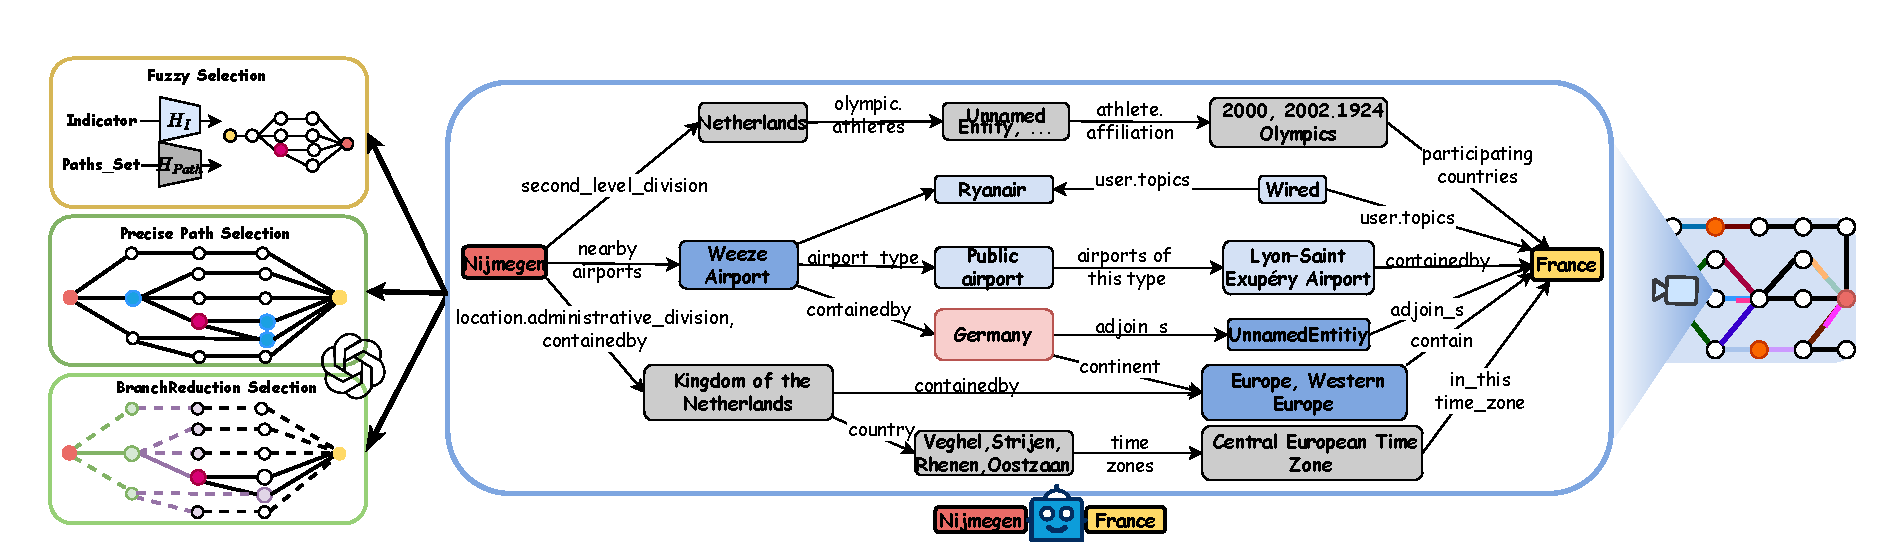
\includegraphics[width=\linewidth]{graphs/PathPrune.pdf}
%     \caption{The illustration of paths pruning.}

%     \vspace{-1em}
% \end{figure*}


As introduced in Section \ref{sec:related_work}, KGs contain vast amounts of facts,
making it impractical to involve all relevant triples in the LLM’s context due to high costs. To address this complexity and reduce LLM overhead, we utilize a three-step beam search for path pruning. The corresponding pseudo-code can be found in Appendix \ref{appendix:alg:pathpruning}.
% \subsubsection{Fuzzy Selection}

% \myparagraph{Fuzzy selection}
% Given the excessive volume of paths generated and the fact that only a small subset is likely relevant to the answer, the initial step in our beam search is fuzzy selection. This method is a non-LLM technique that aims to minimize additional computational overhead. For this purpose, we utilize SentenceBERT as a pruning tool to select the top-$W_1$ paths based on their literal similarities to the LLM indicator $I_{\text{LLM}}$.
% Specifically, we encode both the LLM indicator $I_{\text{LLM}}$ and all reasoning paths into dense vector embeddings. We then compute a cosine similarity matrix between these embeddings to determine their similarities. Ultimately, the paths with the highest top-$W_1$ similarity scores are selected for further processing. This step significantly reduces the number of paths that require evaluation by the LLM, thus lowering the overall computational demand.



\myparagraph{Fuzzy selection}
Considering that only a small subset of the generated paths is relevant,
the initial step of our beam search involves fuzzy selection by integrating a pre-trained language model (e.g. SentenceBERT \cite{reimers-gurevych-2019-sentence}), to filter the irrelevant paths quickly.
As shown in Figure \ref{fig:overall}, we encode the LLM indicator $I_{\text{LLM}}$ (or $I_{\text{Sup}}$) and all reasoning paths into vector embeddings, denoted as $H_I$ and $H_{Paths}$, and calculate cosine similarities between them. The top-$W_1$ paths with the highest similarity scores are  selected for further evaluation.
% \subsubsection{Precise Path Selection}

\myparagraph{Precise path selection}
Following the initial fuzzy selection, the number of candidate paths is reduced to $W_1$. At this stage, we prompt the LLM to select the top-$W_{\max}$ reasoning paths most likely to contain the correct answer. The specific prompt used to guide LLM in selection phase can be found in Appendix \ref{appendix:prompt}.

% \myparagraph{Branch reduced selection}
% Considering that the paths are represented in natural language and can sometimes be lengthy, resulting in high LLM processing costs, a branch reduction method by integrating the graph structure is utilized here to refine the path selection further. This method balances cost efficiency with accuracy in the final path selection.
% Starting from $D = 1$, for each entity in the entity list \ie $e\in list$, the method extracts the first $D$-step of $e$ from each path in the candidate set $Paths_c$ to the set $Paths_e$.
% If the number of $Paths_e$ exceeds the designated width $W_{max}$, these paths are pruned by precise path selection, and $Paths_c$ also be processed until the $|Paths_c| \leq D_{max}$.
% For example, in Figure \ref{fig:overall}, by setting $W_{max} = 1$, if we consider the red node only the first step is to extract the green paths, and the paths in dashed-line are pruned, for the next round, the path from orange to purple will be examed.
% Under the premise of ensuring the length and relevance of the reasoning path, Branch reduced selection achieves fast iterative selection with a small number of tokens.

% Based on the three path pruning methods, PoG supports various beam search strategies, ranging from non-reliant to fully reliant on LLMs, selectable in a user-friendly manner. We have defined the four strategies in Algorithm \ref{algorithm:PathsPruning}. 

\myparagraph{Branch reduced selection}
Considering that paths are often represented in natural language and can be extensive, leading to high processing costs for LLMs, we implement a branch reduced selection method integrated with the graph structure. This method effectively balances efficiency and accuracy by further refining path selection. Starting with $D = 1$, for each entity $e$ in the entity list, we extract the initial $D$-step paths from every path in the candidate set $Paths_c$ into a new set $Paths_e$. If the number of $Paths_e$ exceeds the maximum designated width $W_{\max}$, these paths are pruned using precise path selection. The process iterates until the number of paths in $Paths_c$ reaches $D_{\max}$. For example, as illustrated in Figure \ref{fig:overall}, with $W_{\max} = 1$, only the initial step paths (depicted in green) are extracted for further examination, while paths represented by dashed lines are pruned. This selection method enables efficient iterative selection by limiting the number of tokens and ensuring the relevance and conciseness of the reasoning paths.



\myparagraph{Beam search strategy}
Based on the three path pruning methods above,
% —fuzzy selection, precise path selection, and branch reduced selection—
PoG can support various beam search strategies, ranging from non-reliant to fully reliant on LLMs. These strategies are selectable in a user-friendly manner, allowing flexibility based on the specific requirements of the task. We have defined four such strategies in Algorithm \ref{algorithm:PathsPruning} of Appendix \ref{appendix:alg:pathpruning}. 



% \myparagraph{Branch Reduced Selection}
% Given that paths can be verbose and lead to high LLM processing costs, we implement a branch reduction method integrating graph structure to refine path selection efficiently. This method balances cost efficiency with accuracy in final path selection. The process starts with each entity $e \in \text{list}$, setting $D = 1$ to extract the first-step of $e$ from each path in the candidate set $Paths_c$ to the set $Paths_e$. If $Paths_e$ exceeds the designated width $W_{max}$, these paths undergo Precise Path Selection to narrow them down to $W_{max}$. Only selected $Paths_e$ and their corresponding original paths are retained; unselected paths are removed from $Paths_c$.

% If $Paths_c$ still exceeds $W_{max}$ after the first step, $D$ is incremented by one, and the process of extraction and selection repeats. This cycle continues until the quantity of $Paths_c$ aligns with width requirements. Ultimately, the refined $Paths_c$ are returned for further processing, ensuring that branch reduced selection achieves fast, iterative selection with minimal tokens.

% The three path pruning methods allow PoG to support various beam search strategies, ranging from non-reliant to fully reliant on LLMs, as outlined in Algorithm \ref{algorithm:PathsPruning}.

% \subsection{Question answering}

% We find that previous retrieval-augmented LLMs
% tend to rephrase the retrieved facts without exploiting the knowledge of LLM itself. However,
% PoG enables LLM to synergistically infer
% from both the retrieved evidence graphs and its
% own knowledge. We attribute this ability to three
% aspects: 
% (1) Language Understanding, as LLM can
% comprehend and extract the knowledge from provided knowledge paths
% and the query in natural language, 
% (2) Knowledge Reasoning, as LLM can perform entity disambiguation and produce the final answer based on the provided finial knowledge paths, and (3) Knowledge Enhancement, as LLM can leverage its implicit knowledge to expand, connect, and improve the information relevant to the query. This ability is especially valuable when the external knowledge input is incomplete.

% Based on the three keys, we proposed our question answering method by 2 steps.
% \myparagraph{Path summarizing}

% Because some paths have too much text information, in some cases, even if the text information provided is wrong, LLM will answer the wrong question or provide the correct path, but the answer will be wrong. In order to solve this illusion problem, we proposed a strategy of summarizing the path first and then answering the question.

% Through the LLM prompt, by thinking about the provided path and split question, the triples related to the split question are extracted from the path and a new path is formed.
% The specific prompt used to guide the LLM in this selection process is detailed in the Appendix \textbf{TODO}.


% \myparagraph{Question Answering}
% we prompt LLMs to evaluate the provide answer if can answer all the split question first, then if can answer the original question.
% if both yes, the answer will be extraction from the provided path. all the process in this section is only call LLM once.

% if the node exploration reach the last depth and still no answer generated, we prompt LLM to answer the question by both provided knowledge and its inherited knowledge.The specific prompt used to guide the LLM in this selection process is detailed in the Appendix \textbf{TODO}.






\vspace{-1pt}
\subsection{Question Answering}
% This enhanced functionality is attributed to three main aspects:
% \begin{enumerate}
%     \item \textbf{Language Understanding}: LLMs can comprehend and extract knowledge from the provided knowledge paths and queries expressed in natural language.
%     \item \textbf{Knowledge Reasoning}: LLMs are capable of performing entity disambiguation and deriving the final answer from the final knowledge paths provided.
%     \item \textbf{Knowledge Enhancement}: LLMs can utilize their implicit knowledge to expand, connect, and refine the information pertinent to the query, which is invaluable when the external knowledge inputs are incomplete.
% \end{enumerate}
Based on the pruned paths in Section \ref{method:3pathprune}, we introduce a two-step question-answering method.

% \subsubsection{Path Summarizing}
% \myparagraph{Path summarizing}
% To address the issue of paths containing excessive or incorrect text information, which can lead to incorrect responses, we propose a strategy that involves summarizing the path before answering the question. Using an LLM prompt, the model thinks through the provided path and split question, extracting triples related to the split question to form a new, concise path. The specifics of the prompt used in this process are detailed in the Appendix \ref{appendix:prompt}.

% % \subsubsection{Question Answering}
% \myparagraph{Question answering}
% In this stage, we prompt the LLM to evaluate whether the provided answers can address all the split questions and then determine whether they can adequately respond to the original question. If both conditions are satisfied, the answer is extracted from the path provided and generated by prompting LLMs. 
% If the node exploration reaches the last permissible depth without generating an answer, we prompt the LLM to derive the answer using both the provided knowledge and its inherent knowledge. Details regarding the prompt used in this process are also specified in the Appendix \ref{appendix:prompt}.
\myparagraph{Path Summarizing}
To address hallucinations caused by paths with excessive or incorrect text, we develop a summarization strategy by prompting LLM to review and extract relevant triples from provided paths, creating a concise and focused path. Details of the prompts used are in Appendix \ref{appendix:prompt}.

% To address the issue of paths containing excessive or incorrect text information, which can lead to incorrect responses, we propose a strategy that involves summarizing the path before answering the question. Using an LLM prompt, the model thinks through the provided path and split question, extracting triples related to the split question to form a new, concise path. The specifics of the prompt used in this process are detailed in the Appendix \ref{appendix:prompt}.

\myparagraph{Question answering}
Based on the current reasoning path derived from path pruning and summarizing, we prompt the LLM to first evaluate whether the paths are sufficient for answering the split question and then the main question. If the evaluation is positive, LLM is prompted to generate the answer using these paths, along with the question and question analysis results as inputs, as shown in Figures \ref{fig:overall}. The prompts for evaluation and generation are detailed in Appendix \ref{appendix:prompt}. If the evaluation is negative, the exploration process is repeated until completion. If node expand exploration reaches its depth limit without yielding a satisfactory answer, LLM will leverage both provided and inherent knowledge to formulate a response. Additional details on the prompts can be found in Appendix \ref{appendix:prompt}.



% \vspace{-1pt}
\section{Experiments}


% \setlength{\textfloatsep}{3pt}  % 表格与上下文的距离
% \setlength{\intextsep}{3pt} 
% {figure*}[!t]
% \tabcolsep{1.0 pt}
% \resizebox{}{!}{ 
\begin{table*}[t]
% Please add the following required packages to your document preamble:
% \usepackage{multirow}
% Please add the following required packages to your document preamble:

% Please add the following required packages to your document preamble:
% \usepackage{booktabs}
% \usepackage[normalem]{ulem}
% \useunder{\uline}{\ul}{}
% \small
\caption{Results of PoG across various datasets, compared with the state-of-the-art (SOTA) in Supervised Learning (SL) and In-Context Learning (ICL) methods. The highest scores for ICL methods are highlighted in bold, while the second-best results are underlined. The Prior FT (Fine-tuned) SOTA includes the best-known results achieved through supervised learning.}
\label{figure:mainresult}
\begin{tabular}{@{}cccccccc@{}}
\toprule
Method        & Class & LLM           & \multicolumn{3}{c}{Multi-Hop KGQA}   & Single-Hop KGQA  & Open-Domain QA \\ \cmidrule(lr){4-6}
              &       &               & CWQ  & WebQSP        & GrailQA       & Simple Questions & WebQuestions   \\ \midrule
\multicolumn{8}{c}{\textit{Without external knowledge}}                                                                   \\\midrule
IO prompt\cite{tog1.0sun2023think}     & -     & GPT-3.5-Turbo & 37.6 & 63.3          & 29.4          & 20.0               & 48.7           \\
CoT\cite{tog1.0sun2023think}            & -     & GPT-3.5-Turbo & 38.8 & 62.2          & 28.1          & 20.3             & 48.5           \\
SC\cite{tog1.0sun2023think}             & -     & GPT-3.5-Turbo & 45.4 & 61.1          & 29.6          & 18.9             & 50.3           \\ \midrule
\multicolumn{8}{c}{\textit{With external knowledge}}                                                                      \\ \midrule
Prior FT SOTA & SL    & -             & 70.4\cite{das2021case} & 85.7\cite{rogluo2023reasoning}          & 75.4\cite{gu2022don}          & 85.8\cite{baek2023direct}           & 56.3\cite{kedia-etal-2022-fie}           \\ \midrule
KB-BINDER\cite{li-etal-2023-shot}     & ICL   & Codex         & -    & 74.4          & 58.5          & -                & -              \\
ToG/ToG-R\cite{tog1.0sun2023think}     & ICL   & GPT-3.5-Turbo & 58.9 & 76.2          & 68.7          & 53.6             & 54.5           \\
ToG-2.0\cite{tog2.0ma2024think}       & ICL   & GPT-3.5-Turbo & -    & 81.1         & -             & -                & -              \\
ToG/ToG-R\cite{tog1.0sun2023think}     & ICL   & GPT-4         & 69.5 & 82.6          & 81.4          & 66.7             & 57.9           \\ \midrule
PoG-E         & ICL   & GPT-3.5-Turbo & 71.9 & 90.9          & 87.6          & 78.3             & 76.9           \\
PoG           & ICL   & GPT-3.5-Turbo & 74.7 & 93.9          & {\ul 91.6}          & 80.8             & 81.8           \\
PoG-E         & ICL   & GPT-4         & {\ul78.5} & {\ul 95.4}    & 91.4    & {\ul 81.2}       & {\ul 82.0}       \\
PoG           & ICL   & GPT-4         & \textbf{81.4} & \textbf{96.7} & \textbf{94.4} & \textbf{84.0}      & \textbf{84.6}  \\ \bottomrule
\end{tabular}


% 
% \vspace{-1em}
% \caption{The PoG results for different datasets compared with previous SOTA Supervised Learning (SL) and In-Context Learning based methods. The best
% results for ICL methods are marked in bold, the second results shown in underline. The prior FT (Fine-tuned) SOTA
% includes the best-known results.}
\end{table*}
% }



% \subsection{Experimental Settings}

% \myparagraph{Experimental Settings} To evaluate PoG's capability in multi-hop knowledge-intensive reasoning tasks, we assess it on five datasets: CWQ, WebQSP, GrailQA, SimpleQuestions, and WebQuestions comparing with the method without external Knwowldeg: IO, SC, CoT, and with previous SOTA among all prompting-based methods, fine-tuning based and all the method respectively.
% Freebase serves as the background knowledge graph for all datasets. 
% The experiment is conduct with two LLMs: ChatGPT and GPT-4.
% Following previous works, we use exact match accuracy (Hits@1) as our evaluation metric for all datasets.
% More experimental settings about dataset statistics, baselines, and implementation details are reported in \ref{appen:dataset_details}.

\myparagraph{Experimental settings}
We evaluate PoG on five KGQA datasets, i.e., CWQ \cite{talmor-berant-2018-web}, WebQSP \cite{yih-etal-2016-value}, GrailQA \cite{grailqa}, SimpleQuestions \cite{simplequestions}, and WebQuestions \cite{berant-etal-2013-semantic}. PoG is tested against methods without external knowledge (IO, CoT\cite{wei2022cot}, SC\cite{wang2022self}) and the state-of-the-art (SOTA) approaches with external knowledge, including prompting-based and fine-tuning-based methods. Freebase \cite{freebase} serves as the background knowledge graph for all datasets. Experiments are conducted using two LLMs, i.e., GPT-3.5 (GPT-3.5-Turbo) and GPT-4. Following prior studies, we use exact match accuracy (Hits@1) as the evaluation metric. Due to the space limitation, detailed experimental settings, including dataset statistics, baselines, and implementation details, are provided in Appendix \ref{appen:dataset_details}.



\myparagraph{PoG setting}
We adopt the \texttt{Fuzzy + Precise Path Selection} strategy in Algorithm \ref{algorithm:PathsPruning} of Appendix \ref{appendix:alg:pathpruning} for PoG, with $W_1 = 80$ for fuzzy selection. Additionally, we introduce \textbf{PoG-E}, which randomly selects one relation from each edge in the clustered question subgraph to evaluate the impact of graph structure on KG-based LLM reasoning. $W_{\max}$ and $D_{\max}$ are 3 by default for beam search.



\vspace{-1pt}
\subsection{Main Results}
Since PoG leverages external knowledge to enhance LLM reasoning, we first compare it with other methods that utilize external knowledge. 
% As we can see in Table \ref{figure:mainresult}, despite being a training-free, prompting-based method—which naturally places it at a disadvantage compared to fine-tuned methods trained on evaluation data-PoG with GPT-3.5-Turbo still achieves new SOTA performance across most datasets.
Although PoG is a training-free, prompting-based method and has natural disadvantages compared to fine-tuned methods trained on evaluation data.
As shown in Table \ref{figure:mainresult}, PoG with GPT-3.5-Turbo still achieves new SOTA performance across most datasets. 
% As shown in Table \ref{figure:mainresult}, PoG with GPT-3.5-Turbo achieves new SOTA performance across most datasets. This is an excellent result as a training-free, prompting-based method, which naturally places it at a disadvantage compared to fine-tuned methods trained on evaluation data.
Additionally, PoG with GPT-4 surpasses fine-tuned SOTA across all the multi-hop and open-domain datasets by an average of 17.3\% and up to 28.3\% on the WebQuestions dataset.
Comparing all the in-context learning (ICL) methods, 
PoG with GPT-3.5-Turbo surpasses all the previous SOTA methods. 
When comparing PoG with GPT-3.5-Turbo against SOTA using GPT-4, PoG outperforms the SOTA by an average of 12.9\% and up to 23.9\%. 
When using the same LLM, PoG demonstrates substantial improvements: 
with GPT-3.5-Turbo, it outperforms SOTA by an average of 21.2\% and up to 27.3\% on the WebQuestions dataset;
with GPT-4, it outperforms SOTA by 16.6\% on average and up to 26.7\% on the WebQuestions dataset.
Additionally, PoG with GPT-3.5-Turbo outperforms methods without external knowledge (e.g., IO, CoT, SC prompting) by 62\% on GrailQA and 60.5\% on Simple Questions. These results show that incorporating external knowledge graphs significantly enhances reasoning tasks.
PoG-E also achieves excellent results. Under GPT-4, PoG-E surpasses all SOTA in ICL by 14.1\% on average and up to 24.1\% on the WebQuestions dataset. These findings demonstrate that the graph structure is crucial for reasoning tasks, particularly for complex logical reasoning. By integrating the structural information of the question within the graph, PoG enhances the deep reasoning capabilities of LLMs, leading to superior performance.
% \vspace{-1pt}
\subsection{Ablation Study}\label{exp:ablation}
We perform various ablation studies to understand the importance of different factors in PoG. 
% The ablation studies are conducted with GPT-3.5-Turbo on two subsets of the test sets of CWQ and WebQSP, each of which contains 500 randomly sampled questions.
These ablation studies are performed with GPT-3.5-Turbo on two subsets of the CWQ and WebQSP test sets, each containing 500 randomly sampled questions.
\newline
\myparagraphquestion{Does search depth matter} As described, PoG's dynamic deep search is limited by $D_{max}$. 
To assess the impact of $D_{\max}$ on performance, we conduct experiments with depth from 1 to 4. The results, shown in Figures \ref{fig:ablation:depth}(a) and (c), indicate that performance improves with increased depth, but the benefits diminish beyond a depth of 3. 
Figures \ref{fig:ablation:depth}(b) and (d), showing which exploration phase the answer is generated from, reveal that higher depths reduce the effectiveness of both LLM-based path supplementation and node exploration. 
Excessive depth leads to LLM hallucinations and difficulties in managing long reasoning paths.
Therefore, we set the maximum depth to 3 for experiments to balance performance and computational efficiency.
Additionally, even at lower depths, PoG maintains strong performance by effectively combining the LLM's inherent knowledge with the structured information from the KG.
\begin{figure}[t]
    % \centering
    \begin{subfigure}{0.48\linewidth}
           \centering
           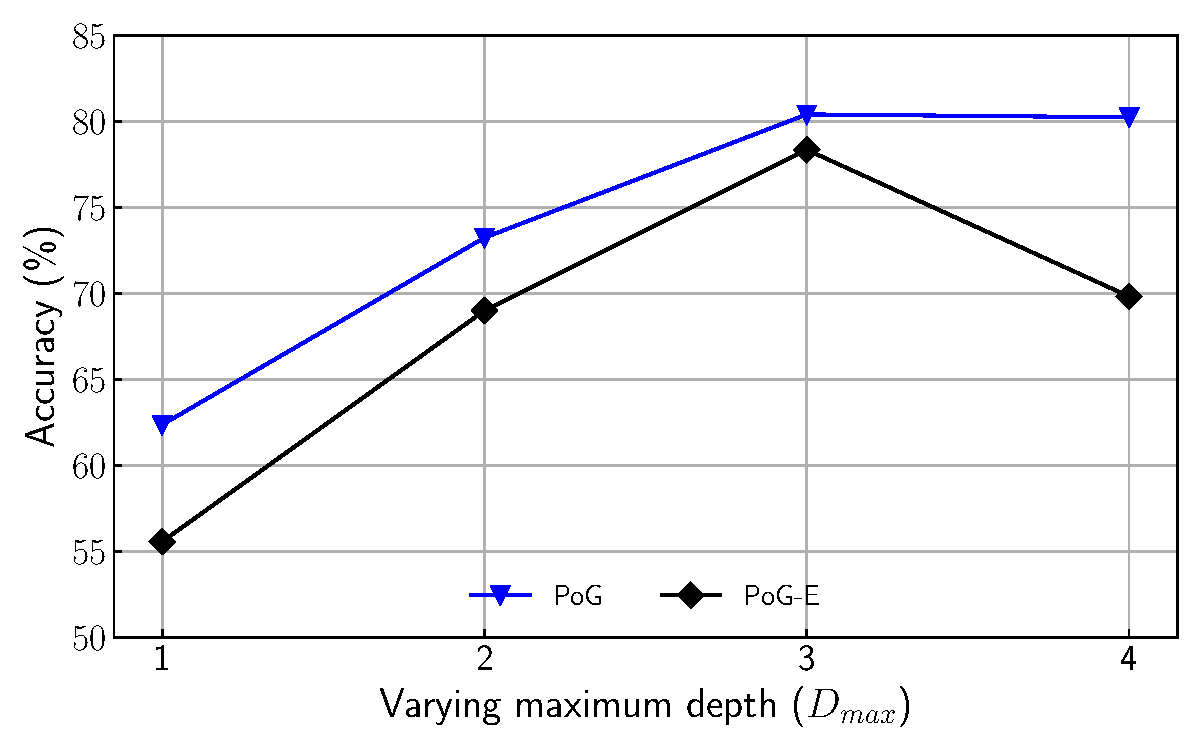
\includegraphics[width=1\linewidth]{graphs/acc_by_depth_cwq.pdf}
           % \vspace{-1mm}
           \caption{CWQ (Vary $D_{\max}$)}
            \label{fig:a}
    \end{subfigure}
    \begin{subfigure}{0.48\linewidth}
           \centering
           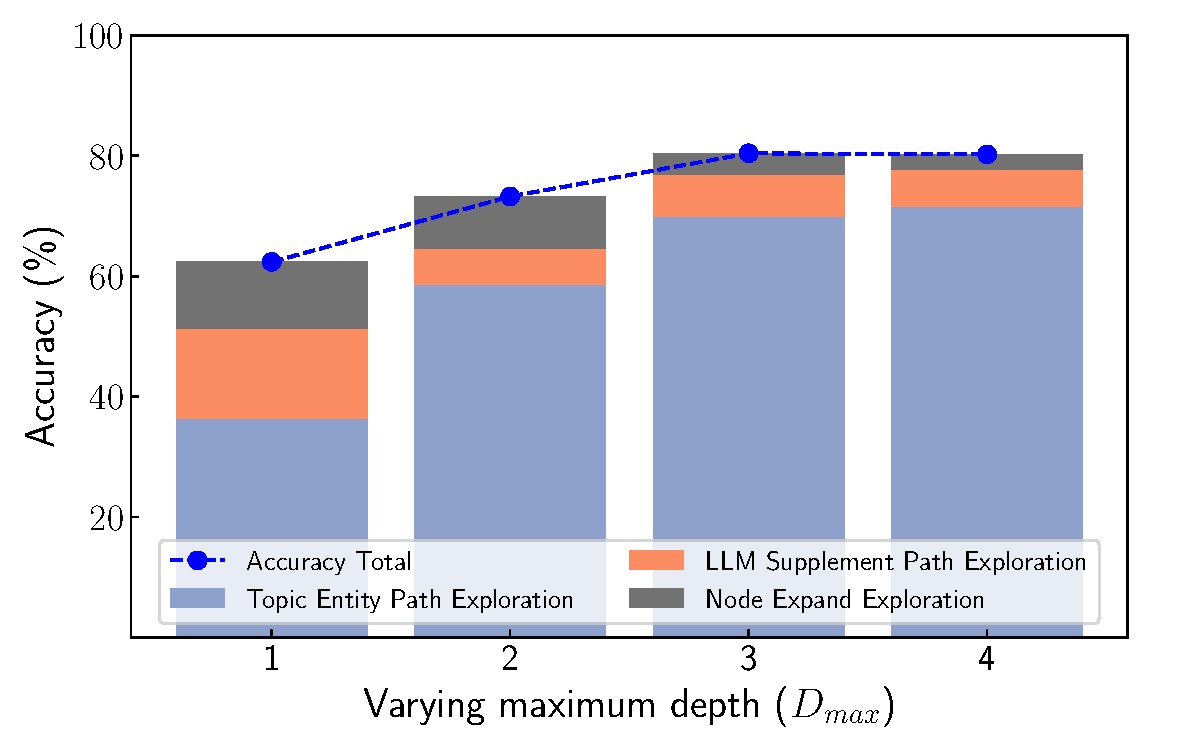
\includegraphics[width=1\linewidth]{graphs/acc_by_dep_cwq_pog.pdf}
           % \vspace{-1mm}
           \caption{CWQ(PoG)}
            \label{fig:b}
    \end{subfigure}
    \begin{subfigure}{0.48\linewidth}
           \centering
           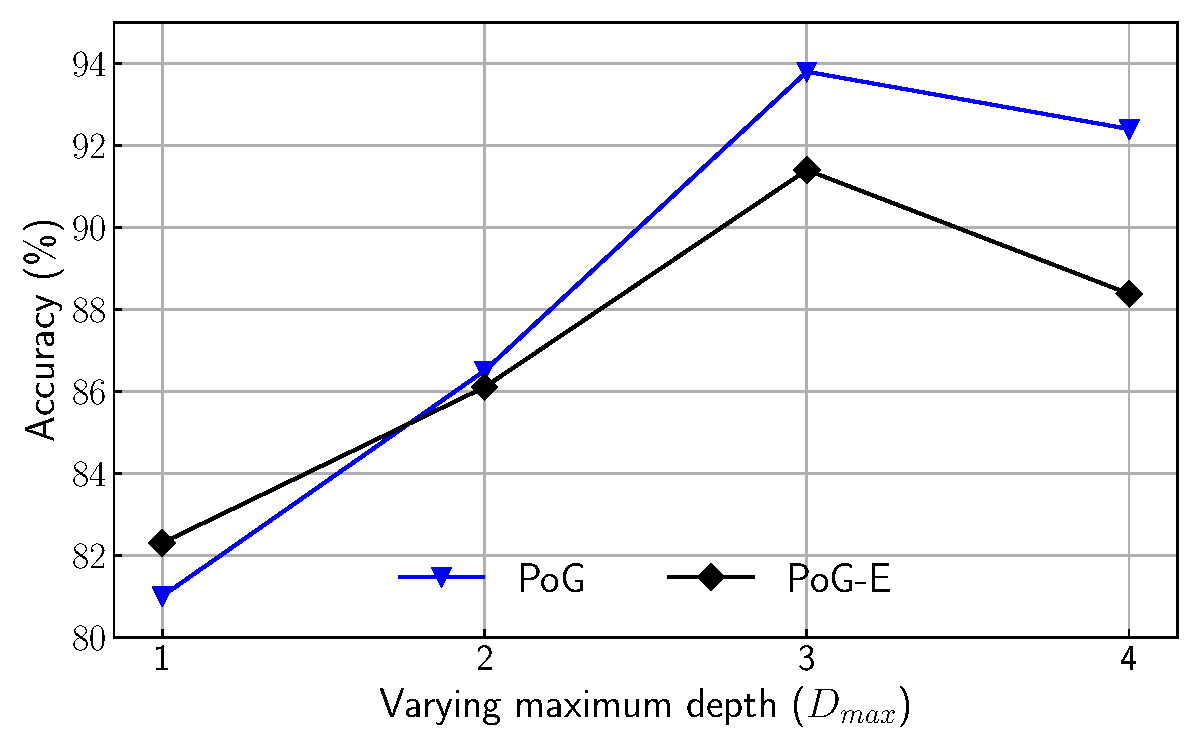
\includegraphics[width=1\linewidth]{graphs/acc_by_depth_webqsp.pdf}
           % \vspace{-1mm}
           \caption{WebQSP (Vary $D_{\max}$)}
            \label{fig:c}
    \end{subfigure}
    \begin{subfigure}{0.48\linewidth}
           \centering
           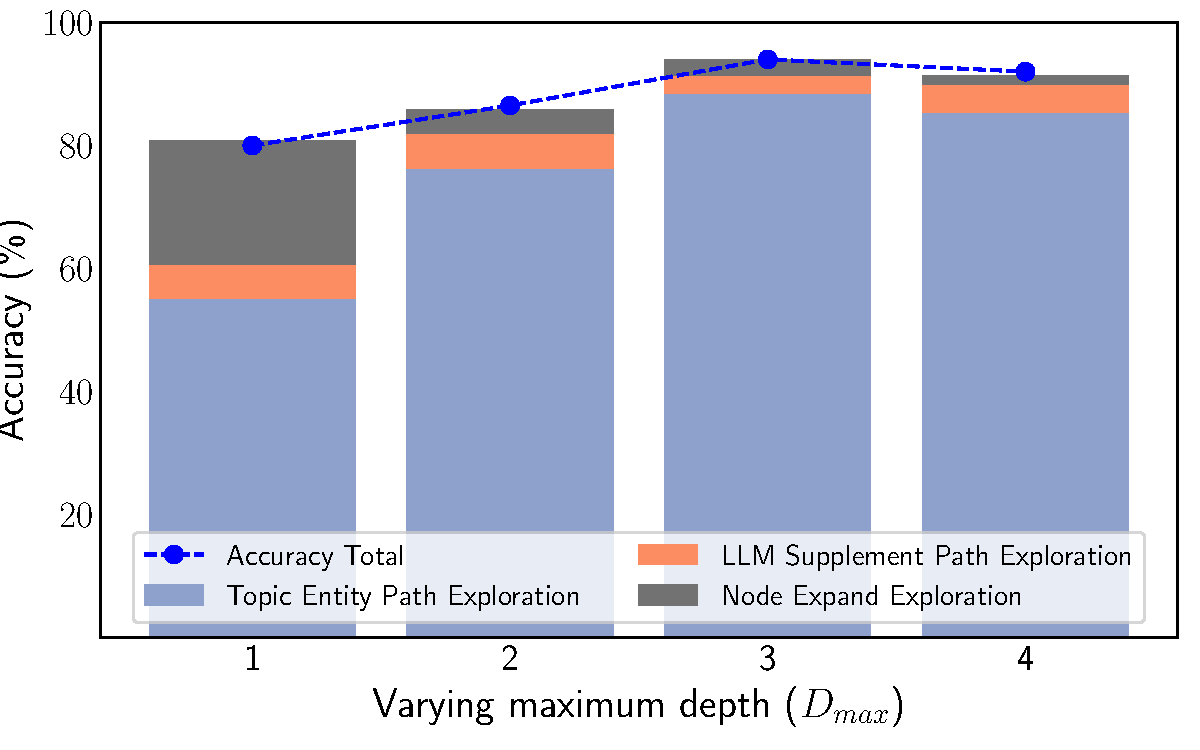
\includegraphics[width=1\linewidth]{graphs/acc_by_dep_webqsp_pog.pdf}
           % \vspace{-1mm}
           \caption{WebQSP(PoG)}
            \label{fig:d}
    \end{subfigure}
\vspace{-2mm}
\caption{The accuracy of PoG and PoG-E among CWQ and WebQSP datasets by varying different $D_{\max}$.}\label{fig:ablation:depth}
\vspace{-1mm}
\end{figure}
\subsection{Effectiveness Evaluation}\label{exp:result_analysis}
\myparagraph{Effective evaluation on multi-entity questions}
To evaluate PoG's performance on multi-entity questions, we report the accuracy on all test sets by categorizing questions based on the number of topic entities. The results, shown in Table \ref{fig:exp:mult_e}, demonstrate that, despite the increased complexity of multi-entity questions compared to single-entity ones, PoG maintains excellent accuracy, achieving up to 93.9\% on the WebQSP dataset. This underscores the effectiveness of our structure-based model in handling complex multi-entity queries. 
Notably, the slightly lower performance on the GrailQA dataset can be attributed to some questions lacking matched topic entities, which prevents effective reasoning using KG. 
% Please add the following required packages to your document preamble:
% \usepackage{booktabs}
\begin{table}[t]
% \vspace{-3mm} 
\caption{Performance of PoG and PoG-E on multi-entity and single-entity questions of all datasets. The symbol `-' indicates no multi-entity question inside.}\label{fig:exp:mult_e}
\setlength\tabcolsep{1.0 pt}
\resizebox{\linewidth}{!}{ 
\begin{tabular}{@{}lccccc@{}}
\toprule
      {\textbf{Question Set}}    & \multicolumn{1}{l}{\textbf{CWQ}} & \textbf{WebQSP}      & \textbf{GrailQA}     & \textbf{WebQuestions}  & \textbf{Simple Questions}\\ \midrule
\textbf{PoG} with GPT-3.5-Turbo   & \multicolumn{1}{l}{}             & \multicolumn{1}{l}{} & \multicolumn{1}{l}{} & \multicolumn{1}{l}{} & \multicolumn{1}{l}{}   \\
Single-entity      & 70.3                             & 93.9                 & 92.1                 & 81.7      & 78.3             \\
Multi-entity       & 80.2                             & 93.1                 & 70.7                 & 82.8         &  -         \\ \midrule
\textbf{PoG-E} with GPT-3.5-Turbo &                                  &                      &                      &         &                 \\
Single-entity      & 67.5                             & 91                   & 88.2                 & 76.8       & 80.8             \\
Multi-entity       & 77.5                             & 82.8                 & 76.0                 & 82.8     & -                \\ \bottomrule
\end{tabular}
}
\end{table}

\myparagraph{Effective evaluation on multi-hop reasoning}
% \myparagraph{Effective Evaluation on Multi-Hop Reasoning}
To assess PoG’s performance on multi-hop reasoning tasks, we analyze accuracy by categorizing questions based on the length of their ground-truth SPARQL queries.
We randomly sample 1,000 questions from CWQ and WebQSP datasets and determine the reasoning length of each question by counting the number of relations in their ground-truth SPARQL queries. The distribution of questions with varying reasoning lengths is illustrated in Figure \ref{fig:exp:q_by_length}. We evaluate the performance of PoG and PoG-E across different ground-truth lengths to understand their effectiveness under varying query complexities.
As shown in Figure \ref{fig:exp:query_by_length}, the performance of PoG and PoG-E remains consistent across different reasoning lengths. Even at the highest length levels in the WebQSP dataset, PoG achieves excellent accuracy, reaching up to 90\%. 
% notably, although some question has the ground-truth of length 8 or more, PoG can address it without reach the length of ground-truth showcasing PoG explores novel paths to derive the answers or by intergetedted with LLM inherent knowledge, more experiment about the reasoning path are shown in Appendeix \ref{appendix:exp:reasoning_faithful}.
% These results demonstrate the effectiveness of PoG in handling complex multi-hop reasoning tasks.
Notably, although some questions have ground-truth lengths of eight or more, PoG successfully addresses them without matching the ground-truth length, demonstrating its ability to explore novel paths by effectively combining the LLM’s inherent knowledge with the structured information from the KG.
% Additional experiments on reasoning paths are detailed in Appendix \ref{appendix:exp:reasoning_faithful}. 
These results demonstrate the effectiveness of PoG in handling complex multi-hop reasoning tasks.


\begin{table}[t]
\vspace{-2mm}
\caption{The illustration of graph size reduction.}\label{fig:exp:graph_reduction}
% \tiny
\setlength\tabcolsep{1.0 pt}
\resizebox{\linewidth}{!}{ 
\begin{tabular}{@{}lcccc@{}}
\toprule
                                      & \textbf{CWQ} & \textbf{WebQSP} & \textbf{GrailQA} & \textbf{WebQuestions} \\ \midrule
Ave Entity Number                     &    3,540,267          & 243,826          & 62,524            & 240,863                \\
Ave Entity Number After Pruned        &    1,621,055      & 182,673          & 30,267            & 177,822                \\
Ave Entitiy Reduction Proportion (\%) &     \textbf{54\%}      & \textbf{25\%}   & \textbf{52\%}    & \textbf{26\%}         \\ \bottomrule
\end{tabular}
}
\vspace{1mm}
\end{table}



\begin{figure}[t]
    \centering
    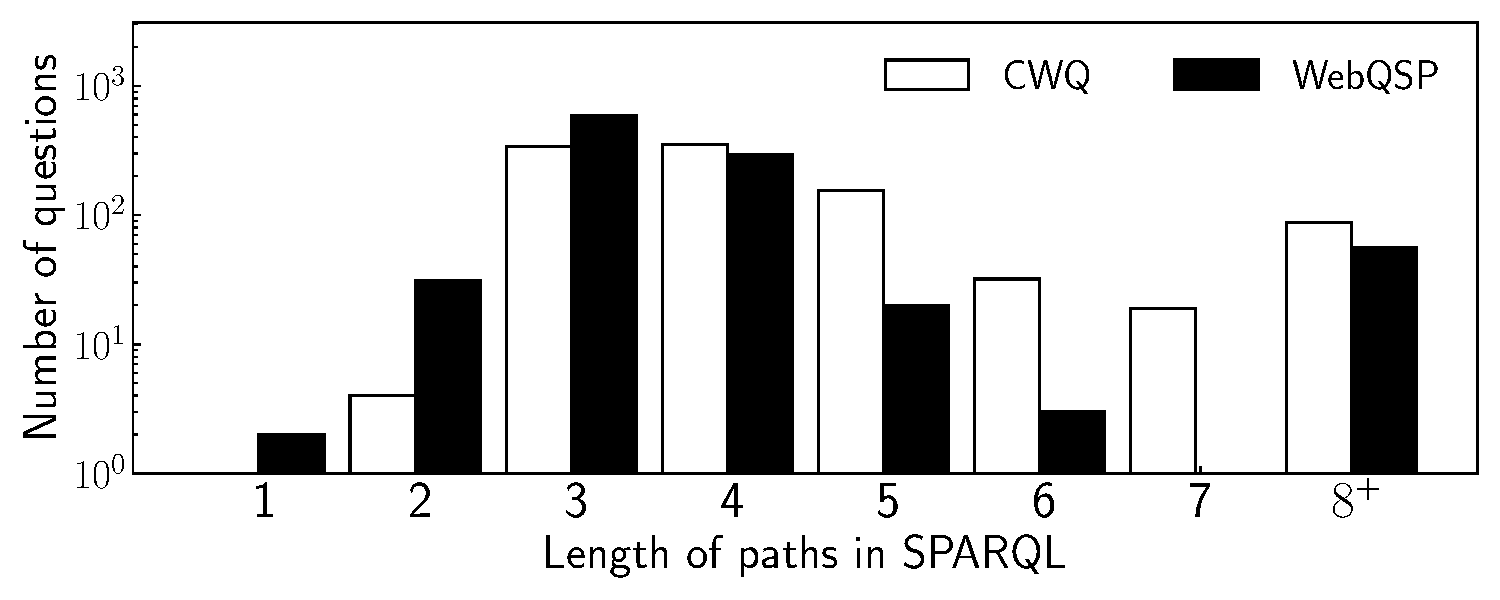
\includegraphics[width=0.9\linewidth]{graphs/Length_of_paths_in_Sparq.pdf}
    \vspace{-2mm}
    \caption{The lengths of the ground-truth SPARQL queries within the CWQ and WebQSP datasets.}
    \vspace{-1mm}
    
    \label{fig:exp:q_by_length}
\end{figure}

\begin{figure}[t]
    % \centering
    \begin{subfigure}{0.48\linewidth}
           \centering
           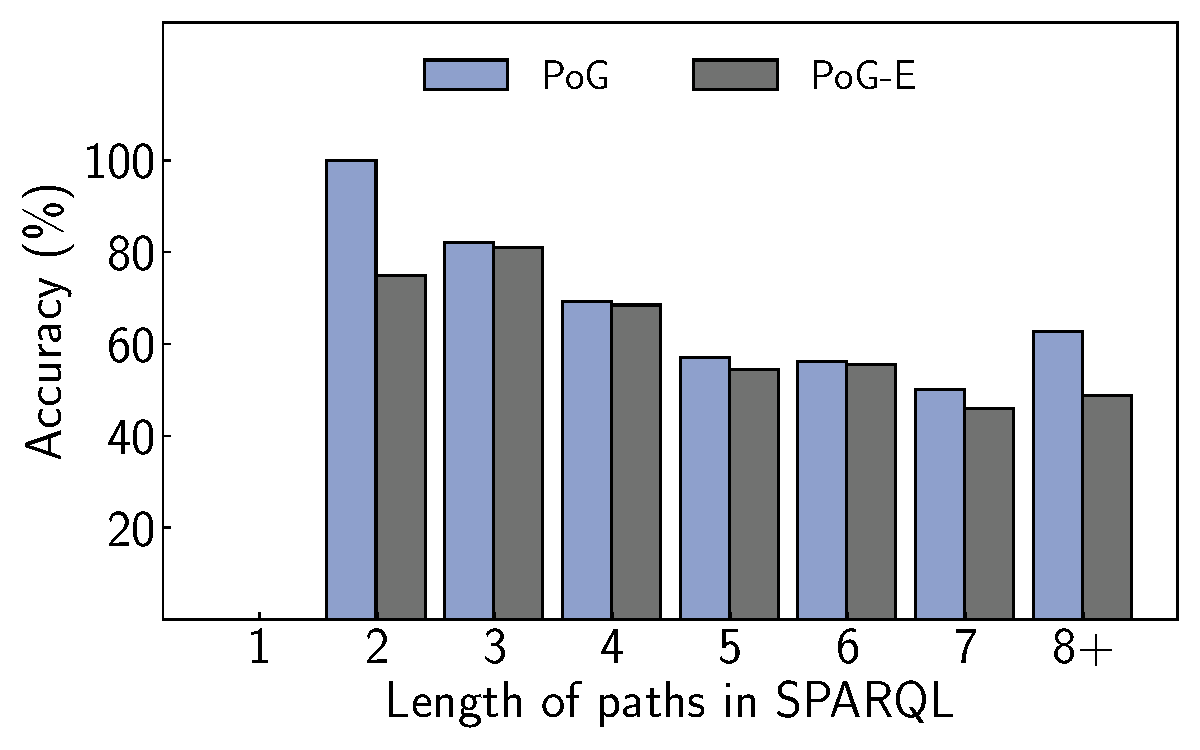
\includegraphics[width=1\linewidth]{graphs/ac_by_length_cwq.pdf}
           % \vspace{-3mm}
           \caption{CWQ}
            \label{fig:aa}
    \end{subfigure}
    \begin{subfigure}{0.48\linewidth}
           \centering
           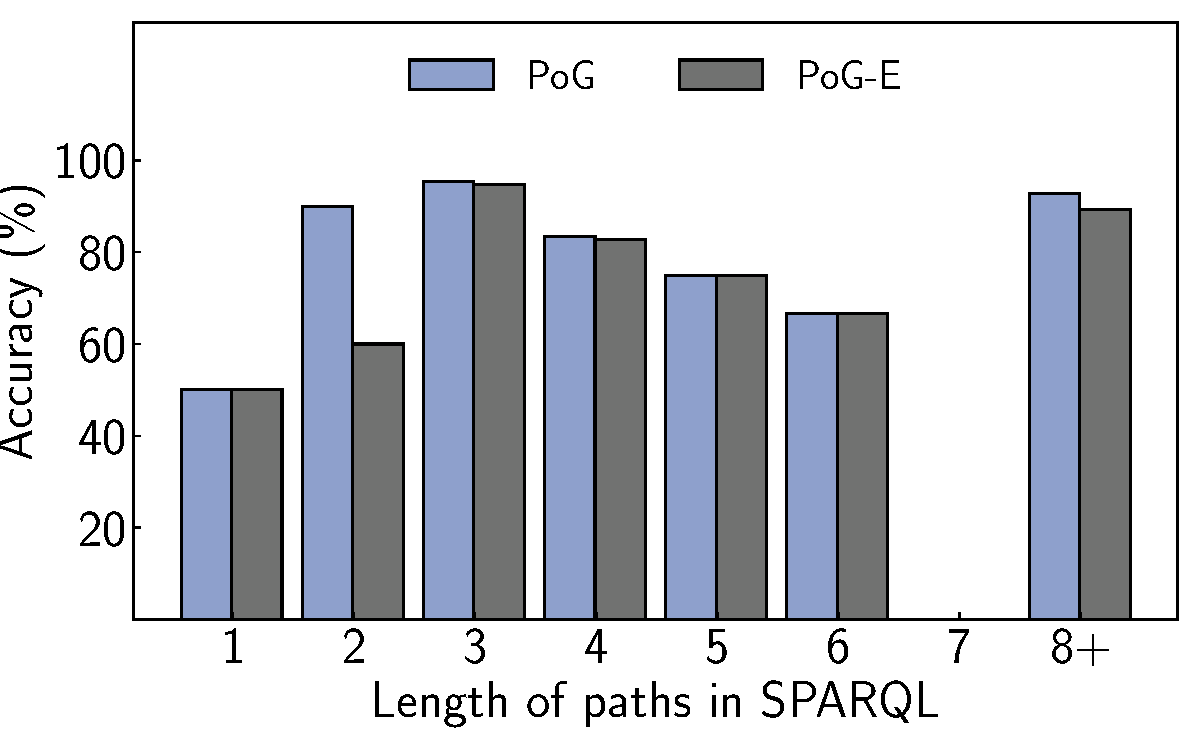
\includegraphics[width=1\linewidth]{graphs/ac_by_length_webqsp.pdf}
           % \vspace{-3mm}
           \caption{WebQSP}
            \label{fig:ab}
    \end{subfigure}
    \vspace{-2mm}
\caption{The accuracy of PoG and PoG-E on the CWQ and WebQSP datasets, categorized by the different lengths of the ground-truth answers for each question.}\label{fig:exp:query_by_length}
    % \vspace{-1mm}
\end{figure}



\myparagraph{Graph structure pruning}
To evaluate the effectiveness of the graph pruning method proposed in Section \ref{method:initialization}, we conduct experiments using 200 random samples from each dataset. We report the average number of entities per question before and after graph reduction, as well as the proportion of entities reduced, in Table \ref{fig:exp:graph_reduction}. The results indicate that up to 54\% of entities in the CWQ dataset can be pruned before path exploration. This demonstrates the effectiveness of eliminating irrelevant data from the outset.
% Please add the following required packages to your document preamble:
% \usepackage{booktabs}
% \vspace{-1mm}

\myparagraph{Case study: interpretable reasoning}
We also conduct the case study to demonstrate interpretability of PoG, we present three reasoning examples in Table \ref{fig:exp:case:interpre} of Appendix \ref{appendix:exp_case_study}. These examples feature questions with one, two, and three entities, respectively. Through the case study, we showcase PoG's effectiveness in handling multi-entity and multi-hop tasks by providing faithful and interpretable reasoning paths that lead to accurate answers.


% \myparagraph{Other Case studies}
To further evaluate the effectiveness and efficiency of PoG, we perform additional experiments, including pruning beam search strategy ablation and prompt setting ablation (Appendix \ref{appendix:Ablation}), reasoning faithfulness analysis (Appendix \ref{appendix:exp:reasoning_faithful}), error analysis (Appendix \ref{appendix:exp:error_analysis}), LLM calls cost and running time analysis (Appendix \ref{appendix:exp:llm_calls}), and graph reduction and path pruning case study (Appendix \ref{appendix:exp_case_study}). 

% These are detailed in Appendix \ref{appendix:expriment}.


% To further assess PoG's effectiveness and efficiency, we perform additional experiments, including prompt setting ablation, reasoning faithfulness analysis, error analysis, LLM cost analysis, and graph reduction case studies. These are detailed in Appendix \ref{appendix:expriment}.

\section{Conclusion}
\label{sec:7_conc}

% In this paper, we introduced Paths-over-Graphs (PoG), a novel method that synergizes LLMs with KGs to achieve faithful and interpretable reasoning. To tackle complex reasoning challenges, PoG employs a three-phase dynamic multi-hop path exploration that integrates the inherent knowledge of LLMs with the factual information from KGs. Efficiency is further enhanced through graph-structured pruning and a three-step pruning process that leverages graph structures, LLM prompting, and pre-trained language models like BERT to effectively narrow down candidate paths. Extensive experiments on five public datasets demonstrate PoG's superior performance, consistently outperforming nearly all in-context and fine-tuning baselines and highlighting its robust reasoning capabilities and interoperability. 


In this paper, we introduce Paths-over-Graphs (PoG), a novel method that integrates LLMs with KGs to enable faithful and interpretable reasoning. PoG addresses complex reasoning tasks through a three-phase dynamic multi-hop path exploration, combining the inherent knowledge of LLMs with factual information from KGs. Efficiency is enhanced by graph-structured pruning and a three-step pruning process to effectively narrow down candidate paths. Extensive experiments on five public datasets demonstrate that PoG outperforms existing baselines, showcasing its superior reasoning capabilities and interoperability. 

\section{Acknowledgment}
Xiaoyang Wang is supported by the Australian Research Council DP230101445 and DP240101322. Wenjie Zhang is supported by the Australian Research Council DP230101445 and FT210100303.





\bibliographystyle{ACM-Reference-Format}
\bibliography{main}

% \renewcommand{\theHsection}{A\arabic{section}}
% \appendixsiam
 

\appendix
% \newpage
% ~

% \newpage
% \section*{Appendix}
% \chapter{Appendix}
\section{Algorithm}

\subsection{Exploration}\label{appendix:alg:explora}
We summarize the comprehensive algorithmic procedure for exploration detailed in Section \ref{method:exploration} as presented in Algorithm \ref{algorithm:explorenreasoning}.

\begin{algorithm}[h]
	{
		{
			\SetVline
			\small
			\caption{{\small{Exploration}}}\label{algorithm:explorenreasoning}
            
			\Input{Question subgraph ($\mathcal{G}_q$), source KG ($\mathcal{G}$),question and split question ($Q = q$ + $q_{split}$), topic entities ($Topic(q)$), LLM indicator ($I_{\text{LLM}}$), predict depth ($D_{\text{predict}}$), maximum depth ($D_{\max}$),  maximum width ($W_{\max}$), and path pruning case ($case$)}
			\Output{PoG answers ($a(q)$), final reasoning path ($Paths_f(q)$)}
            % \State{$T_d^+ \leftarrow$ Obtain positive $k$-truss with smallest query distance $d$ containing $Q$ in Algorithm~\ref{alg_local}}
            % \setstretch{1.25}
            % \tcc{\textcolor{blue}{Start with topic entity path exploration}}
            \vspace{1mm}
            
            \CmtState{\\$List_{T} \leftarrow$ \text{Reorder}($Topic(q), I_{\text{LLM}}$), $D \leftarrow$ min($D_{\text{predict}}, D_{\max}$)} 
            {\textbf{Start with topic entity path exploration}}
            % \State{$D \leftarrow$ min($D_{\text{predict}}, D_{max}$)}
            
            \While{ $D \leq D_{\max}$} {
                \State{$Paths_t \leftarrow \text{EntityPathFind}$ ($List_{T},D$,$\mathcal{G}_q$)}
                \State{$\text{PathPruning}(Paths_t, Q, I_{\text{LLM}}, W_{\max},D_{\max}, List_{T}, case)$}
                \State{$Answer, Paths_{T} \leftarrow \text{QuestionAnswering}(Paths_t, Q, I_{\text{LLM}})$}

                
                \State{\textbf{if}  $\texttt{"\{Yes\}"} \text{ in } Answer$  \textbf{then} \textbf{return} $Answer, Paths_{T}$;\\ \textbf{else} $D \leftarrow D + 1$}
			}
    % \State{\textbf{if} $Answer$ = True \textbf{then} \textbf{return} $Answer, Paths_{T}$ }

% \textcolor{blue}{\tcc{LLM supplement path exploration procedure}}
\vspace{1mm}
\CmtState{\\$Paths_s \leftarrow []$}{\textbf{LLM supplement path exploration procedure} }

\State{$ Predict(q) \leftarrow  $SupplementPrediction($Paths_T, Q, I_{\text{LLM}}$)} 
\ForEach{ $e,I_{sup(e)} \in Predict(q)$} {
    % \State{$List_{S} \leftarrow $ $List_{T} +e$ }
    
    \State{$List_{S} \leftarrow $ Reorder ($List_{T} +e, I_{sup(e)}$)}
    \State{$Paths_s' \leftarrow \text{EntityPathFind}$ ($List_{S},D_{\max}$,$\mathcal{G}_q$)}
    \State{$Paths_s \leftarrow  Paths_s + \text{FuzzySelect}$ ($Paths_s', I_{sup(e)}, W_{\max}$)}
    }

    \State{$ \text{PathPruning}(Paths_s, Q, I_{\text{LLM}}, W_{\max},D_{\max}, List_{S}, case)$}
    \State{$Answer, Paths_{S} \leftarrow \text{QuestionAnswering}(Paths_s, Q, I_{\text{LLM}})$}

    % \State{$Answer, Paths_{S} \leftarrow \text{Reasoning}(Paths_s, Q, I_{\text{LLM}})$}
   
   


    \State{\textbf{if} \texttt{"\{Yes\}"} in $Answer$ \textbf{then} \textbf{return} $Answer, Paths_{S}$ }
    

% \textcolor{blue}{\tcc{Node expand exploration procedure}}
\vspace{1mm}

   \CmtState{\\$Visted \leftarrow \emptyset$, $D\leftarrow1$, $Paths_e \leftarrow Paths_{T} +Paths_{S} $}{\textbf{Node expand exploration procedure} }
   % \State{$Paths_e \leftarrow Paths_{T} +Paths_{S} $}
   % \If{$|Paths_e| > W_{max}$} {
   % $\text{PathsPruning}(Paths_e, Q, I_{\text{LLM}}, W_{max}, D_{max}, List_{T}, case)$;}
   \State{$\text{PathPruning}(Paths_e, Q, I_{\text{LLM}}, W_{\max}, D_{\max}, List_{T}, case)$;}

   \While{$D\leq D_{\max}$} {
    % \State{$Entities \leftarrow$ ExtractEntity($Paths_e$)}
    \ForEach{$e \in \text{ExtractEntity}(Paths_e) \land e \notin Visted$} {
        \State{$Related\_edges = \text{Find\_1\_hop\_Edges}(\mathcal{G}, e)$}
        \State{$Paths_e \leftarrow \text{MergeTogether}(Paths_e, Related\_edge)$}

        
        % \State{$Visted = Visted \cup e$; $D\leftarrow D+1$}
    }
    \State{$\text{PathPruning}(Paths_e, Q, I_{\text{LLM}}, W_{\max},D_{\max},List_{T}, case)$}
    \State{$Answer, Paths_{e} \leftarrow \text{QuestionAnswering}(Paths_e, Q, I_{\text{LLM}})$}
    % \State{\textbf{if} $Answer$ = True \textbf{then} \textbf{return} $Answer, Paths_{e}$ }
    \State{\textbf{if} $ \texttt{"\{Yes\}"} \text{ in } Answer$  \textbf{then} \textbf{return} $Answer, Paths_{e}$;\\ \textbf{else} $Visted \leftarrow Visted \cup e$; $D\leftarrow D+1$}
}

    \State{
    $Paths_l \leftarrow Paths_T+Paths_S+Paths_E$
    }
    \State{
    $ \text{PathPruning}(Paths_l, Q, I_{\text{LLM}}, W_{\max},D_{\max}, List_{T},case)$}
    
    \State{$Answer,Paths_L \leftarrow \text{QuestionAnsweringFinal}(Paths_l, Q, I_{\text{LLM}})$}
    \State{\textbf{Return} $Answer,Paths_L$}
    % \textbf{Procedure} PathsReasoning$(Paths_{t}, Q, I)$\\
    % \SetVline
    % \small
    % % \If{$v \neq Q$}{
    % \StateCmt{$Paths_{f} \leftarrow \text{PathPathsPruning} (Paths_{t}, Q,  I)$}{Utilizing Bi}
    
    
    % \State{$Answer, Paths_{f} \leftarrow \text{QA}(Paths_{f}, Q,  I_{\text{LLM}})$}
}
}
\end{algorithm}
\newpage
\subsection{Path Pruning}\label{appendix:alg:pathpruning}
We summarize the comprehensive algorithmic procedure of path pruning detailed in Section \ref{method:3pathprune} as presented in Algorithm \ref{algorithm:PathsPruning}. 

\begin{algorithm}[h]
	{
		{
			\SetVline
			\small
			\caption{{\small{PathPruning}}}\label{algorithm:PathsPruning}
            
			\Input{Candidate paths($Paths_{c}$), question and split question ($Q = q+ q_{split}$), indicator ($I$), maximum width ($W_{\max}$), maximum depth ($D_{\max}$), entity list ($list$)}
			\Output{Pruned candidate paths ($Paths_{c}$)}
            % \State{$T_d^+ \leftarrow$ Obtain positive $k$-truss with smallest query distance $d$ containing $Q$ in Algorithm~\ref{alg_local}}
            % \setstretch{1.25}
            % \tcc{\textcolor{blue}{Start with topic entity path exploration}}
            \If{Case = \texttt{Fuzzy Selection Only}}
            {
            \State{$ \text{FuzzySelect}(Paths_{c},Q, I,W_{\max})$}}
            \ElseIf{Case = \texttt{Fuzzy + Precise Path Selection}}
            {
            \State{$ \text{FuzzySelect}(Paths_{c},Q, I,W_{1})$}
            \State{$ \text{PrecisePathSelect}(Paths_{c},Q, I,W_{\max})$}
            } 
            \ElseIf{Case = \texttt{Fuzzy + Branch Reduced Selection}}
            {
            \State{$ \text{FuzzySelect}(Paths_{c},Q, I,W_{1})$}
            \State{$ \text{BranchReduceSelect}(Paths_{c},Q, I,W_{\max},D_{\max},list)$}
            
            }
            \ElseIf{Case = \texttt{Fuzzy + Branch Reduced + Precise Path}}
            {
            \CmtState{$ \text{FuzzySelect}(Paths_{c},Q, I,W_{1})$} 
            {case = 3-Step Beam Search}
            \State{$ \text{BranchReduceSelect}(Paths_{c},Q, I,W_{2},D_{\max},list)$}
            \State{$ \text{PrecisePathSelect}(Paths_{c},Q, I,W_{\max})$}
            
            }
        % \State{\textbf{Return} $Paths_{c}$}
            \vspace{1mm}
            \textbf{Procedure} BranchReduceSelect$(Paths_{c}, Q, I, W, D_{\max}, list)$\\
            \SetVline
            \small
            % \If{$v \neq Q$}{
            \State{$D \leftarrow 1$, $Paths_{e} \leftarrow \emptyset$}
            % \State{}
            
            \While{$|Paths_{c}| \geq W \land D \leq D_{\max}$} {

                
            \ForEach{$e\in list$} {
                
                \State{$Paths_{e} \leftarrow Paths_{e} \cup \text{ExtractHeadSteps}(Paths_{c}, e, D)$}
            }
            \If{$|Paths_{e}| > W$} {
                \State{$ \text{PrecisePathSelect}(Paths_{e},Q, I,W)$}
            
                \State{$Paths_{c} \leftarrow \text{IntersectMatchUpdate}(Paths_{e}, Paths_{c})$}
                \State{$Paths_{e} \leftarrow \emptyset$}
            }
            \State{$D\leftarrow D+1$}
        }

            \State{\textbf{if} $|Paths_{c}| > W$ \textbf{then} $ \text{PrecisePathSelect}(Paths_{c},Q, I,W)$}

    }
    }
\end{algorithm}




\newpage
\section{Experiment}\label{appendix:expriment}

\subsection{Additional Ablation Study}\label{appendix:Ablation}


\myparagraph{Compare the effect of different beam search strategies} As introduced in Section \ref{method:3pathprune}, PoG supports various beam search strategies, ranging from non-reliant to fully reliant on LLMs, selectable in a user-friendly manner. To evaluate the computational cost and performance, we test four cases outlined in Algorithm \ref{algorithm:PathsPruning}. In the \texttt{3-Step Beam Search} case, we set $W_2 = 20$ for internal narrowing. The \texttt{Fuzzy Selection} approach, as described in Section \ref{method:3pathprune}, utilizes all candidate paths and a LLM-generated indicator for encoding and comparison.
% We measure accuracy, average LLM calls, and average token input to the LLM API during the path pruning phase to measure efficiency and effectiveness
% We report accuracy, average LLM calls, and average token input during the path pruning phase for each beam search strategy in Table \ref{fig:ablation:vary_beamsearch} for PoG. 
% The experiment result of PoG-E is detailed in Table \ref{fig:ablation:vary_beamsearch_pog-e} of Appendix \ref{appendix:Ablation}. 
We report accuracy, average LLM calls in total, and average token input during the path pruning for each beam search strategy applied to PoG and PoG-E in Table \ref{fig:ablation:vary_beamsearch} and Table \ref{fig:ablation:vary_beamsearch_pog-e}.
These results indicate that PoG/PoG-E with \texttt{Fuzzy and Precise Path Selection} achieves the highest accuracy. Additionally, the \texttt{BranchReduced Selection} method, which leverages the graph structure, not only delivers excellent results but also reduces token usage by over 50\% (65\%) with only a ±2\% (±4.3\%) difference in accuracy on PoG (PoG-E) compared to the best-performing strategy. Furthermore, the \texttt{Fuzzy Selection} method, which employs lightweight models instead of relying solely on LLMs, also demonstrates strong performance. These results validate the effectiveness of our beam search strategies and underscore the importance of structure-based faithful path reasoning. 
% The performance result of PoG-E is shown in Table \ref{fig:ablation:vary_beamsearch_pog-e}.
% Please add the following required packages to your document preamble:
% \usepackage{booktabs}
% \usepackage[normalem]{ulem}
% \useunder{\uline}{\ul}{}


\begin{table}[h]
\caption{Performance comparison of PoG with different beam search methods on CWQ and WebQSP.}\label{fig:ablation:vary_beamsearch}
\begin{tabular}{@{}llcc@{}}
% \small
\toprule
\textbf{PoG}              & \textbf{Evaluation} & \textbf{CWQ}  & \textbf{WebQSP} \\ \midrule
w/ Fuzzy Selection        & Accuracy           & 57.1          & 86.4           \\
                          & Token Input         & -             & -               \\
                          & LLM Calls       & 6.8           & 6.5             \\ \midrule
w/ Fuzzy and              & Accuracy           & 79.3          & {\ul 93.0}     \\
BranchReduced Selection & Token Input         & 101,455       & 328,742         \\
                          & LLM Calls       & 9.7         & 9.3             \\ \midrule
w/ Fuzzy and              & Accuracy           & \textbf{81.4} & \textbf{93.9}   \\
Precise Path Selection    & Token Input         & 216,884       & 617,448         \\
                          & LLM Calls       & 9.1           & 7.5             \\ \midrule
w/ 3-Step Beam Search    & Accuracy           & {\ul 79.8}    & 91.9            \\
                          & Token Input         & 102,036       & 369,175         \\
                          & LLM Calls       & 8.8           & 9.0               \\ \bottomrule
\end{tabular}
\end{table}

\newpage
\myparagraphquestion{How do summary prompts affect} 
Inspired by GoT \cite{besta2024graphGoT}, we utilize summary prompts to reduce LLM hallucinations and decrease computational costs. To evaluate their impact, we conduct an ablation study comparing PoG and PoG-E with and without path summarization. We measure both accuracy and average token input to the LLM API during the path pruning phase to measure efficiency and effectiveness.
The results, present in Tabel \ref{fig:ablation:summ_prompt}, show that using graph summaries increases accuracy by up to 10\% on the CWQ dataset with PoG-E, while reducing token input by up to 36\% on WebQSP. These results indicate hat path summarization effectively minimizes LLM hallucinations, enhances the LLM's understanding of the explored paths, facilitates answer retrieval, enables earlier termination of the reasoning process, and reduces costs.
\begin{table}[h]

\caption{Performance comparison of PoG-E with different beam search methods among CWQ and WebQSP datasets.}\label{fig:ablation:vary_beamsearch_pog-e}
\begin{tabular}{@{}llcc@{}}
\toprule
\textbf{PoG-E}          & \textbf{Evaluation} & \textbf{CWQ}  & \textbf{WebQSP} \\ \midrule
w/ FuzzySelect          & Accuracy           & 62.31         & 82.3            \\
                        & Token Input         & -             & -               \\
                        & Ave LLM Calls       & 6             & 6.3             \\ \midrule
w/ Fuzzy and            & Accuracy           & 71.9          & 88.4            \\
BranchReduced Selection & Token Input         & 128,407       & 371,083         \\
                        & Ave LLM Calls       & 9.4           & 9.1             \\ \midrule
w/ Fuzzy and            & Accuracy           & \textbf{80.4} & \textbf{91.4}   \\
Precise Path Selection  & Token Input         & 344,747       & 603,261         \\
                        & Ave LLM Calls       & 8.3           & 7.4             \\ \midrule
w/ 3-Step Beam Search  & Accuracy           & {\ul 73.87}   & {\ul 89.4}      \\
                        & Token Input         & 120,159       & 411,283         \\
                        & Ave LLM Calls       & 8.3           & 9.1             \\ \bottomrule
\end{tabular}

\end{table}

\begin{table}[h]
\caption{Performance comparison of PoG and PoG-E with and without path summarizing on CWQ and WebQSP datasets.}\label{fig:ablation:summ_prompt}
\begin{tabular}{@{}llcc@{}}
\toprule
\textbf{Method}      & \textbf{Evaluation} & \textbf{CWQ} & \textbf{WebQSP} \\ \midrule
\textbf{PoG}         &                     &              &                 \\
w/ Path Summarizing   & Accuracy           & \textbf{81.4 }        & \textbf{93.9}            \\
                     & Token Input         & 216,884      & 297,359         \\
w/o Path Summarizing & Accuracy           & 74.7         & 91.9            \\
                     & Token Input         & 273,447      & 458,545         \\ \midrule
\textbf{PoG-E}       & \textbf{}           & \textbf{}    & \textbf{}       \\
w/ Path Summarizing   & Accuracy           & \textbf{80.4 }        & \textbf{91.4}            \\
                     & Token Input         & 314,747      & 273,407         \\
w/o Path Summarizing & Accuracy           & 70.4         & 90.4            \\
                     & Token Input         & 419,679      & 428,545         \\ \bottomrule
\end{tabular}
\end{table}
% Please add the following required packages to your document preamble:
% \usepackage{booktabs}


% Please add the following required packages to your document preamble:
% \usepackage{booktabs}
% \usepackage[normalem]{ulem}
% \useunder{\uline}{\ul}{}

\newpage
\subsection{Reasoning Faithfulness Analysis}\label{appendix:exp:reasoning_faithful}
\myparagraph{Overlap ratio between explored paths and ground-truth paths}
We analyzed correctly answered samples from three datasets to investigate the overlap ratio between the paths $P$ explored by PoG and the ground-truth paths $S$ in SPARQL queries. The overlap ratio is defined as the proportion of overlapping relations to the total number of relations in the ground-truth SPARQL path:

\[
Ratio(P) = \frac{|Relation(P) \cap Relation(S)|}{|Relation(S)|},
\]

\noindent where $Relation(P)$ denotes the set of relations in path $P$.
Figure \ref{fig:exp:overlap} illustrates the distribution of questions across different overlap ratios. For the WebQSP dataset, PoG achieves the highest proportion of fully overlapping paths with the ground truth, reaching approximately 60\% accuracy. In contrast, PoG-E applied to the GrailQA dataset shows the highest proportion of paths with up to 70\% non-overlapping relations, indicating that PoG-E explores novel paths to derive the answers.
The different results between PoG and PoG-E are due to PoG-E's strategy of randomly selecting one related edge from each clustered edge. This approach highlights the effectiveness of our structure-based path exploration method in generating diverse and accurate reasoning paths.


\begin{figure}[h]
    % \centering
    \begin{subfigure}{0.495\linewidth}
           \centering
           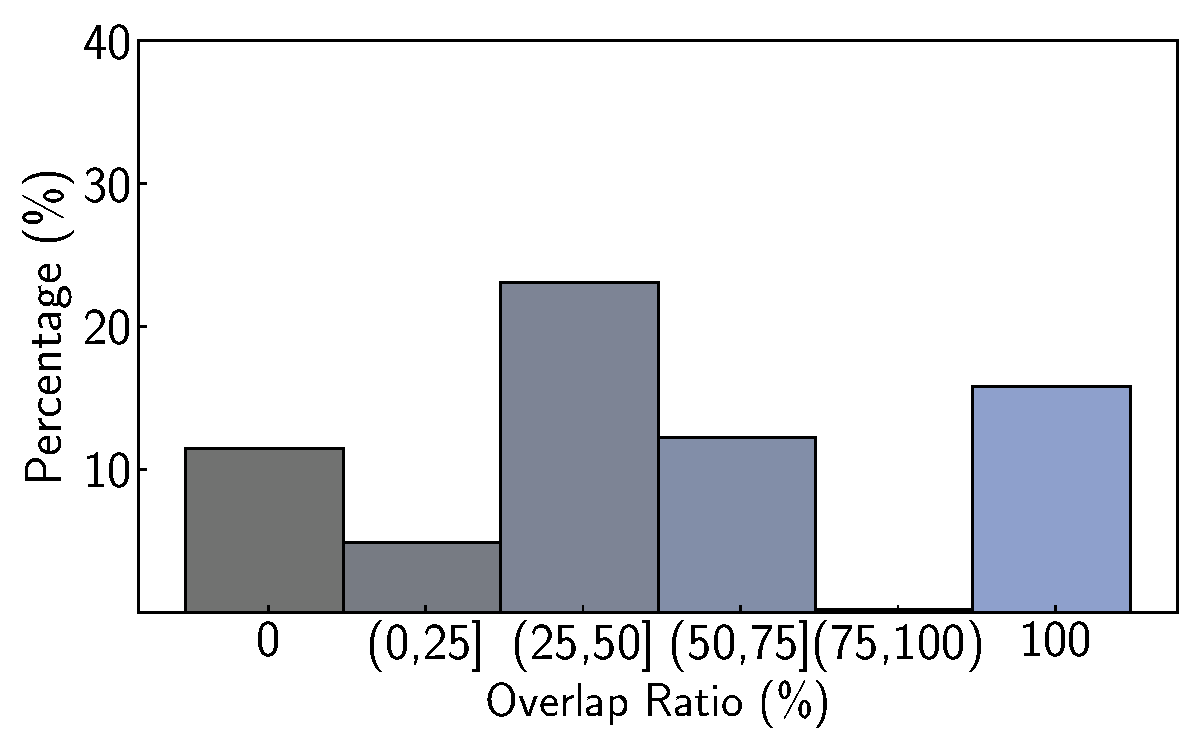
\includegraphics[width=1\linewidth]{graphs/path_overlap_cwq_pog_1.pdf}
           
           \caption{CWQ (PoG)}
            \label{fig:a}
    \end{subfigure}
    \begin{subfigure}{0.495\linewidth}
           \centering
           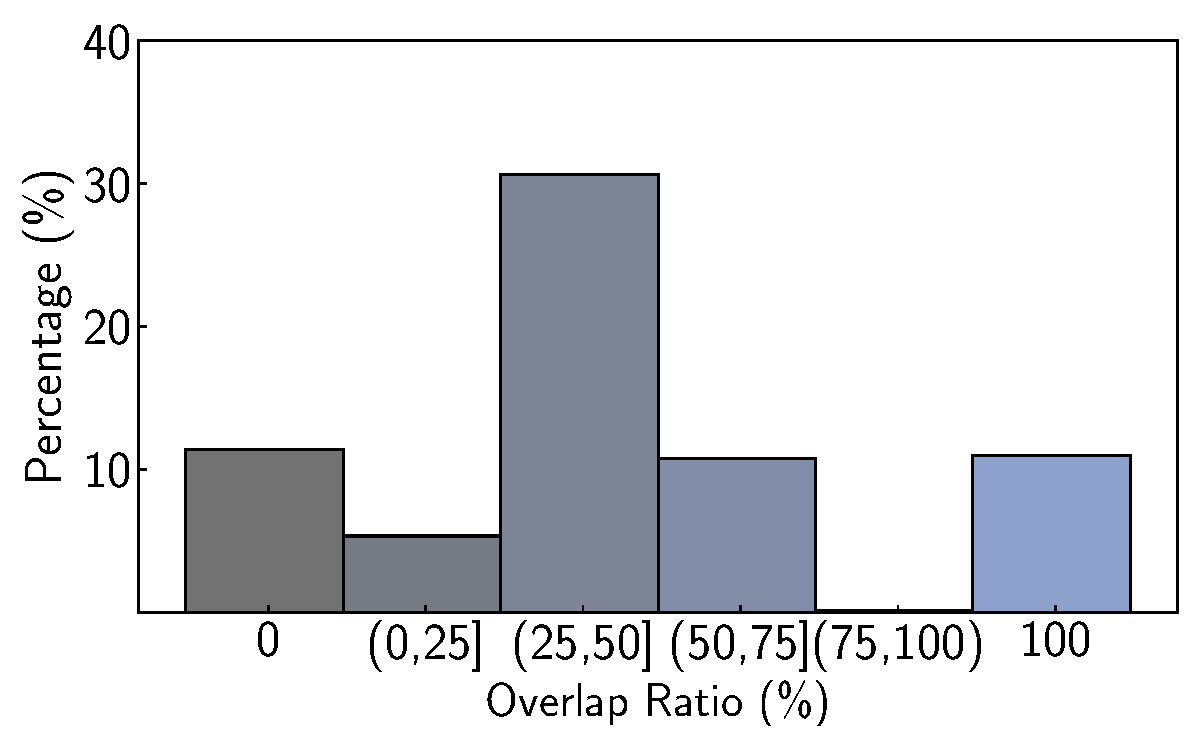
\includegraphics[width=1\linewidth]{graphs/path_overlap_cwq_pog_e.pdf}
           
           \caption{CWQ (PoG-E)}
            \label{fig:a}
    \end{subfigure}
    \begin{subfigure}{0.495\linewidth}
           \centering
           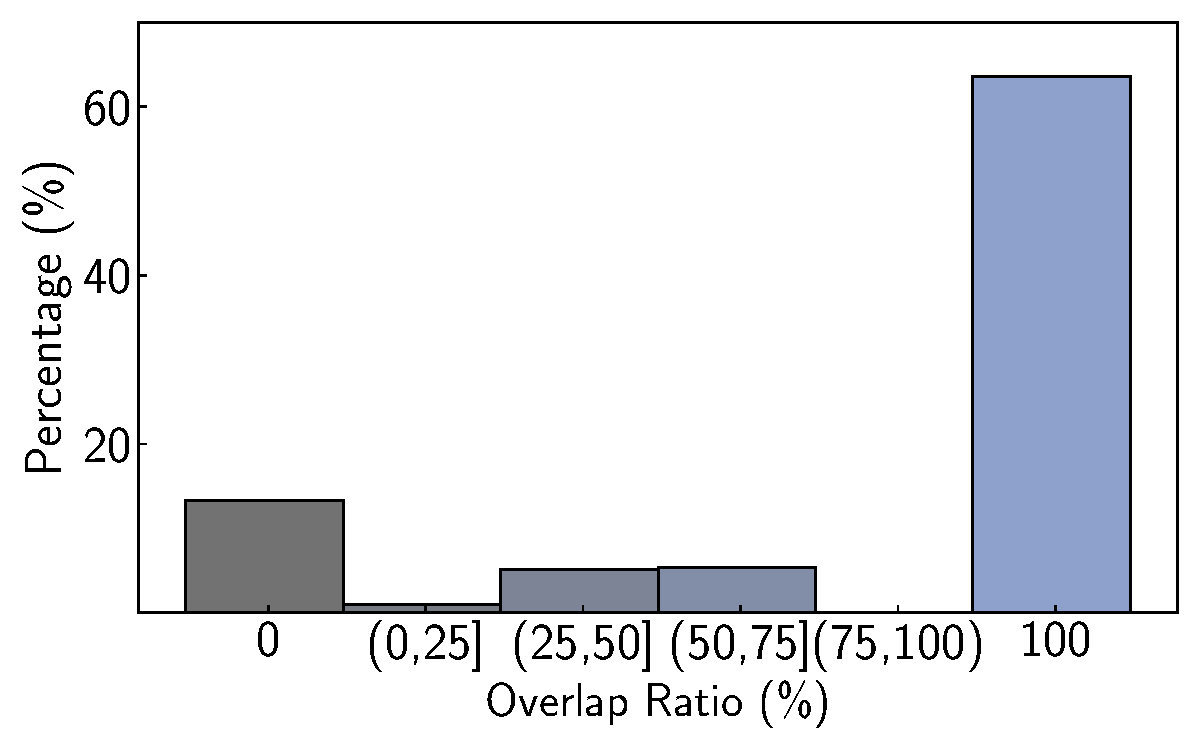
\includegraphics[width=1\linewidth]{graphs/path_overlap_webqsp_pog_1.pdf}
           
           \caption{WebQSP (PoG)}
            \label{fig:a}
    \end{subfigure}
    \begin{subfigure}{0.495\linewidth}
           \centering
           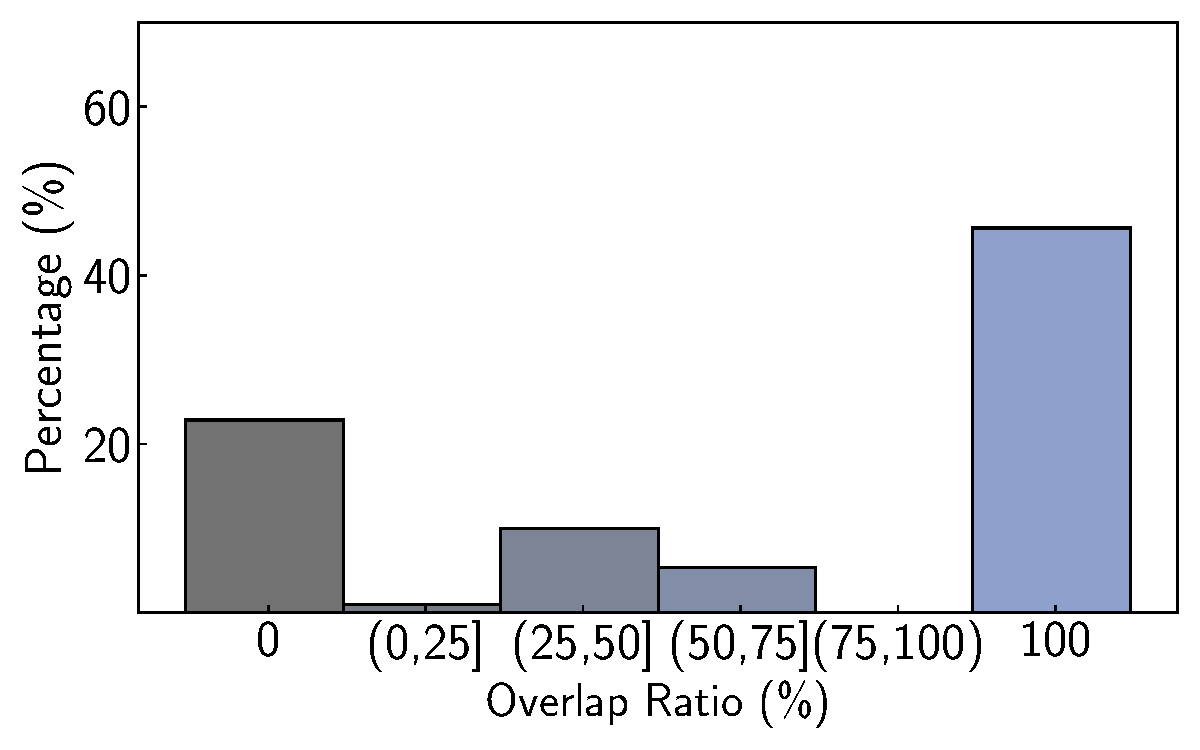
\includegraphics[width=1\linewidth]{graphs/path_overlap_webqsp_pog_e.pdf}
           
           \caption{WebQSP (PoG-E)}
            \label{fig:a}
    \end{subfigure}
    \begin{subfigure}{0.495\linewidth}
           \centering
           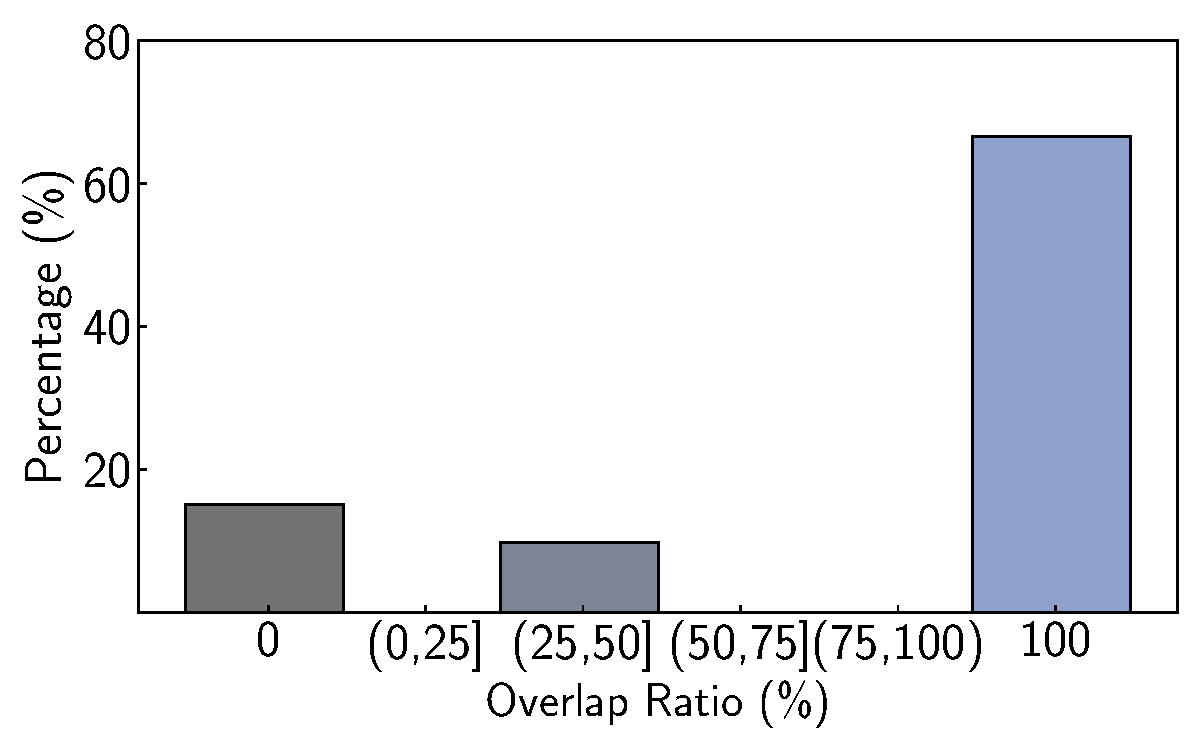
\includegraphics[width=1\linewidth]{graphs/path_overlap_grailqa_pog_1.pdf}
           
           \caption{GrailQA (PoG)}
            \label{fig:a}
    \end{subfigure}
    \begin{subfigure}{0.495\linewidth}
           \centering
           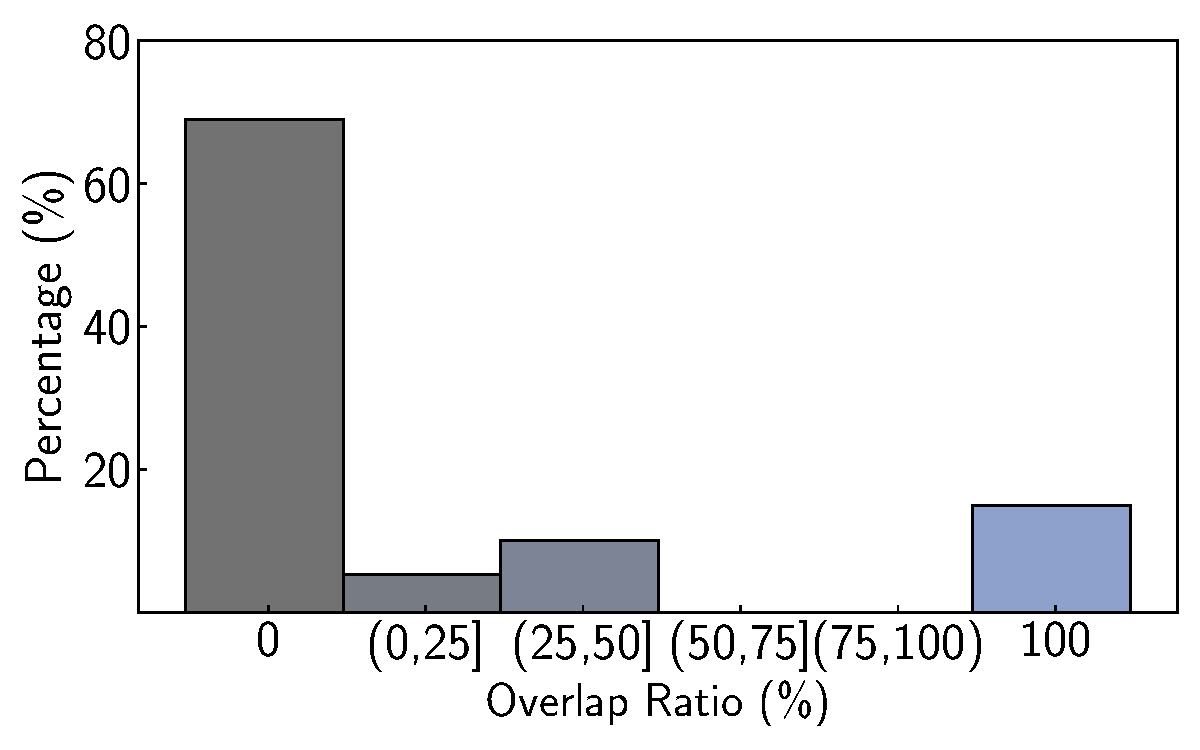
\includegraphics[width=1\linewidth]{graphs/path_overlap_grailqa_pog_e.pdf}
           
           \caption{GrailQA (PoG-E)}
            \label{fig:a}
    \end{subfigure}
    
\caption{ The path overlap ratio of PoG and PoG-E among CWQ, WebQSP, and GrailQA datasets.}\label{fig:exp:overlap}
    
\end{figure}

\newpage
\myparagraph{Evidence of answer exploration sources}
We conduct an analysis of correctly answered samples from three datasets to investigate the sources of evidence used by the LLM in generating answers, as illustrated in Figure \ref{fig:exp:answer_gen_by}. Specifically, we categorize all generated answers into three cases: KG only, LLM-inspired KG, and KG-inspired LLM.
In the \textit{KG only} scenario, answers are generated solely based on KG paths. The \textit{LLM-inspired KG} case involves the LLM predicting an answer using its inherent knowledge and subsequently using the KG to verify its correctness. Conversely, in the \textit{KG-inspired LLM} case, the paths generated by the KG are insufficient to reach the answer, and the LLM supplements the reasoning using its inherent knowledge.
As shown in the figure, up to 14\% of answers are generated through the KG-inspired LLM approach, and up to 9\% involve LLM-inspired KG path supplementation. Compared to previous work that integrates LLM inherent knowledge with KG data\cite{tog1.0sun2023think}, PoG more effectively leverages the strengths of both sources. These results demonstrate that PoG is a faithful reasoning method that primarily relies on KG-based reasoning while being supplemented by the LLM, ensuring both accuracy and interpretability in answer generation.
\begin{figure}[h]
    % \centering
    % 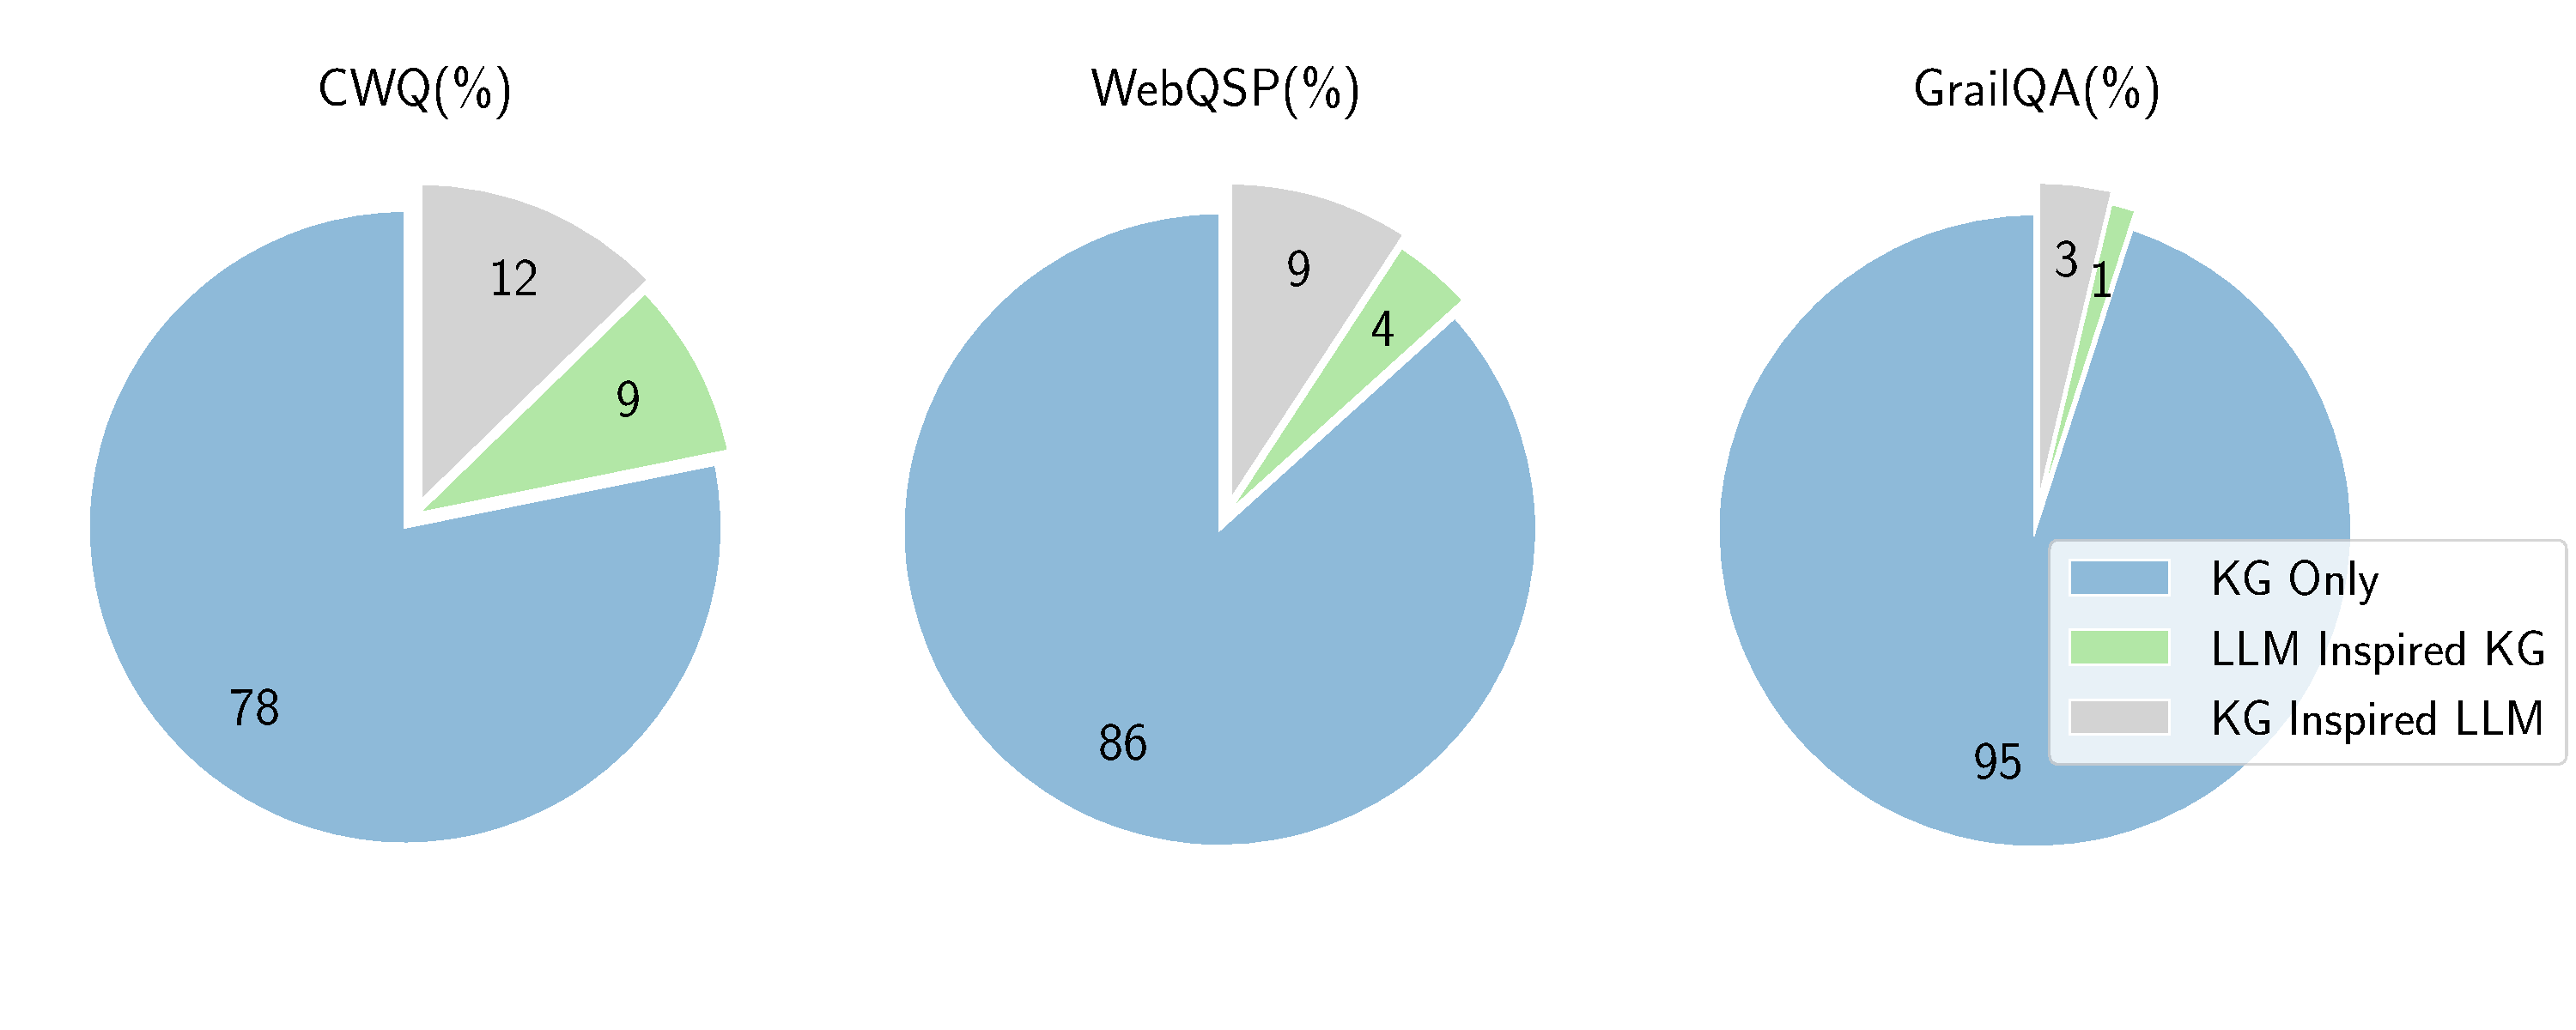
\includegraphics[width=0.34\linewidth]{graphs/answer_precentage_PoG.pdf}
    % \vspace{-5mm}
    % \caption{The lengths of the ground-truth Sparql queries within the CWQ and WebQSP datasets.}
    % \label{fig:enter-label}
    % \centering
    \begin{subfigure}{1\linewidth}
           \centering
           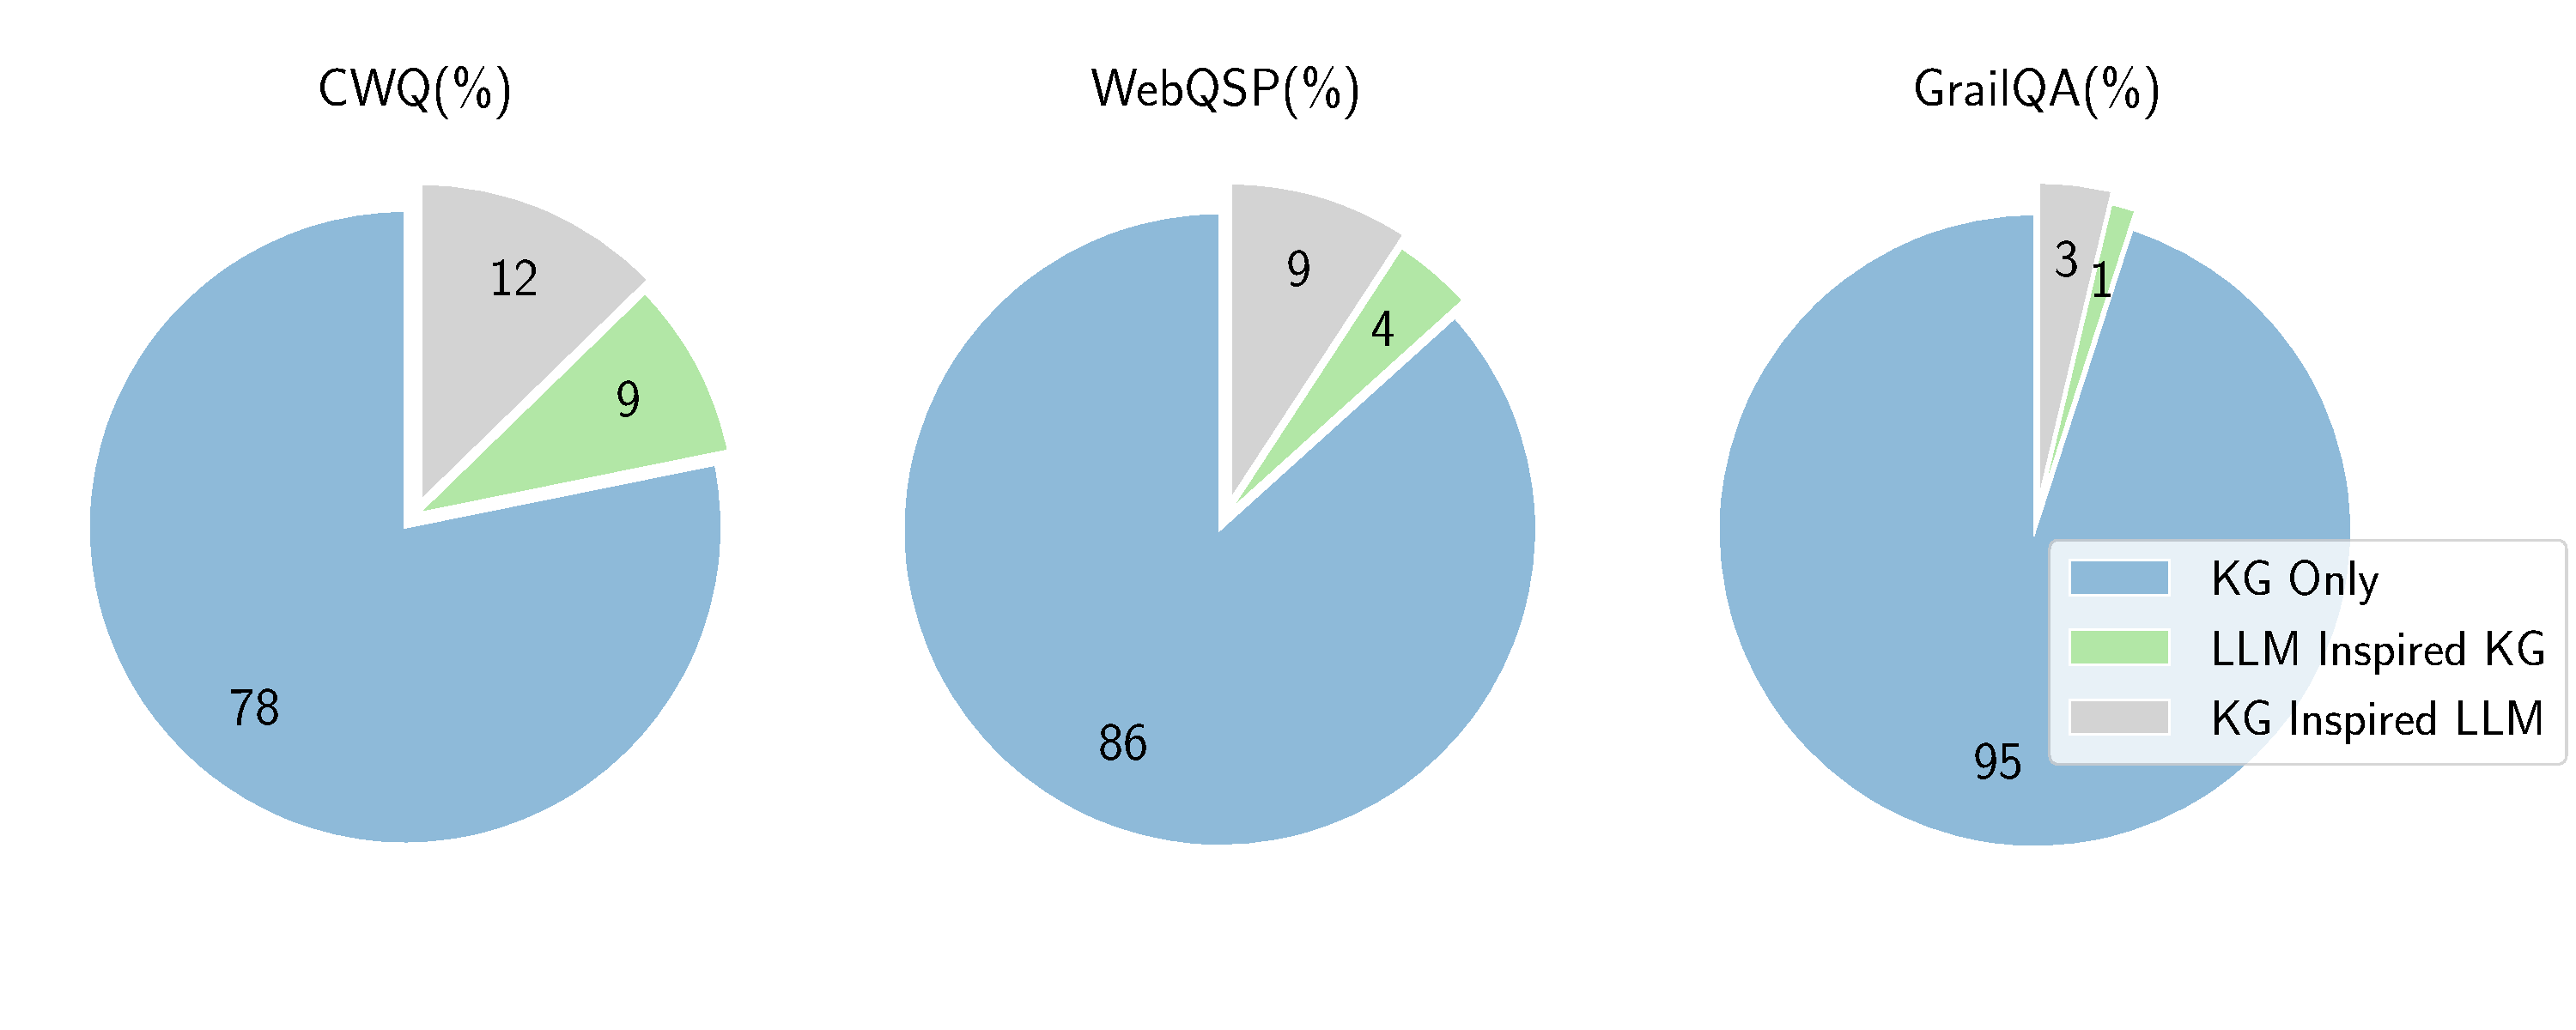
\includegraphics[width=1\linewidth]{graphs/answer_precentage_PoG.pdf}
           
           \caption{PoG}
            \label{fig:a}
    \end{subfigure}
    \begin{subfigure}{0.99\linewidth}
           \centering
           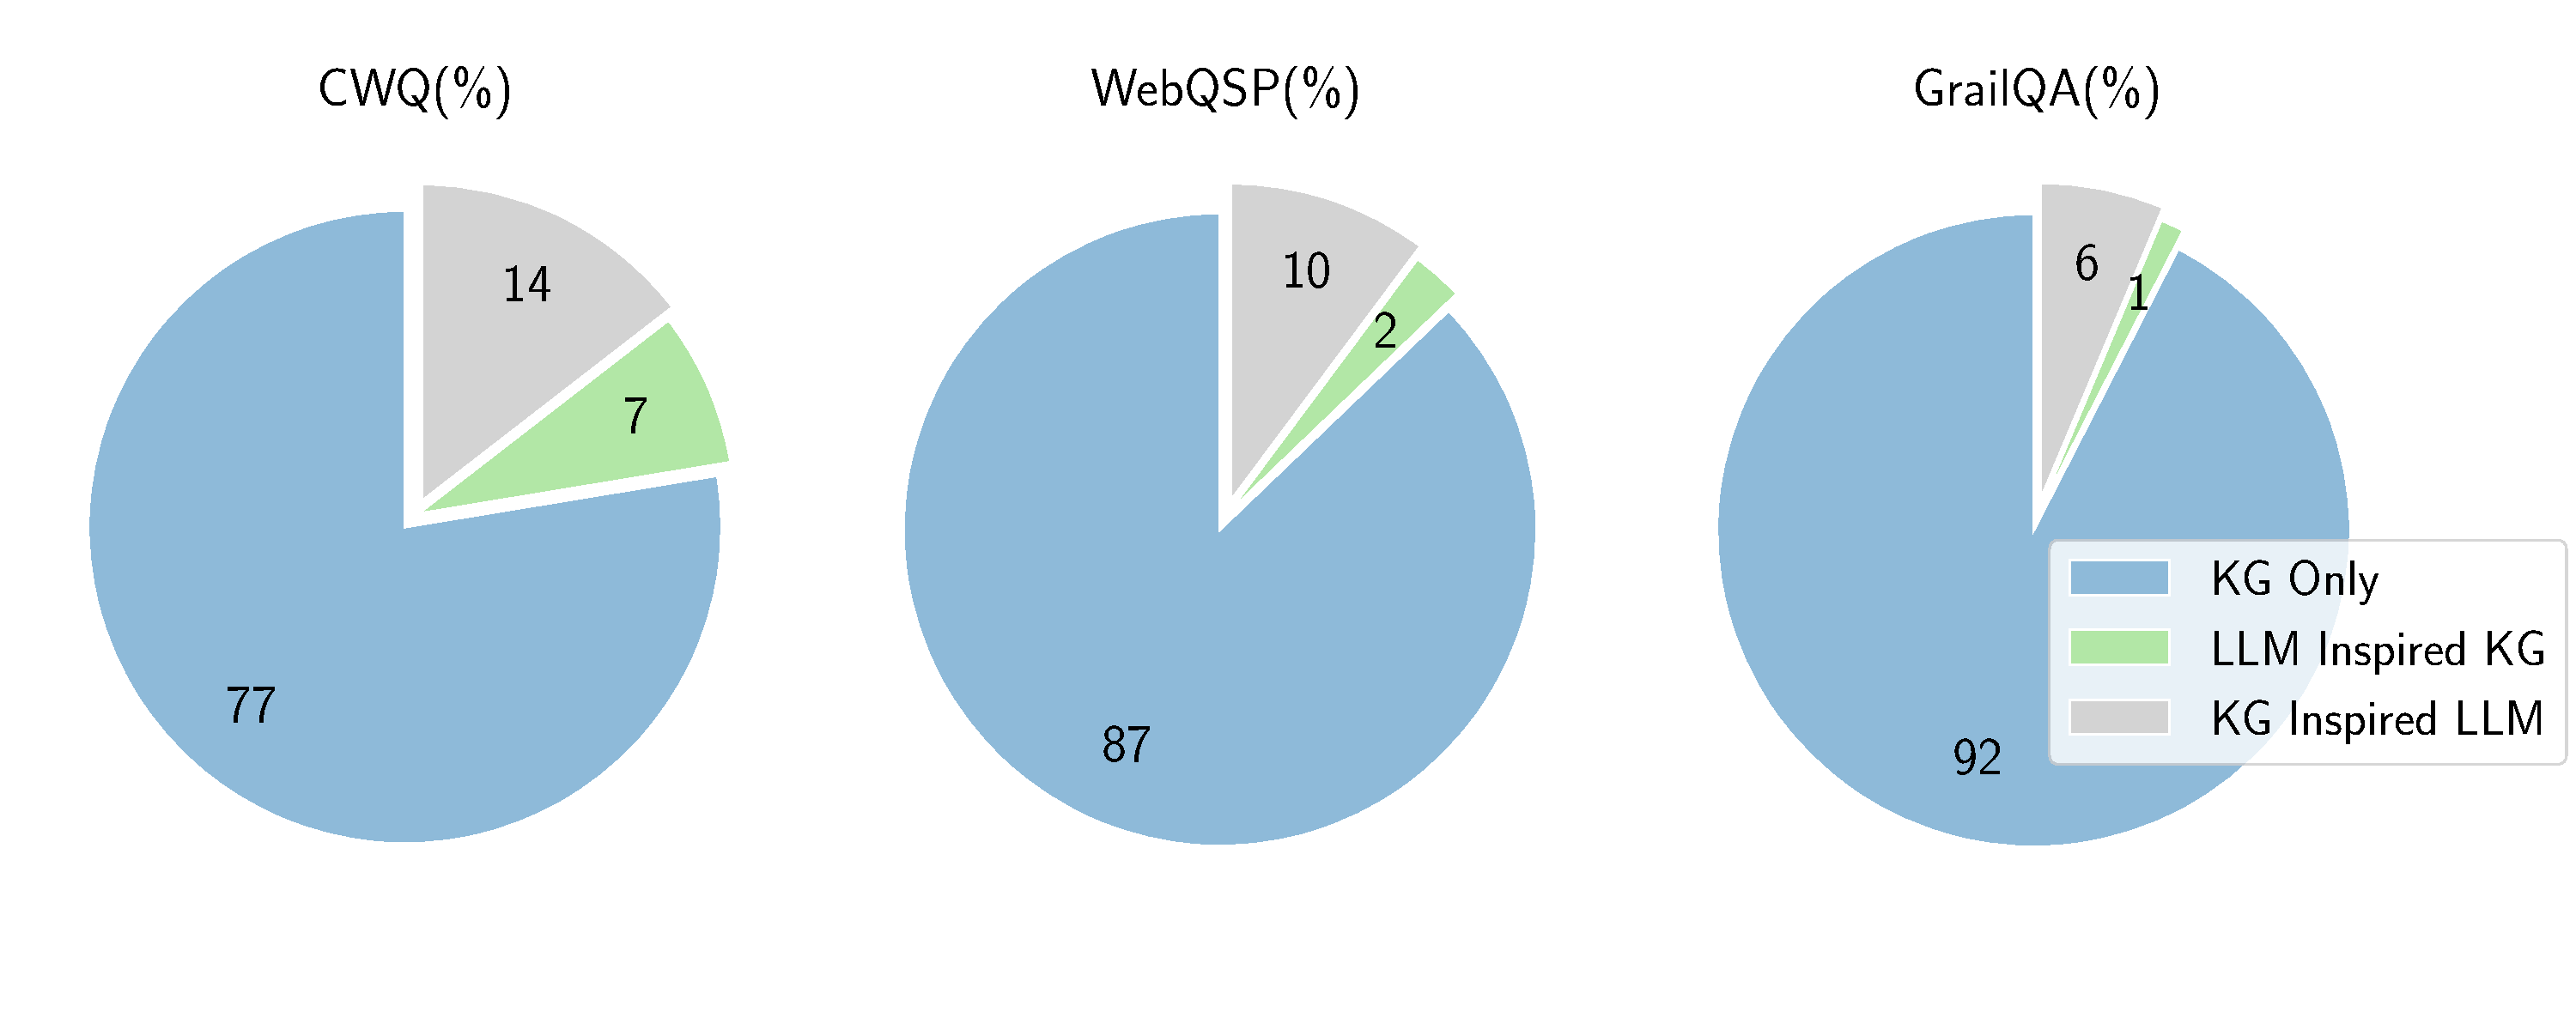
\includegraphics[width=1\linewidth]{graphs/answer_precentage_PoG_e.pdf}
           
           \caption{PoG-E}
            \label{fig:a}
    \end{subfigure}
    
\caption{The proportions of answer evidence of PoG and PoG-E among CWQ, WebQSP, and GrailQA datasets.}\label{fig:exp:answer_gen_by}
\end{figure}




\newpage
\subsection{Error Analysis}\label{appendix:exp:error_analysis}

% \myparagraph{Error analysis}
To further analyze the integration of LLMs and KGs, we conduct an error analysis on the CWQ, WebQSP, and GrailQA datasets. We categoriz errors into four types: (1) answer generation error, (2) refuse error, (3) format error, and (4) other hallucination errors. Note that answer generation error occurs when PoG provides an accurate reasoning path, but the LLM fails to extract the correct answer from it.
The distribution of these error types is illustrated in Figure \ref{fig:exp:error_analysis}. The results indicate that using more powerful LLMs reduces the number of "other hallucination errors," "refuse errors," and "answer generation errors," as the model offers enhanced reasoning capabilities based on the retrieved data. Specifically, the reduction in "answer generation errors" shows the reasoning paths provided by PoG are effectively utilized by more advanced LLMs. However, we observe an increase in "format errors" with more powerful LLMs, which may be attributed to their greater creative flexibility.
\begin{figure}[h]
    \centering
    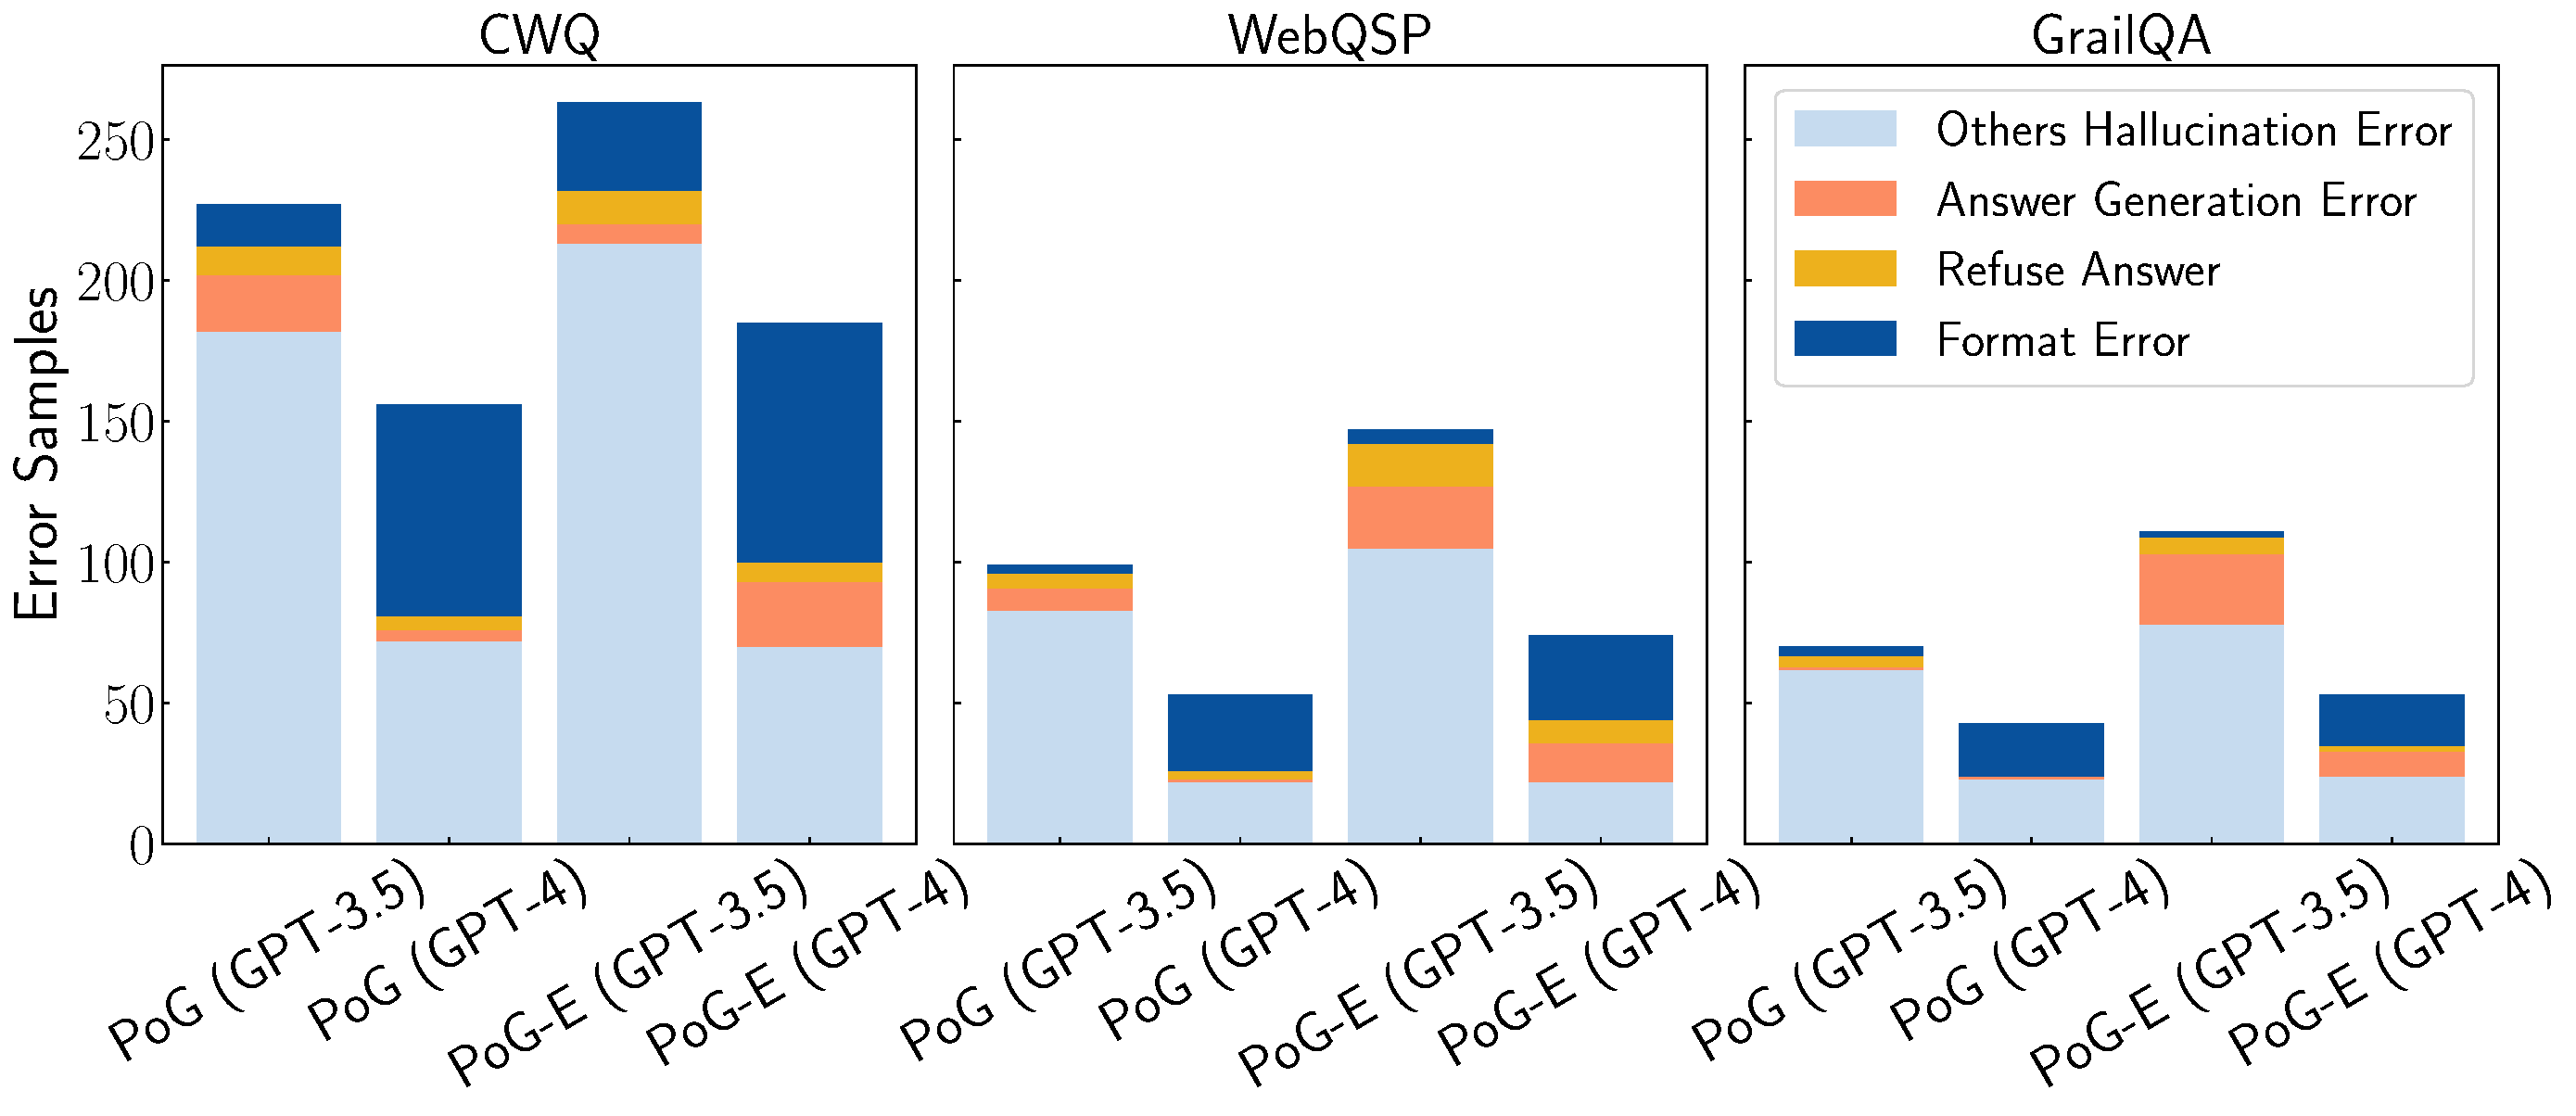
\includegraphics[width=1\linewidth]{graphs/error_analysis_cwq_three_datasets.pdf}
    \caption{The error instances and categories of PoG and PoG-E in the CWQ, WebQSP, and GrailQA datasets.}
    \label{fig:exp:error_analysis}
\end{figure}

% \newpage
\subsection{Efficiency Analysis}\label{appendix:exp:llm_calls}
\myparagraph{LLM calls cost analysis}
To evaluate the cost and efficiency of utilizing LLMs, we conducted an analysis of LLM calls on the CWQ, WebQSP, and GrailQA datasets. Initially, we examined the proportion of questions answered with varying numbers of LLM calls, as depicted in Figure \ref{fig:LLM_call_percentage}. The results indicate that the majority of questions are answered within nine LLM calls across all datasets, with approximately 80\% and 50\% of questions being resolved within six calls on CWQ and WebQSP, respectively. These findings demonstrate PoG's efficiency in minimizing LLM usage costs.
Furthermore, we compared the average number of LLM calls required by PoG with the current SOTA method, ToG \cite{tog1.0sun2023think}, as shown in Table \ref{fig:llmcall_vs_tog}. 
Since we utilized identical datasets for WebQSP, GrailQA, Simple Questions, and WebQuestions, we report the ToG results from their paper. The comparison reveals that PoG achieves comparable or superior accuracy while reducing the number of LLM calls by up to 40\% on the GrailQA dataset compared to ToG. This improvement is attributed to PoG's dynamic exploration strategy, which avoids starting from scratch, and its effective use of graph structures to prune irrelevant information, thereby significantly decreasing computational costs.

\begin{figure}[h]
    \centering
    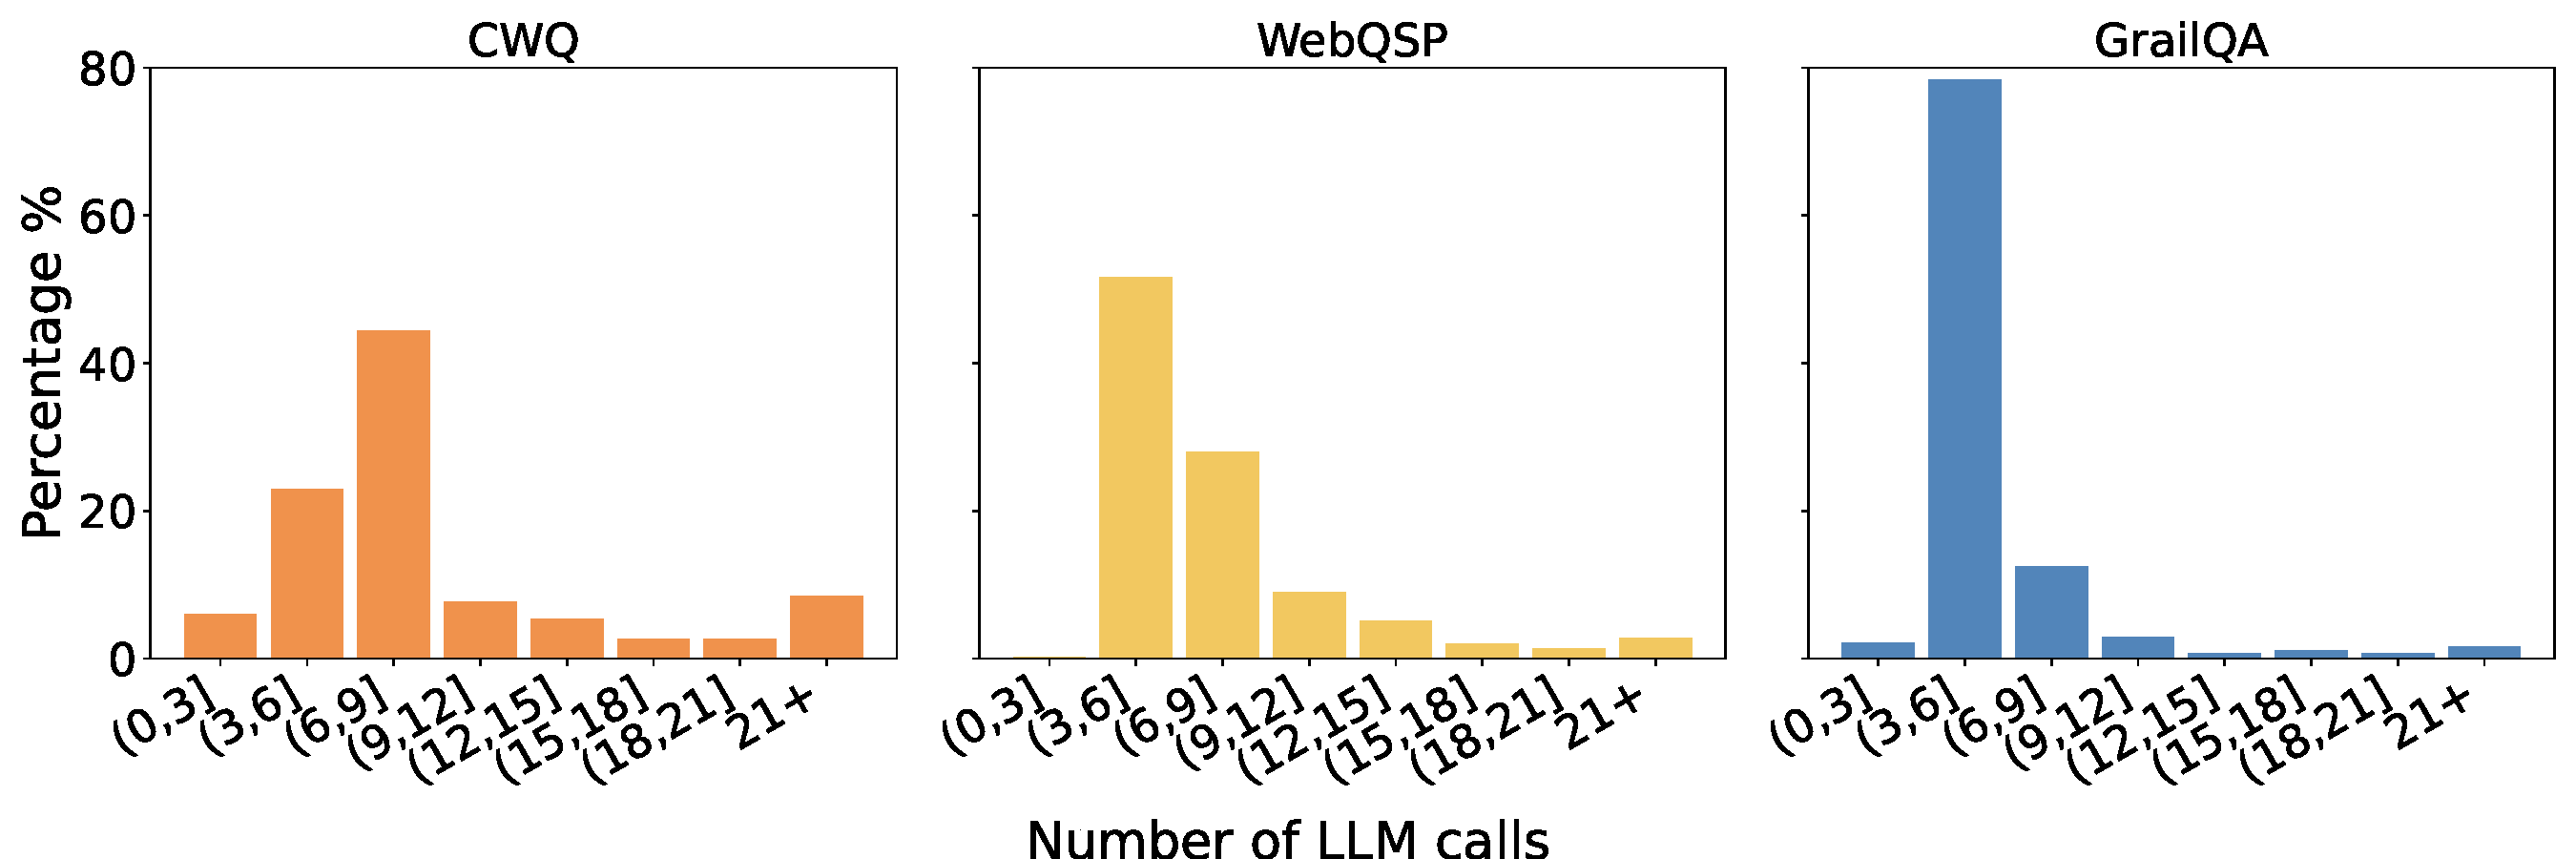
\includegraphics[width=1\linewidth]{graphs/LLM_Calls.pdf}
    
    \caption{The proportion of question of PoG and PoG-E by different LLM Calls among CWQ, WebQSP, and GrailQA datasets}
    \label{fig:LLM_call_percentage}
\end{figure}
% Please add the following required packages to your document preamble:
% \usepackage{booktabs}
% Please add the following required packages to your document preamble:
% \usepackage{booktabs}
\begin{table}[h]

\caption{Average LLM calls per question of PoG and ToG among all datasets.}\label{fig:llmcall_vs_tog}
\setlength\tabcolsep{1 pt}
\resizebox{0.95\columnwidth}{!}{
\begin{tabular}{@{}cccccc@{}}
\toprule
\textbf{Method} & \textbf{CWQ}           & \textbf{WebQSP}       & \textbf{GrailQA}   & \textbf{Simple Questions} & \textbf{WebQuestions}    \\ \midrule
\textbf{PoG}    & \textbf{10.7} & \textbf{8.3} & \textbf{6.5} & \textbf{6.1} & \textbf{9.3}\\
\textbf{ToG}    & -             & 11.2         & 10.6  & 8.7  & 10.5         \\ \bottomrule
\end{tabular}
}
\end{table}

% \myparagraph{Running time analysis}
% To better illustrate the efficiency performance of PoG, we have conducted extensive evaluations focusing on average accuracy, LLM call frequency, and running time on the multi-hop question datasets GrailQA and CWQ. The Table \ref{fig:running_cost_analysis} presents the performance of ToG and PoG with different beam search strategies.
% The result indicates, while improving accuracy may slightly increase runtime, our experiments show that PoG maintains an acceptable balance. PoG can reduce LLM call costs by up to 53.5\% while boosting accuracy by as much as 33.4\%. Within the PoG framework, users can select the most suitable variant based on their requirements for accuracy, cost, and runtime. All PoG setting provide significantly lower costs. For example, on the GrailQA dataset, using PoG-B allows users to achieve a 39.6\% reduction in LLM call costs and a 33.1\% improvement in accuracy with only a 1.14\% increase in runtime. A similar trend is also observed in the CWQ dataset.
\newpage
\myparagraph{Running time analysis}
To further evaluate the processing efficiency of PoG, we conducted extensive evaluations focusing on average accuracy, LLM call frequency, and running time on multi-hop question datasets GrailQA and CWQ. The results, presented in Table \ref{fig:running_cost_analysis}, compare the performance of ToG and PoG across various beam search strategies. The data indicate that while higher accuracy slightly increases runtime, PoG effectively balances accuracy with reduced LLM call costs. Specifically, PoG reduces LLM call costs by up to 53.5\% while increasing accuracy by up to 33.4\%. This allows users to tailor the PoG framework to their specific needs regarding accuracy, cost, and runtime. All PoG setting provide significantly lower costs. For instance, on the GrailQA dataset, PoG with 3-step beam search reduces LLM call costs by 39.6\% and improves accuracy by 33.1\%, with only a 1.14\% increase in runtime. A similar trend is also observed in the CWQ dataset.



\begin{table}[h]
\caption{Running time evaluation of ToG and PoG with different beam search methods on CWQ and GrailQA.}\label{fig:running_cost_analysis}
\begin{tabular}{@{}llcc@{}}
% \small
\toprule
\textbf{Model}              & \textbf{Evaluation} & \textbf{CWQ}  & \textbf{GrailQA} \\ 
\midrule
ToG    & Accuracy           & 53.1    & 59.3            \\
                          & Time (s)         & \textbf{78.7}       & \textbf{14.8}         \\
                          & LLM Calls       & 21.3           & 10.1               \\ 
\midrule
PoG              & Accuracy              & \textbf{81.4} & \textbf{92.7}   \\
 & Time (s)         &118.9           & 21.4         \\
                          & LLM Calls   & 9.1           & 6.5             \\
\midrule
PoG              & Accuracy           & 79.8          & 92.4     \\
w/ 3-Step Beam Search  & Time (s)         & 87.5       & 15.0         \\
                          & LLM Calls       & 8.8         & 6.1       \\ 
\midrule
PoG      & Accuracy           & 57.1          & 83.0           \\
w/ Fuzzy Selection                          & Time (s)         & 109.7             & 15.7         \\
                          & LLM Calls       & \textbf{6.8}           & \textbf{4.7}             \\  \bottomrule
\end{tabular}
\end{table}


% Please add the following required packages to your document preamble:
% \usepackage{booktabs}

\newpage
\subsection{Case Study}\label{appendix:exp_case_study}
\myparagraph{Case study: graph reduction and path pruning}
We conducted a case study using the example question presented in Figure \ref{fig:overall} to illustrate the effects of graph pruning and path pruning on the graph structure. Figure \ref{fig:exp:casestudy1}(a) shows the results of graph pruning, where vertices in blue are selected as part of the question subgraph, and vertices in black are pruned. In this sample, the number of entities is reduced from 16,740 to 1,245, resulting in a 92\% reduction of vertices.
Figures \ref{fig:exp:casestudy1}(b) and \ref{fig:exp:casestudy1}(c) demonstrate the question subgraph induced by the blue vertices in Figure \ref{fig:exp:casestudy1}(a) and the results after applying fuzzy and precise path selection. In these figures, vertices in blue represent the selected entity after each pruning, vertices in yellow represent the topic entities, and the vertex in red denotes the final answer entity.
From these graphs, we observe that utilizing the graph structure allows for the rapid pruning of irrelevant vertices, ensuring that the reasoning paths remain faithful and highly relevant to the question since all vertices within the question subgraph are interconnected with all topic entities, thereby maintaining the integrity and relevance of the reasoning process.
\begin{figure}[h]
    \begin{subfigure}{0.49\linewidth}
           \centering
           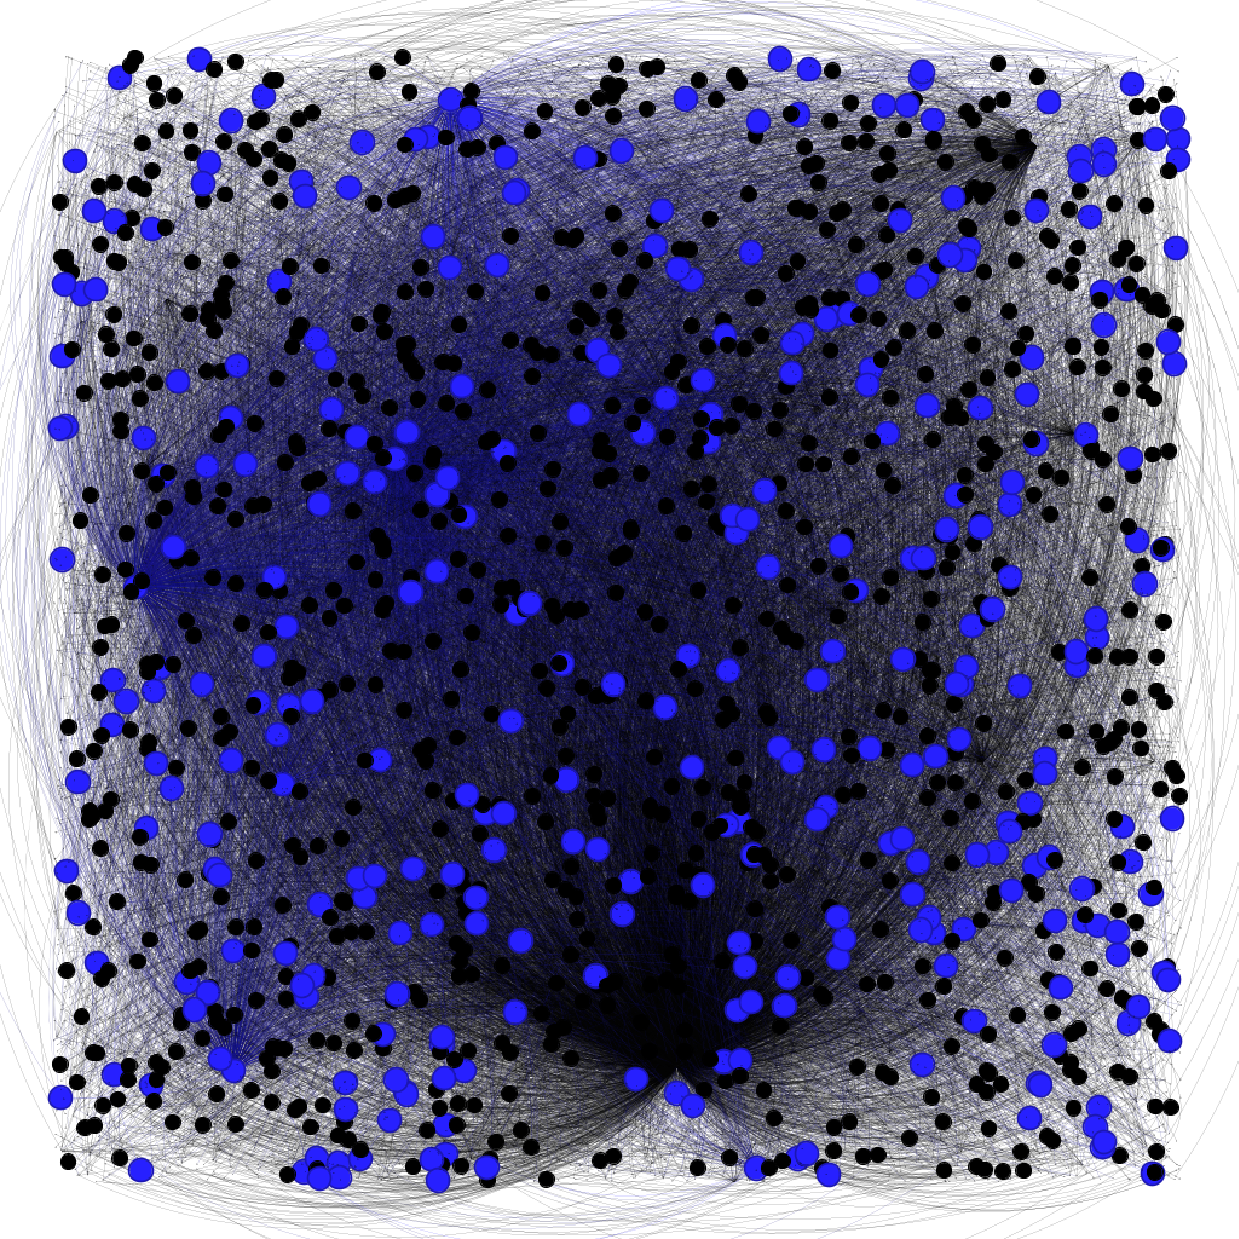
\includegraphics[width=1\linewidth]{graphs/QPathgraph2.pdf}
           
           \caption{Graph pruning}
    \end{subfigure}
    \begin{subfigure}{0.49\linewidth}
           \centering
           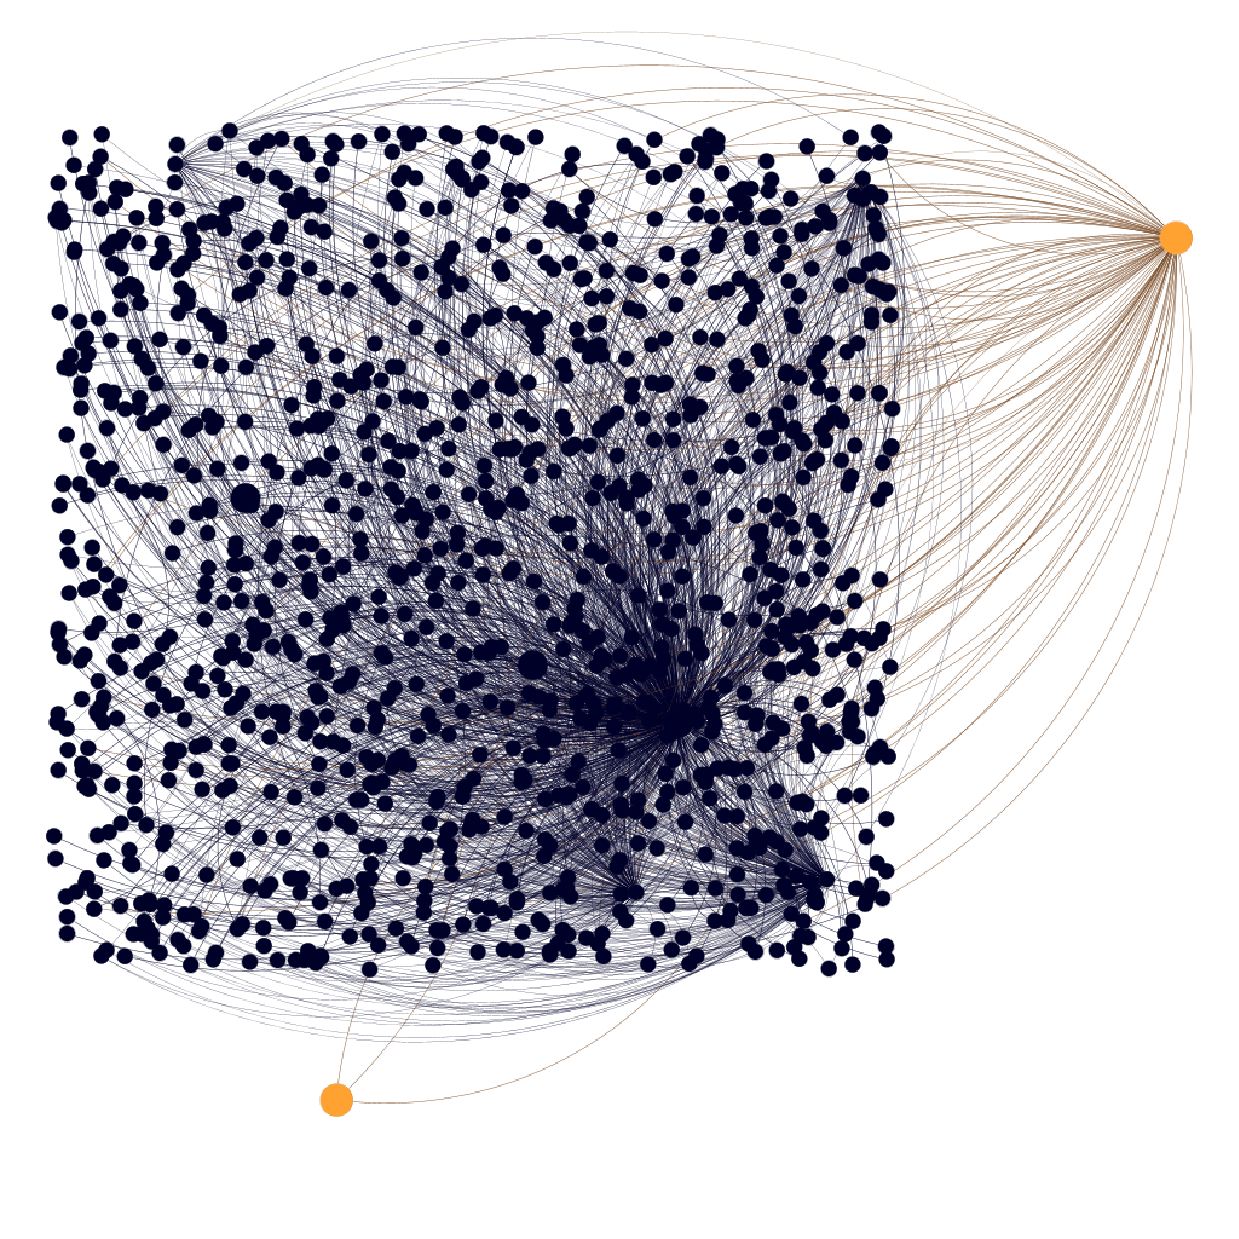
\includegraphics[width=1\linewidth]{graphs/path_graph.pdf}
           
           \caption{Question subgraph}
    \end{subfigure}
    \begin{subfigure}{0.49\linewidth}
           \centering
           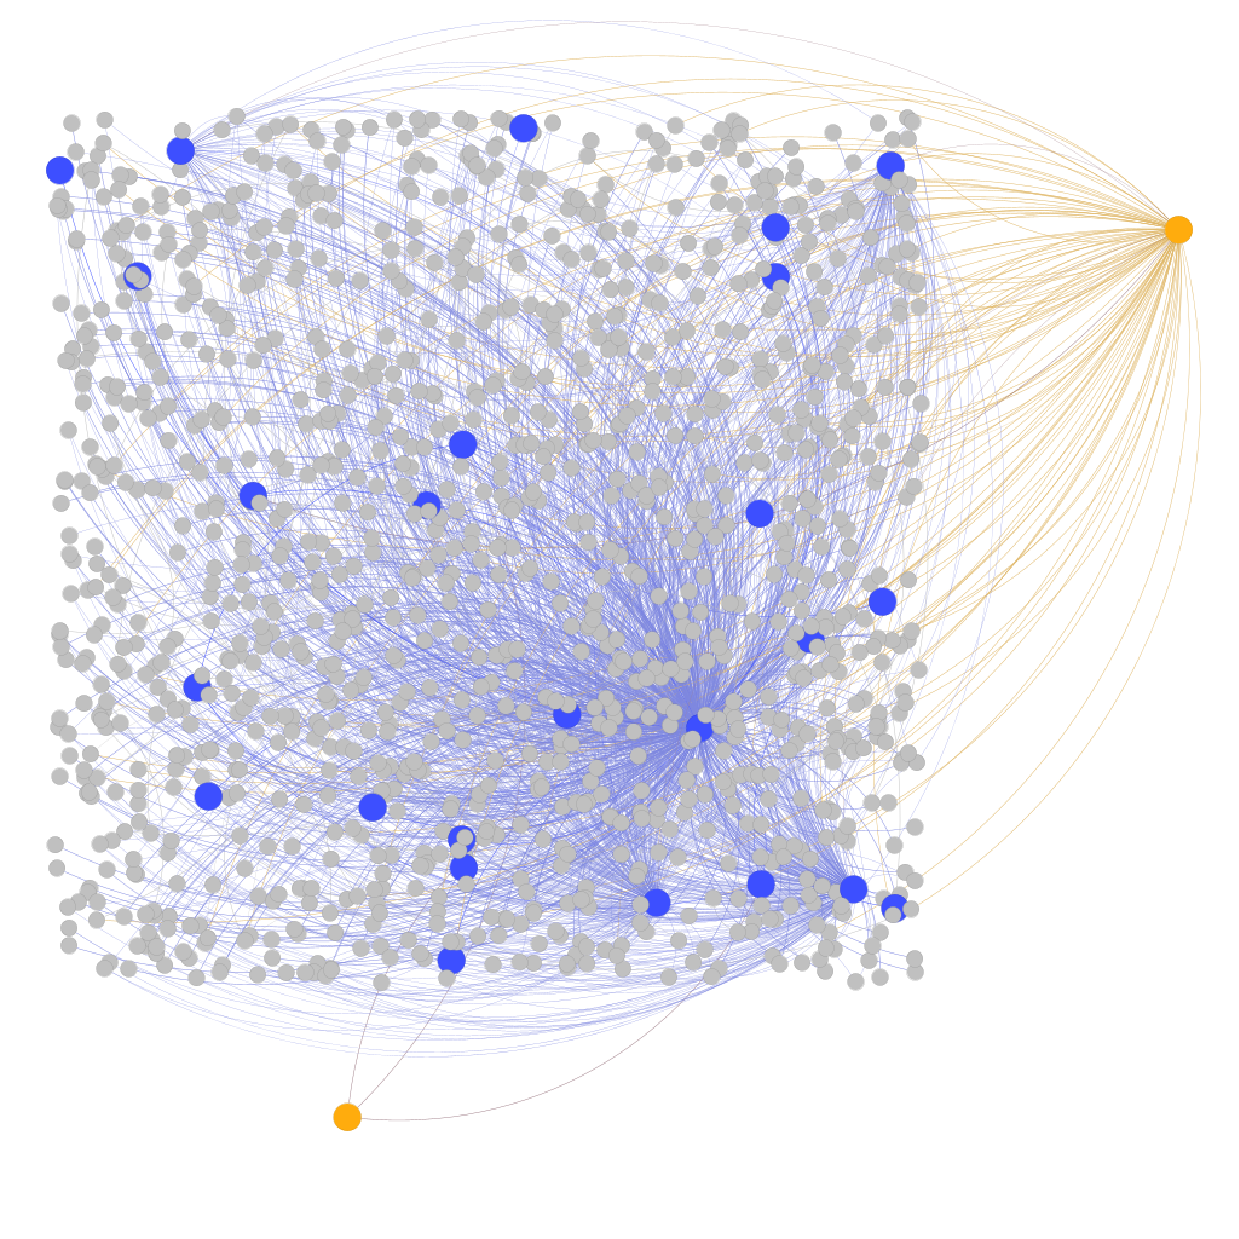
\includegraphics[width=1\linewidth]{graphs/beam_search_1.pdf}
           
           \caption{Fuzzy selection}
    \end{subfigure}
    \begin{subfigure}{0.49\linewidth}
           \centering
           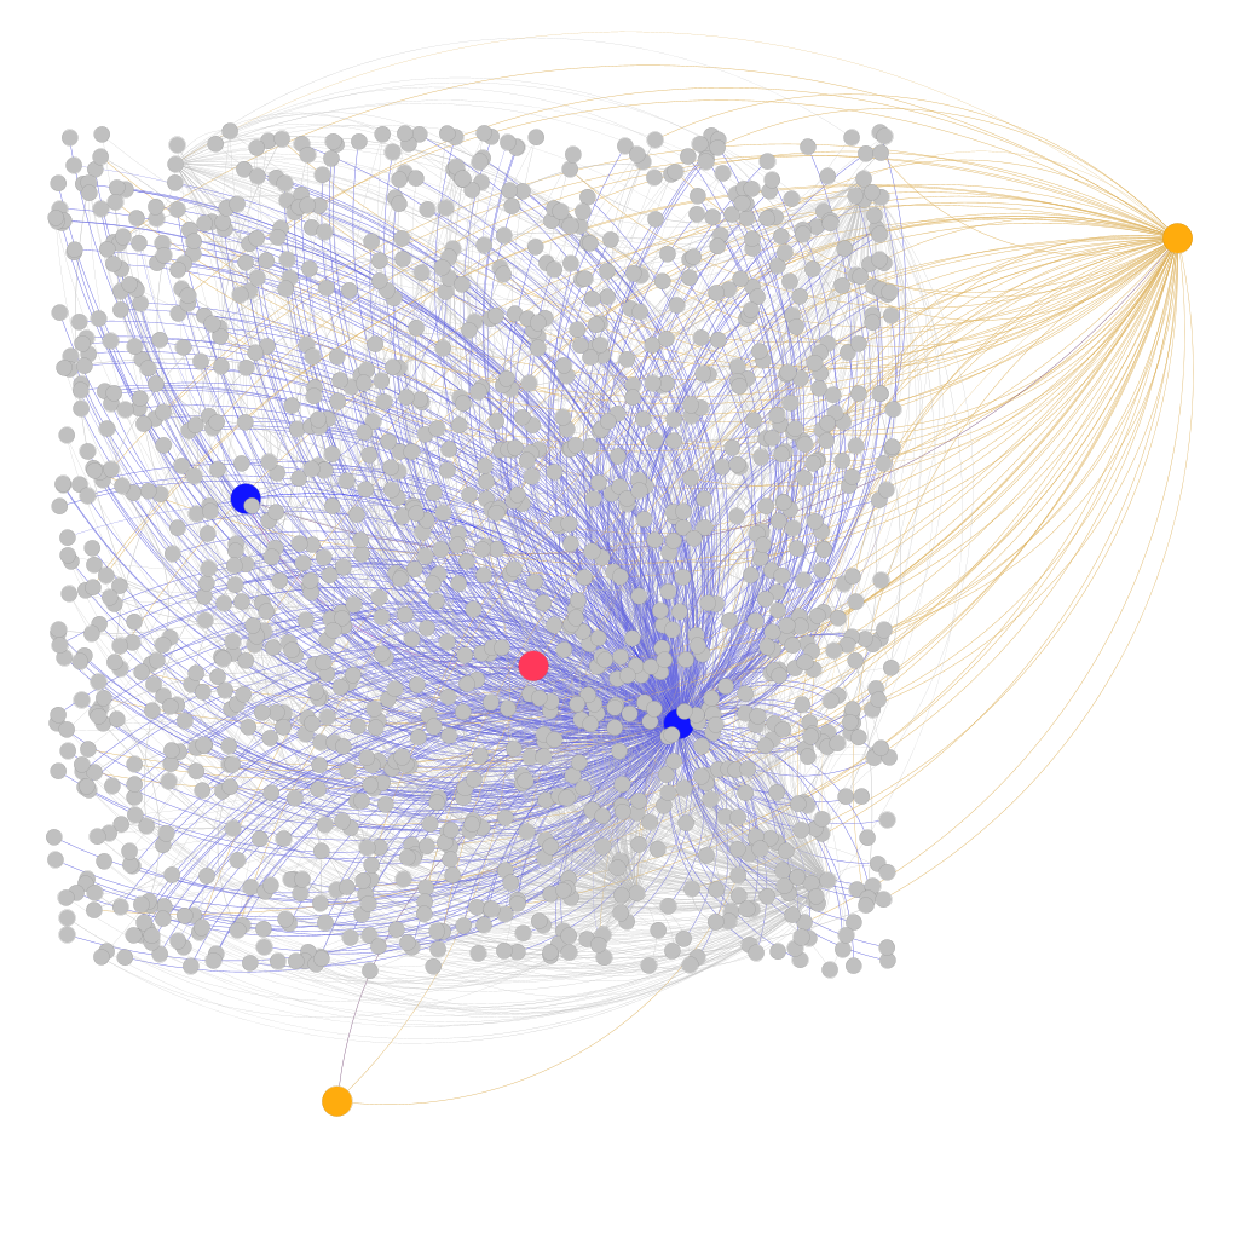
\includegraphics[width=1\linewidth]{graphs/answer.pdf}
           
           \caption{Precise selection}
    \end{subfigure}
    
\caption{Visualization of graph reduction and Path selection.}\label{fig:exp:casestudy1}
\end{figure}




\myparagraph{Case study: interpretable reasoning}
In this section, we present Table \ref{fig:exp:case:interpre}, which illustrates PoG's interpretability through case studies involving questions with one, two, and three entities. These examples demonstrate PoG's effectiveness in handling multi-entity and multi-hop tasks by providing clear and understandable reasoning paths that lead to accurate answers.

\begin{table*}[]
\centering
\vspace{4mm}
\caption{Examples of faithful and interpretable reasoning of PoG.} \label{fig:exp:case:interpre}
% 
\label{tab:case_int}
\begin{tabularx}{0.9\textwidth}{@{}p{3cm}X@{}} 
\toprule
\textbf{Field} & \textbf{Content} \\ 
\midrule
\textbf{Question} & Lou Seal is the mascot for the team that last won the World Series when? \\ 
\textbf{Answer} & 2014 World Series \\
\textbf{Topic Entity} & \textbf{Lou Seal} \\
\toprule
\textbf{LLM indicator} & "\textbf{Lou Seal}" - mascot for - team - last won - World Series - when \\
\textbf{Split Question} & split\_question 1: What team is "Lou Seal" the mascot for? \\

& split\_question 2: When did the last World Series win occur for the team with Lou Seal as the mascot?\\
\toprule
\textbf{Reasoning Path} & \{\textbf{Lou Seal}\} $\rightarrow$ sports.mascot.team $\rightarrow$ \{San Francisco Giants\} $\rightarrow$ sports.sports\_team.championships $\rightarrow$ \{\textcolor{red}{\textbf{2014 World Series}}, 2012 World Series, 2010 World Series\} \\
\toprule
\textbf{PoG answer} & 
\textbf{answer}: \{\textcolor{red}{\textbf{2014 World Series}}\} \\

 & \textbf{reason}: From the given path \{Lou Seal\} $\rightarrow$ sports.mascot.team $\rightarrow$ \{San Francisco Giants\}, \{San Francisco Giants\} is the team that "Lou Seal" serves as the mascot for. From \{San Francisco Giants\} $\rightarrow$ sports.sports\_team.championships $\rightarrow$ \{2014 World Series, 2012 World Series, 2010 World Series\}, the last World Series won by the \{San Francisco Giants\} is in \{2014\}. Therefore, the provided knowledge graph path is sufficient to answer the overall question, and the answer is \{2014 World Series\}.\\
\bottomrule


\midrule
\textbf{Question} & What European Union country sharing borders with Germany contains the Lejre Municipality? \\ 
\textbf{Answer} & Denmark \\
\textbf{Topic Entity} & \textbf{\{Germany, Lejre Municipality\}} \\
\toprule
\textbf{LLM indicator} & "\textbf{Lejre Municipality}" – contained by - European Union country (answer)- shares borders with-"\textbf{Germany}" \\
\textbf{Split Question} & split\_question 1: What European Union country shares borders with "Germany"? \\
& split\_question 2: What country contains the Lejre Municipality?\\
\toprule
\textbf{Reasoning Path} &\{\textbf{Lejre Municipality}\} $\rightarrow$ location.administrative\_division.country $\rightarrow$ \{\textcolor{red}{\textbf{Denmark}}\} $\rightarrow$ location.location.containedby $\rightarrow$ \{Eurasia\} $\rightarrow$ location.location.contains $\rightarrow$ \{\textbf{Germany}\}, \\
&\{\textbf{Lejre Municipality}\} $\rightarrow$ location.administrative\_division.country $\rightarrow$ \{\textcolor{red}{\textbf{Denmark}}\} $\rightarrow$ base.locations.countries. continent $\rightarrow$ \{Europe\} $\rightarrow$ location.location.contains $\rightarrow$ \{Western Europe\} $\rightarrow$ location.location.contains $\rightarrow$ \{\textbf{Germany}\}\\
\toprule
\textbf{PoG answer} & 
\textbf{answer}: \{\textcolor{red}{\textbf{Denmark}}\} \\

 & \textbf{reason}: From \{Denmark\} $\rightarrow $ location.location.containedby $\rightarrow$ \{Eurasia\} $\rightarrow$location.location.contains $\rightarrow$ \{Germany\}, Denmark is European Union country shares borders with "Germany". From \{Lejre Municipality\} $\rightarrow$ location.administrative\_division.country $\rightarrow$ \{Denmark\}, Denmark is a country contains the Lejre Municipality Both paths lead to Denmark, which is the European Union country sharing borders with Germany and containing the Lejre Municipality. Therefore, the provided knowledge graph path is sufficient to answer the main question, and the answer is \{Denmark\}.\\

\bottomrule


\midrule
\textbf{Question} & What Central Tiem Zone continent do the Falkland Islands belong to? \\ 
\textbf{Answer} & Americas \\
\textbf{Topic Entity} & \textbf{\{Falkland Islands, Continent, Central Time Zone\}} \\
\toprule
\textbf{LLM indicator} & answer("\textbf{Central Time Zone}") – owns - answer("\textbf{Continent}")- located contain -"\textbf{Falkland Islands}" \\
\textbf{Split Question} & split\_question 1:What continent do the Falkland Islands belong to? \\

& split\_question 2: What Central Time Zone does the continent belong to?\\
\toprule
\textbf{Reasoning Path} &\{\textbf{Central Time Zone}\} $\rightarrow$ time.time\_zone.locations\_in\_this\_time\_zone $\rightarrow$ \{\textcolor{red}{\textbf{Americas}}\} $\rightarrow$ common.topic.not able\_types  $\rightarrow$ \{\textbf{Continent}\} $\rightarrow$ common.topic. notable\_types  $\rightarrow$ \{Americas\} $\rightarrow$ location.location.con tains  $\rightarrow$\{ \textbf{Falkland Islands}\}\\
\toprule
\textbf{PoG answer} & 
\textbf{answer}: \{\textcolor{red}{\textbf{Americas}}\} \\

 & \textbf{reason}: From \{Continent\} $\rightarrow$ common.topic.notable\_types  $\rightarrow$ \{Americas\} $\rightarrow$ location.location. contains  $\rightarrow$\{ Falkland Islands\}, Americas  is the continent Falkland Islands belong to.
From \{Central Time Zone\} $\rightarrow$ time.time\_zone.locations\_in\_this\_time\_zone $\rightarrow$ \{Americas\} $\rightarrow$ common.topic. notable\_types  $\rightarrow$ \{Continent\}. Americas is the Central Time Zone.
Therefore, the provided knowledge graph path is sufficient to answer the overall question, and the answer is \{Americas\}.
\\

\bottomrule
\end{tabularx}
\end{table*}


\newpage
\section{Experiment Details}
\label{appen:dataset_details}
% Please add the following required packages to your document preamble:
% \usepackage{booktabs}
% The statistics of the datasets used in this paper are shown in Table \ref{table:datatsets}.
% We also provide a detailed result table for each dataset, shown in Table 10 to Table 18, illustrating the enhancements of ToG compared to the previous fine-tuning-based and prompting-based relevant works. For WebQSP, GrailQA, WebQuestion, ChatGPT-based PoG leads a new state-of-the-art.
% For CWQ, GPT4-based PoG leads a new state-of-the-art.
% Furthermore, GPT-4-based PoG exceeded the fine-tuning-based approaches on all Multi-Hop
% KBQA datasets, where on datasets CWQ, Simple Questions, PoG close to the state-of-the-art (83.9\%).


\myparagraph{Experiment datasets} To evaluate PoG's capability in multi-hop knowledge-intensive reasoning tasks, we assess it on four KBQA datasets: three multi-hop datasets (CWQ \cite{talmor-berant-2018-web}, WebQSP \cite{yih-etal-2016-value}, GrailQA \cite{grailqa}) and one single-hop dataset (SimpleQuestions \cite{simplequestions}). Additionally, to examine PoG on more general tasks, we include an open-domain QA dataset, WebQuestions.
For the evaluation of large datasets such as CWQ, GrailQA, and SimpleQuestions, we utilize a random sample of 1,000 test cases from CWQ and employ the 1,000 samples previously reported by ToG \cite{tog1.0sun2023think} to facilitate a comparison with the SOTA while also minimizing computational costs. Freebase serves as the background knowledge graph for all datasets, which encompasses approximately 88 million entities, 20,000 relations, and 126 million triples \cite{rogluo2023reasoning, freebase}. The statistics of the datasets utilized in this study are detailed in Table \ref{fig:appendix:dataset}. The source code has been publicly available\footnote{https://github.com/SteveTANTAN/PoG}.


\myparagraph{Baselines} 
Inspired by ToG \cite{tog1.0sun2023think}, we compare our method with standard prompting (IO), Chain-of-Thought (CoT), and Self-Consistency (SC) promptings with six in-context exemplars and "step-by-step" reasoning chains. For each dataset, we also include previous SOTA works for comparison. 
For a fair play, we compare with previous SOTA among all prompting-based methods and previous SOTA among all methods respectively.
Since ToG is the current SOTA prompting-based method, we directly refer to their results and those of other baselines reported in their paper for comparisons.


\myparagraph{Experimental implementation}
Leveraging the plug-and-play convenience of our framework, we experiment with two LLMs: GPT-3.5 and GPT-4. We use the OpenAI API to access GPT-3.5 (GPT-3.5-turbo) and GPT-4. Aligning with ToG, we set the temperature parameter to 0.4 during the exploration process (to increase diversity) and to 0 during the reasoning process (to ensure reproducibility). The maximum token length for generation is set to 256.
In all experiments, we set both $W_{\max}$ and $D_{\max}$ to 3 for beam search. All the experiments are conducted on a machine with Intel Xeon
Gold 6248R CPU, Nvidia A5000 GPU and 512GB memory.


% In addition, comprehensive results are presented for each data set,
% highlighting the advancements achieved by ToG over prior fine-tuning-based and prompting-based methods. Notably, for the datasets WebQSP, GrailQA, and WebQuestions, PoG based on ChatGPT establishes a new state-of-the-art. Similarly, for CWQ, PoG powered by GPT-4 sets a new benchmark.
% Moreover, GPT-4-based PoG surpasses fine-tuning-based methods across all Multi-Hop KBQA datasets. Specifically, in datasets such as CWQ and Simple Questions, PoG's performance approaches the state-of-the-art, achieving an accuracy of 83.9\%.



\begin{table}[H]
% \caption{The statistics of the datasets used in this paper. $^\dagger$ denotes we randomly selected 1,000 samples from the CWQ test set to constitute the testing set owing to the abundance of test samples.
% $^\ast$ denotes wee utilize the 1,000 samples reported by ToG\cite{tog1.0sun2023think} to compare with the state-of-the-art.}\label{fig:appendix:dataset}
% \vspace{mm}
\caption{
Statistics of the datasets used in this paper. 
$^\dagger$ denotes we randomly select 1,000 samples from the CWQ test set to create the experiment testing set due to the abundance of test samples.
$^\ast$ denotes that we utilize the 1,000 samples reported by ToG \cite{tog1.0sun2023think} to compare with the state-of-the-art.
}\label{fig:appendix:dataset}

\setlength\tabcolsep{1 pt}
\resizebox{0.95\columnwidth}{!}{
% Please add the following required packages to your document preamble:
% \usepackage{booktabs}
\begin{tabular}{@{}cccc@{}}
\toprule
Dataset             & Answer Format & Test  & Train \\ \midrule
ComplexWebQuestions (CWQ) $^\dagger$ & Entity        & 1,000 & 27,734                    \\
WebQSP              & Entity/Number & 1,639 &  3,098                      \\
GrailQA$^\ast $           & Entity/Number & 1,000 & 44,337                      \\
Simple Question$^\ast$    & Entity/Number & 1,000 &  14,894                       \\
WebQuestions        & Entity/Number & 2,032 & 3,778                      \\ \bottomrule
\end{tabular}
}
\end{table}

\newpage
\section{SPARQL}\label{appendix:aparql}
This section outlines the pre-defined SPARQL queries used for interacting with the knowledge graph and constructing graphs for our experiments. 

% \subsubsection{Pre-defined Sparql}
\subsection{1-hop Entity and Relation Search}\label{appendix:1_hop_e_r_search}
To facilitate the retrieval of 1-hop neighbors of entities within the Freebase Knowledge Graph, we have predefined a SPARQL query. This query is designed to be executed by simply substituting the appropriate ID for the query entity ID. It returns the connected entities' IDs and their associated relations' IDs, indicating whether the connected entity is at the tail or the head of the relation.

\lstset{language=SPARQL}
\begin{lstlisting}
PREFIX ns: <http://rdf.freebase.com/ns/>
SELECT ?|\textcolor{cyan}{relation}| ?|\textcolor{red}{connectedEntity}| ?direction
WHERE {
    {
        ns:|\textcolor{purple}{ID}| ?|\textcolor{cyan}{relation}| ?|\textcolor{red}{connectedEntity}| .
        BIND(|\textcolor{olive}{"tail"}| AS ?direction)
    }
    UNION
    {
        ?|\textcolor{red}{connectedEntity}| ?|\textcolor{cyan}{relation}| ns:|\textcolor{purple}{ID}| .
        BIND(|\textcolor{orange}{"head"}| AS ?direction)
    }
}
\end{lstlisting}

% \newpage
\subsection{Short Textual Description}\label{appendix:short_D}
The following predefined function implements the retrieval of short textual descriptions, $\mathcal{D}(.)$, for converting the identifiers (IDs) of entities or relations into natural language descriptions.



\lstset{language=SPARQL}
\begin{lstlisting}
PREFIX ns: <http://rdf.freebase.com/ns/>
SELECT DISTINCT ?|\textcolor{cyan}{tailEntity}|
WHERE {
    {    
        ?|\textcolor{brown}{entity}| ns:type.object.name ?|\textcolor{cyan}{tailEntity}| .
        FILTER(?|\textcolor{brown}{entity}| = ns:|\textcolor{purple}{ID}|)  
    }  
    UNION
    {    
        ?|\textcolor{brown}{entity}| <http://www.w3.org/2002/07/owlsameAs> ?|\textcolor{cyan}{tailEntity}| .    
        FILTER(?|\textcolor{brown}{entity}| = ns:|\textcolor{purple}{ID}|)  
    }
}

\end{lstlisting}

% \subsubsection{1-hop Subgraph Search}
% To realize the subgraph detection in section \ref{method:1.1subgraphD}, we implement the 1-hop subgraph detection, which is the combination of previous Sparql function in appendix \ref{appendix:1_hop_e_r_search} \& \ref{appendix:short_D}
% In this function, by given the query entity ID, we can obtain its 1-hop neighbors' ID, natural language name, and their associated relations, indicating whether the connected entity is at the tail or the head of the relation, in one Sparql query. 

\newpage
\subsection{1-hop Subgraph Search}
To facilitate subgraph detection in Section \ref{method:initialization}, we implement the 1-hop subgraph detection feature by integrating SPARQL functions described in Appendix \ref{appendix:1_hop_e_r_search} and \ref{appendix:short_D}. The purpose of this function is to retrieve, in a single SPARQL query, the 1-hop neighbors of a given query with their IDs, natural language names, and connected relationships, specifying whether the connected entity is at the tail or the head of the relationship.
\lstset{language=SPARQL}
\begin{lstlisting}
PREFIX ns: <http://rdf.freebase.com/ns/>
SELECT ?|\textcolor{cyan}{relation}| ?|\textcolor{red}{connectedEntity}| ?|\textcolor{teal}{connectedEntityName}| ?direction
WHERE {
    {
        ns:|\textcolor{purple}{ID}| ?|\textcolor{cyan}{relation}| ?|\textcolor{red}{connectedEntity}| .
        OPTIONAL {
            ?|\textcolor{red}{connectedEntity}| ns:type.object.name ?name .
            FILTER(lang(?name) = 'en')
        }
        BIND(COALESCE(?name, |\textcolor{black}{"Unnamed Entity"}|) AS ?|\textcolor{teal}{connectedEntityName}|)
        BIND(|\textcolor{olive}{"tail"}| AS ?direction)
    }
    UNION
    {
        ?|\textcolor{red}{connectedEntity}| ?|\textcolor{cyan}{relation}| ns:|\textcolor{purple}{ID}| .
        OPTIONAL {
            ?|\textcolor{red}{connectedEntity}| ns:type.object.name ?name .
            FILTER(lang(?name) = 'en')
        }
        BIND(COALESCE(?name, |\textcolor{black}{"Unnamed Entity"}|) AS ?|\textcolor{teal}{connectedEntityName}|)
        BIND(|\textcolor{orange}{"head"}| AS ?direction)
    }
}
\end{lstlisting}

\newpage
\onecolumn
\section{Prompts}\label{appendix:prompt}
In this section, we detail the prompts required for our main experimental procedures.

\begin{center}
\begin{minipage}{0.7\columnwidth}
    \vspace{2mm}
        \centering
    \begin{tcolorbox}[title=Question Analysis Prompt Template] 
        \small
            % \centering
    You will receive a multi-hop question, which is composed of several interconnected queries, along with a list of topic entities that serve as the main keywords for the question. Your task is to break the question into simpler parts, using each topic entity once and provide a Chain of Thought (CoT) that shows how the topic entities are related. Note: Each simpler question should explore how one topic entity connects to others or the answer. The goal is to systematically address each entity to derive the final answer.
\vspace{5pt}
    
    \texttt{In-Context Few-shot}
\vspace{5pt}
    
    Q: \{Query\} 
    
    Topic Entity: \{Topic Entity\} 
    
    A: 
    \end{tcolorbox}
    % \vspace{1mm}
    \vspace{2mm}

\end{minipage}
\end{center}

\begin{center}
\begin{minipage}{0.7\columnwidth}
    % \centering
    \vspace{2mm}
    \begin{tcolorbox}[title=LLM Supplement Prompt Template]~\label{prompts_LLM_Supplement}
        \small
Using the main question, a possibly uncertain chain of thought generated by a language model, some related split questions, paths from the "Related\_paths" section, and main topic entities:
please first provide three predicted results,
and second offer three possible chains of thought that could lead to these results, using the provided knowledge paths and your own knowledge.
If any answers are unclear, suggest alternative answers to fill in the gaps in the chains of thought, following the same format as the provided examples.

\vspace{5pt}

\texttt{In-Context Few-shot}
\vspace{5pt}

Q: \{Query\} 

Topic Entity: \{Topic Entity\} 

Think Indicator:\{Think Indicator\}

Split Question:\{Split Question\}

A: 
    \end{tcolorbox}
    \vspace{2mm}
\end{minipage}
\end{center}
where \texttt{\{Think Indicator\}, \text{and} \{Split Question\}} are obtained in section \ref{method:initialization}. An indicator example is shown in Figure \ref{fig:overall}.

\begin{center}
    
\begin{minipage}{0.7\columnwidth}
    \centering
    % \vspace{pt}
    \vspace{2mm}
    
    \begin{tcolorbox}[title=Precise Path Select Prompt Template]
        \small
Given a main question, a LLM-generated thinking Cot that considers all the entities, a few split questions that you can use one by one and finally obtain the final answer, and the associated retrieved knowledge graph path, \{set of entities (with id start with "m.")\} -> \{set of relationships\} -> \{set of entities(with id start with "m.")\}, 
Please score and give me the top three lists from the candidate paths set can be highly to be the answer of the question.

\vspace{5pt}
    
\texttt{In-Context Few-shot}

\vspace{5pt}
Q: \{Query\} 

Think Indicator:\{Think Indicator\}

Split Question:\{Split Question\}

Candidate Paths:\{Candidate Paths\}

A: 
\end{tcolorbox}
\vspace{2mm}
\end{minipage}
\end{center}
\texttt{\{Candidate Paths\}} denotes the retrieved reasoning paths $Final_paths$ to be selected in this request which are formatted as a series of structural sentences:

\begin{minipage}{0.99\columnwidth}
    \centering
    $\{e_{0x},...,e_{0z}\}\to r_{1_i} \to \{e_{1x},...,e_{1z}\}\to \dots$ $\to r_{l_j} \to \{e_{lx},...,e_{lz}\}$ 
    \\ $\dots$\\
    $\{e_{0x},...,e_{0z}\}\to r_{1_i} \to \{e_{1x},...,e_{1z}\}\to \dots$ $\to r_{l_j} \to \{e_{lx},...,e_{lz}\}$,
    % \vspace{5pt}
    
\end{minipage}

\noindent where, $i$ and $j$ in $r_{1_i}, r_{1_i}$ represent the $i$-th, $j$-th relation from each relation edge in the clustered question subgraph.
And $e$ is constructed by its ID and natural language name $\mathcal{D}(ID)$.
\vspace{5pt}

\begin{center}
    
\begin{minipage}{0.7\columnwidth}
    % \centering
    \vspace{2mm}
    \begin{tcolorbox}[title=Path Summarizing Prompt Template]
        \small
Given a main question, an uncertain LLM-generated thinking Cot that considers all the entities, a few split questions that you can use one by one and finally obtain the final answer, the associated accuracy retrieved knowledge paths from the Related paths section, and main topic entities.
Your task is to summarize the provided knowledge triple in the Related paths section and generate a chain of thoughts by the knowledge triple related to the main topic entities of the question, which will used for generating the answer for the main question and split question further.
You have to make sure you summarize correctly by using the provided knowledge triple, you can only use the entity with id from the given path and you can not skip in steps.


\vspace{5pt}
    
\texttt{In-Context Few-shot}

\vspace{5pt}
Q: \{Query\} 

Think Indicator:\{Think Indicator\}

Split Question:\{Split Question\}

Related Paths:\{Related Paths\}

A: 
    \end{tcolorbox}
    \vspace{2mm}
\end{minipage}
\end{center}

    % \vspace{5pt}

\noindent\texttt{\{Related\_Paths\}} has the same format with the \texttt{\{Candidate\_Paths\}} before.
    % \vspace{5pt}

\begin{center}
    
\begin{minipage}{0.7\columnwidth}
    % \centering
    \vspace{2mm}
    
    \begin{tcolorbox}[title= Question Answering Evaluation Prompt Template]
        \small
Given a main question, an uncertain LLM-generated thinking Cot that considers all the entities, a few split questions that you can use and finally obtain the final answer, and the associated retrieved knowledge graph path, \{set of entities (with id start with "m.")\} -> \{set of relationships\} -> \{set of entities(with id start with "m.")\}.
Your task is to determine if this knowledge graph path is sufficient to answer the given split question first then the main question. 
If it's sufficient, you need to respond \{Yes\} and provide the answer to the main question. If the answer is obtained from the given knowledge path, it should be the entity name from the path. Otherwise, you need to response \{No\}, then explain the reason. 


\vspace{5pt}
    
\texttt{In-Context Few-shot}

\vspace{5pt}
Q: \{Query\} 

Think Indicator:\{Think Indicator\}

Split Question:\{Split Question\}

Related Paths:\{Related Paths\}

A: 
    \end{tcolorbox}
    \vspace{2mm}
\end{minipage}
\end{center}

\begin{center}

\begin{minipage}{0.7\columnwidth}
    % \centering
    \vspace{2mm}
    \begin{tcolorbox}[title= Question Answering Generation Prompt Template]
        \small
Given a main question, an uncertain LLM-generated thinking Cot that considers all the entities, a few split questions that you can use one by one and finally obtain the final answer, and the associated retrieved knowledge graph path, \{set of entities (with id start with "m.")\} -> \{set of relationships\} -> \{set of entities(with id start with "m.")\}, 
Your task is to generate the answer based on the given knowledge graph path and your own knowledge.

\vspace{5pt}
    
\texttt{In-Context Few-shot}

\vspace{5pt}
Q: \{Query\} 

Think Indicator:\{Think Indicator\}

Split Question:\{Split Question\}

Related Paths:\{Related Paths\}

A: 
    \end{tcolorbox}
    \vspace{2mm}
\end{minipage}
\end{center}




\end{document}
